\documentclass[a4paper,11pt]{report}
\usepackage[T1]{fontenc}
\usepackage[utf8]{inputenc}
\usepackage[italian]{babel}
\usepackage{geometry}
	\geometry{a4paper,top=2cm,bottom=2cm,left=2.5cm,right=2.5cm,heightrounded}
\usepackage{amsmath, amsthm, amssymb, mathtools}
\usepackage{siunitx}
\usepackage{resizegather}
	\addtolength{\jot}{4pt}
\usepackage{pgfplots, pgfplotstable, booktabs, array}
	\pgfplotsset{compat=1.16}
	\pgfplotstableset{
		col sep = comma,
		every head row/.append style={before row=\toprule, after row=\midrule},
		every last row/.append style={after row=\bottomrule},
		every column/.append style={sci, sci zerofill, sci e, sci precision = 2},
		string replace={NaN}{},
		empty cells with={-}
	}
\usepackage{listingsutf8}
	\lstset{inputencoding=utf8/latin1}
	\lstset{numbers=left, frame=tb, rulecolor=\color{black}}
	\lstset{framexleftmargin=3em, xleftmargin=3em}
	\lstset{tabsize=4}
	\lstset{captionpos=b, abovecaptionskip=1ex}
	\renewcommand{\lstlistingname}{Programma}
\usepackage{matlab-prettifier}
	\lstset{style=Matlab-editor}
\usepackage[scaled]{beramono}
	\lstset{basicstyle=\mlttfamily \small}
	\lstset{numberstyle=\mlttfamily \small \color{gray}}
\usepackage{caption, subcaption}
	\captionsetup{tableposition=top,figureposition=bottom}
	\captionsetup{justification=centering,font=small,labelfont=bf}
\usepackage{hyperref}
	\hypersetup{hidelinks}
\usepackage{afterpage}
\usepackage{microtype}

\newcommand{\N}{\mathbb{N}}
\newcommand{\Z}{\mathbb{Z}}
\newcommand{\Q}{\mathbb{Q}}
\newcommand{\R}{\mathbb{R}}
\newcommand{\C}{\mathbb{C}}
\newcommand{\lambdamax}{\lambda_{\text{max}}}
\newcommand{\lambdamin}{\lambda_{\text{min}}}
\newcommand{\abs}[1]{\left\lvert#1\right\rvert}
\newcommand{\norm}[1]{\left\lVert#1\right\rVert}
\newcommand{\code}[1]{\begin{small}\texttt{#1}\end{small}}
\newcommand{\deq}{\vcentcolon=}
\newcommand{\eqd}{=\vcentcolon}
\newcommand{\dx}{\, dx}
\newcommand{\dy}{\, dy}
\newcommand{\dt}{\, dt}
\newcommand{\ds}{\, ds}
\newcommand{\dc}{\, dc}
\newcommand{\grad}{\nabla}
\renewcommand{\Re}{\operatorname{Re}}
\renewcommand{\Im}{\operatorname{Im}}
\DeclareMathOperator{\Ker}{Ker}
\DeclareMathOperator{\Rank}{Rank}
\DeclareMathOperator{\spn}{span} % \span è già utilizzato da latex
\DeclareMathOperator{\tr}{tr}

\theoremstyle{definition}
\newtheorem*{defi}{Definizione}
\newtheorem{esem}{Esempio}[chapter]
\newtheorem*{prob}{Problema}

\theoremstyle{plain}
\newtheorem{teor}{Teorema}[chapter]
\newtheorem{lemm}[teor]{Lemma}
\newtheorem{prop}[teor]{Proposizione}
\newtheorem{coro}[teor]{Corollario}
\newtheorem{dimo}{Dimostrazione}

\theoremstyle{remark}
\newtheorem*{osse}{Osservazione}

\title{\Huge{\bf{
	Elaborato per il corso \\
	\emph{Modelli Numerici per la Simulazione}
}}}
\author{\huge{Bruno Degli Esposti}}
\date{\Large{Primavera 2021}}

\begin{document}

\maketitle

\tableofcontents
\pagestyle{headings}

\graphicspath{{./figures/capitolo1/}}
\lstset{inputpath = ./programs/capitolo1}
\pgfplotstableset{search path = ./tables/capitolo1}

\chapter{Introduzione}

Questo elaborato ha lo scopo di ripercorrere
gli argomenti più importanti del corso
\emph{Modelli numerici per la simulazione}, che ho frequentato
nell'anno accademico 2018/2019.
Secondo quanto visto a lezione, ho prestato 
particolare attenzione ai seguenti aspetti:
la formulazione e l'analisi di sistemi dinamici semplici ma significativi,
spesso tratti da modelli scientifici,
la loro discretizzazione tramite opportuni metodi numerici,
l'implementazione effettiva di questi metodi in ambiente MATLAB
e infine l'analisi critica dei dati numerici ottenuti dalle simulazioni
alla luce dei risultati teorici noti.
Come premessa a tutto ciò, mi è sembrato opportuno iniziare
l'elaborato con una riflessione sul concetto di errore nell'ambito
del calcolo scientifico.
%Questo elaborato ripercorre gli argomenti più importanti
%del corso \emph{Modelli numerici per la simulazione}, con particolare
%attenzione all'analisi di alcuni sistemi dinamici significativi,
%spesso tratti da modelli scientifici,
%a cui seguono una discretizzazione tramite opportuni metodi numerici,
%un'implementazione effettiva di questi metodi in ambiente MATLAB
%e un'analisi critica dei dati numerici ottenuti dalle simulazioni
%alla luce della teoria.
%Come premessa a tutto ciò, mi è sembrato opportuno iniziare
%l'elaborato con una riflessione sul concetto di errore nell'ambito
%del calcolo scientifico.

Prima, però, qualche precisazione di carattere tecnico.
Nonostante io abbia lavorato individualmente a questo elaborato,
ho preferito adottare la prima persona plurale in tutto il testo
per una questione di abitudine.
Sempre per la stessa ragione, ho preferito scrivere in inglese
i nomi delle funzioni e delle variabili nel codice MATLAB,
lasciando però i commenti in italiano.
La suddivisione dei capitoli segue fedelmente quella
del libro di testo di riferimento per il corso.

Il tipo di dato \code{table} ricorre spesso nel codice MATLAB,
perché l'ho usato per generare le tabelle e i grafici in modo automatico
all'interno del sorgente LaTeX (funzione offerta dal pacchetto \code{pgfplots}).
La colorazione automatica della sintassi è dovuta al
pacchetto \code{matlab-prettifier}, che estende il pacchetto \code{listings}.
Il codice che ho scritto è stato testato solo sulla release 2020b
di MATLAB, ma credo di non aver utilizzato alcuna funzionalità
particolarmente recente.

\section{Analisi dell'errore} \label{sec:errore}

L'affidabilità delle previsioni fornite dal calcolo scientifico
dipende in modo cruciale dalla capacità di comprendere,
stimare e mantenere sotto controllo gli errori durante l'intero processo di calcolo.
Senza pretese di completezza o generalità,
in questo capitolo andremo a elencare le principali fonti di errore.
Nessuna fonte è a priori trascurabile, perché
ciascuna di esse, nelle giuste circostanze, può risultare decisiva
nel proprio contributo all'errore complessivo.

A monte, è inevitabile che venga commesso un \emph{errore di modellizzazione}:
ogni teoria scientifica fa uso di modelli matematici, ma
un buon modello non è tanto un modello \emph{perfetto}%
\footnote{Infatti un tale modello, ammesso che esista,
non sarebbe meno complesso della realtà stessa.},
quanto un modello che, nella sua semplicità, è in grado di fornire descrizioni o
previsioni \emph{utili}, cioè affette da errori sufficientemente piccoli
per il contesto in cui il modello trova applicazione.
In altre parole, un buon modello è in grado di catturare
gli aspetti strettamente essenziali di un fenomeno
(in termini di grandezze, dinamiche, ecc),
andando invece a escludere tutto il resto.
%in modo consapevole quelli superflui

Una seconda fonte di errore è poi l'incertezza
a cui sono soggetti tutti i dati in ingresso al modello;
si parla in questo caso di \emph{errore sui dati}.
Non è possibile, infatti, misurare alcuna grandezza
naturale o sociale con precisione assoluta:
ogni quantità, sia essa determinata tramite inferenza statistica,
misurata sperimentalmente o fornita a sua volta da altri modelli,
è inevitabilmente soggetta a errore, e andrebbe pertanto rappresentata mediante una
distribuzione di probabilità, piuttosto che un singolo valore puntuale.
Questo approccio, ammesso che si sappia dire qualcosa su tali distribuzioni,
complica però di parecchio il modello; spesso ci si accontenta di tenere
traccia di intervalli di confidenza.
%(anche in senso generalizzato: ad esempio,
%l'incertezza di $\pm 0,05$mm associata alla misura con un calibro ventesimale, oppure
%la tolleranza del~5\% dichiarata da un costruttore di resistenze elettriche).
%Solitamente non spetta all'analista numerico occuparsi di questi tipi di errore.

Una terza fonte d'errore deriva dalle difficoltà computazionali
che si riscontrano durante l'applicazione del modello.
Quasi sempre, infatti, la soluzione del problema matematico
previsto dal modello non può essere calcolata in modo esatto
da un algoritmo che opera tramite un numero finito di operazioni elementari
sui dati iniziali; pertanto bisogna accontentarsi di
%un algoritmo che ne calcoli
un'approssimazione.%
\footnote{È un esempio celebre la soluzione per radicali
delle equazioni algebriche di grado 5 o superiore.}
In questo caso si parla di \emph{errore associato
al metodo numerico}. Questo è il tipo di errore che si manifesta,
ad esempio, ogni volta che un procedimento iterativo viene
arrestato prima di essere arrivato a convergenza, oppure
ogni volta che una serie numerica viene troncata, o magari quando
un integrale viene approssimato tramite una formula di quadratura.
Più nello specifico, in questo elaborato ci ritroveremo spesso ad analizzare
l'errore che si commette quando un ente matematico la cui natura è continua
%dalla natura continua
(un sistema dinamico, un oggetto geometrico, un operatore) viene sostituito
da un analogo ente discreto, sempre per esigenze computazionali: questo errore
è detto \emph{errore di discretizzazione}.

Un'ulteriore fonte di errore consiste nell'utilizzo di operazioni
aritmetiche inesatte all'interno di un algoritmo, al fine di velocizzarne
l'esecuzione e ridurne l'occupazione di memoria.
L'aritmetica esatta, laddove il suo uso sia possibile,
è infatti troppo onerosa da un punto di vista computazionale,
e per questo motivo viene utilizzata molto raramente nell'ambito del calcolo scientifico.
%(un uso possibile è la stima a posteriori dell'errore associato
%al metodo numerico).
Inoltre, sarebbe superfluo eseguire in modo esatto delle operazioni
aritmetiche su quantità comunque affette da errore,
secondo quanto detto nei punti precedenti. % (vedi punti precedenti).
Ad ogni modo, l'utilizzo dell'aritmetica inesatta non è privo di insidie:
bisogna assicurarsi che l'algoritmo scelto
non porti a un accumulo incontrollato dei piccoli%
\footnote{Anzi, a volte non proprio piccoli, come vedremo in seguito
parlando degli errori di cancellazione numerica.}
errori commessi da ogni operazione, detti \emph{errori dovuti all'aritmetica finita},
con conseguenze potenzialmente catastrofiche sull'accuratezza del risultato finale.
Lo studio di questo aspetto di un algoritmo è detto \emph{analisi di stabilità}:
formalmente un algoritmo di dice \emph{instabile} se, eseguito in aritmetica
inesatta, genera un errore sui dati in uscita di alcuni%
\footnote{Quanti, nella pratica? Non c'è una risposta univoca,
ma già quattro non ci sembrano trascurabili.}
ordini di grandezza maggiore dell'errore sui dati in ingresso al modello,
altrimenti si dice \emph{stabile}.
Non sempre è possibile trovare un'alternativa stabile a un algoritmo instabile:
talvolta è la natura stessa del problema matematico da risolvere che comporta
un'amplificazione massiccia degli errori sui dati in ingresso.
In questi casi, anche in assenza di errori associati al metodo numerico
o dovuti all'aritmetica finita, non si riuscirebbe comunque 
a determinare con precisione il valore in uscita dal modello;
si parla allora di \emph{problemi mal condizionati}.
Il fattore di proporzionalità tra gli errori sui dati in ingresso e gli
errori sui dati in uscita è detto \emph{numero di condizionamento del problema}.
Dunque, il numero di condizionamento di un problema pone un limite intrinseco
alla stabilità di qualunque algoritmo impiegato per risolvere il modello.
Un esempio estremo di problema mal condizionato è la simulazione
di un sistema dinamico caotico, come vedremo più avanti nel Capitolo 7.
Tornando all'aritmetica inesatta,
%
%questo tipo di errore è, in un certo senso, quello fondamentale, perché
%fornisce una limitazione inferiore a tutti gli altri tipi di errore.
%Inoltre stabilisce implicitamente se gli altri errori vadano calcolati
%in senso assoluto (nel caso dei numeri a virgola fissa) o relativo (nel caso
%dei numeri a virgola mobile).
%
tutte le simulazioni numeriche presenti in questo elaborato utilizzano
i numeri a virgola mobile con precisione doppia definiti dallo standard
IEEE 754 del 2008; le caratteristiche e le peculiarità di questo tipo
di aritmetica inesatta verranno descritte brevemente nel prossimo paragrafo.

A chiusura di questo paragrafo, invece, ricordiamo che esiste un'ultima
tipologia di errore, che è la più insidiosa e imprevedibile: l'\emph{errore umano}.
Nonostante i nostri sforzi, siamo certi che questo stesso elaborato non ne sia esente.

\section{Standard IEEE 754 per il calcolo in virgola mobile} \label{sec:ieee754}

%Per quanto possa essere interessante chiedersi quali numeri reali
%siano rappresentabili da un calcolatore (magari, idealizzato),

Capire quale sia il vero ostacolo che impedisce a un calcolatore (seppur idealizzato)
di rappresentare numeri reali arbitrari è senz'altro un problema affascinante.
%di rappresentare un numero reale qualunque è senz'altro un problema affascinante.
Tuttavia, nell'ambito dell'analisi numerica, ci sono ben altri motivi
(sostanzialmente, mancanza di tempo e memoria) per cui ci si accontenta,
nella pratica, di lavorare con un sottoinsieme finito dei numeri razionali,
distribuito in modo approssimativamente uniforme in scala logaritmica,
a cui ci riferiremo d'ora in poi come \emph{numeri di macchina}.
Nell'ambito del calcolo scientifico, i numeri di macchina più diffusi
sono i numeri a virgola mobile con precisione doppia definiti dallo standard IEEE 754.
Questi numeri, a parte qualche eccezione (lo zero, ad esempio),
sono della forma $\pm m 2^e$, con
\[
m \in \Q,
\quad m = \frac{n}{2^{52}},
\quad 2^{52} \leq n < 2^{53},
\quad e \in \Z,
\quad -1022 \leq e \leq 1023.
\]
La codifica di questi numeri di macchina richiede 64 bit, dei quali
il primo è dedicato al segno, i seguenti 11 all'esponente $e$
e gli ultimi 52 ai bit \emph{espliciti} della mantissa $m$.
La mantissa è composta anche da un bit \emph{implicito}, il più significativo,
che però è sempre 1 e pertanto non viene memorizzato.
La codifica dello zero (anzi, degli zeri, in base al segno),
degli infiniti, dei numeri denormalizzati e dei valori NaN (Not-a-Number)
aggiunge una certa complessità allo schema di codifica,
che però non è rilevante nel contesto di questo elaborato.

Piuttosto, è importante analizzare il massimo errore relativo che
si può commettere quando un numero reale $x$ viene
approssimato con il numero di macchina $r(x)$ più vicino
(in caso di ex aequo, viene scelto $n$ pari per convenzione).
Così definita, la \emph{funzione di arrotondamento} $r(x)$
soddisfa la stima
\begin{equation} \label{eq:stima}
\frac{\abs{x-r(x)}}{\abs{x}} \leq 2^{-53}
\quad \text{per ogni $x \in \pm [2^{-1022}, 2^{1023}]$}.
\end{equation}

Per quanto riguarda la definizione delle operazioni aritmetiche elementari
tra numeri di macchina (quelle, cioè, inesatte, d'ora in poi indicate
con l'aggiunta di un cerchietto), lo standard IEEE 754 richiede
che siano soddisfatte le seguenti identità (si parla di \emph{correct rounding}):
\begin{equation} \label{eq:identità}
a \oplus b = r(a+b),
\quad a \odot b = r(ab),
\quad a \ominus b = r(a-b),
\quad a \oslash b = r(a/b).
\end{equation}

La stima \eqref{eq:stima} e le identità \eqref{eq:identità} sono molto importanti,
perché insieme permettono di analizzare la stabilità di un algoritmo
mediante una tecnica \emph{perturbativa}. L'idea è quella di
equiparare l'aritmetica inesatta su numeri di macchina
all'aritmetica esatta su numeri reali affetti da un errore relativo
dell'ordine di $\varepsilon =  2^{-53} \approx 1.1 \cdot 10^{-16}$,
costante nota come \emph{epsilon di macchina}.
In alcuni contesti (ad esempio, in MATLAB), l'epsilon di macchina viene definito
in altro modo, cioè come la distanza che separa il numero 1 dal numero di
macchina successivo. In tal caso, $\varepsilon = 2^{-52}$,
ma l'ordine di grandezza rimane comunque $10^{-16}$.

A conclusione di questo paragrafo, passiamo in rassegna alcuni
problemi legati all'uso dei numeri di macchina di cui abbiamo
dovuto tenere di conto durante la scrittura dei programmi MATLAB
presenti nell'elaborato:
%problemi che si possono riscontrare nell'utilizzo di questi numeri di macchina:
\begin{itemize}
\item Le operazioni di somma e prodotto tra numeri di macchina sono commutative,
	ma non associative. Inoltre tra loro non vale la proprietà distributiva.
	Dunque la scelta di come associare e distribuire somme e prodotti
	in un algoritmo può avere delle conseguenze importanti
	durante la sua esecuzione in aritmetica inesatta; in alcuni casi
	fa addirittura la differenza tra un algoritmo stabile e uno instabile.
\item Quantità uguali in aritmetica esatta possono risultare diverse
	in aritmetica inesatta, e viceversa:
	\[
	r(1/3) \odot 3 \neq 1
	\qquad 1 \oplus 2^{-53} = 1
	\]
	Per questo motivo in un algoritmo ha solitamente poco senso
	controllare se due numeri di macchina siano uguali, perché l'esito
	può essere imprevedibile. Piuttosto, si preferisce
	rilassare la nozione di uguaglianza limitandosi a controllare se
	la distanza relativa tra i due numeri di macchina sia inferiore a
	un certo valore di soglia $s$, la cui scelta è però ovviamente
	delicata: bisogna trovare il giusto compromesso tra falsi positivi
	($s$ grande) e falsi negativi ($s$ piccola). Osserviamo inoltre che
	questa nozione rilassata di uguaglianza non è più transitiva.
\item L'operazione di somma $a+b$ tra numeri reali è mal condizionata
	per alcuni valori degli addendi $a$ e $b$. Si può dimostrare,
	infatti, che il numero di condizionamento relativo $k$ ottenuto
	fissando la norma infinito sul dominio $\R^2$ della funzione somma è
	\[
	\frac{2 \max\bigl\{|a|,|b|\bigr\}}{\abs{a+b}}.
	\]
	Purtroppo, non è raro che $\abs{a+b}$ sia di molti
	ordini di grandezza minore di $\max\bigl\{|a|,|b|\bigr\}$.
	Questo caso si verifica, per esempio,
	ogni volta che si approssima la derivata di una funzione
	in un punto mediante rapporto incrementale.
	Se $k$ è sufficientemente grande, allora la somma tra numeri di macchina
	è instabile e il fenomeno di amplificazione dell'errore relativo
	in questo caso prende il nome di \emph{cancellazione numerica}.
	Il prodotto tra numeri di macchina è invece sempre stabile,
	perché in questo caso $k \equiv 1$.
\item Dato che i numeri di macchina hanno 53 bit di mantissa
	(di cui uno implicito), tutti gli interi da $-2^{53}$ a $2^{53}$
	sono rappresentabili in modo esatto.
	Il numero $2^{53}+1$, invece, già non lo è più.
\end{itemize}

\section{Numeri di Stirling di seconda specie} \label{sec:stirling}

In numeri di Stirling sono quantità combinatorie importanti,
% spesso legati a problemi di enumerazione di partizioni o permutazioni.
legate all'enumerazione di particolari partizioni e permutazioni.
In questo paragrafo andremo a definire i numeri di Stirling di seconda specie
e a calcolarli in modo efficiente, mediante una formula ricorsiva.
Inoltre, cercheremo di mettere in luce la loro rilevanza nel contesto
del calcolo alle differenze finite, tema centrale di tutto l'elaborato
e in particolare del prossimo capitolo.
Innanzitutto, è utile la seguente definizione:
%Per farlo, occorre una definizione preliminare:

%	In un corso di combinatoria, i numeri di Stirling vengono solitamente
%	introdotti nel contesto della \emph{twelvefold way}, ossia un utile esercizio
%	di calcolo della cardinalità di insiemi di funzioni ideato da Giancarlo Rota,
%	padre della combinatoria moderna.
%	
%	Tuttavia, nell'ambito dell'analisi numerica, conviene interpretare questi numeri
%	in altro modo, ossia come coefficienti di cambio di base in $\Pi_k$,
%	spazio vettoriale dei polinomi reali di grado al più $k$.

\begin{defi}[Base delle pseudopotenze]
La base di $\R[x]$ formata dai polinomi
\begin{equation} \label{eq:pseudopotenze}
x^{(n)} \deq \prod_{i = 0}^{n-1} (x-i)
\quad \text{al variare di $n \in \N$}
\end{equation}
è detta \emph{base delle pseudopotenze} di $\R[x]$,
o anche \emph{base dei fattoriali decrescenti}.%
\footnote{In tutto l'elaborato, l'insieme $\N$ comprende anche lo zero.}
\end{defi}

Osserviamo che la base delle pseudopotenze, proprio come l'usuale
base dei monomi $x^n$, è composta da polinomi monici e di grado
strettamente crescente.
Sia $\Delta$ l'operatore di differenza in avanti unitaria, ossia
tale che $(\Delta f)(x) = f(x+1)-f(x)$.
Nel contesto del calcolo alle differenze finite,
l'operatore di differenza $\Delta$ svolge lo stesso
ruolo dell'operatore di derivata $\cramped{\frac{d}{dx}}$
nel contesto del calcolo differenziale.
Analogamente, la base delle pseudopotenze svolge lo stesso ruolo
della base dei monomi, come illustrato dal seguente teorema:

\begin{teor}
La matrice associata all'operatore lineare $\cramped{\frac{d}{dx}}$
una volta fissata in $\R[x]$ la base dei monomi è uguale alla matrice
associata a $\Delta$ una volta fissata in $\R[x]$ la base delle pseudopotenze.
In entrambi i casi, infatti, si ottiene la matrice $D$ tale che
$D_{ij} = i \:\! \delta_{i(j-1)}$.
\end{teor}

\begin{proof}
Segue dalla linearità di $\Delta$ e dall'identità $\Delta x^{(n)} = n x^{(n-1)}$.
\end{proof}

\begin{defi}[Numeri di Stirling]
I coefficienti $s_i^n$ della matrice
di cambio di base in $\R[x]$ dalla base
dei monomi alla base delle pseudopotenze sono detti
\emph{numeri di Stirling di prima specie (con segno)}.
I coefficienti $S_i^n$ della matrice associata al cambio di base inverso
sono detti \emph{numeri di Stirling di seconda specie}.%
\footnote{Osserviamo che, in via eccezionale,
gli indici di riga $n$ e di colonna $i$
delle matrici $s$ e $S$ partono da $0$ anziché $1$.}
Più formalmente, valgono per definizione le identità
\begin{equation} \label{eq:definizione-stirling}
x^{(n)} = \sum_{i=0}^{n} s_i^n x^i,
\quad
x^n = \sum_{i=0}^{n} S_i^n x^{(i)}
\quad
\text{per ogni $n \in \N$.}
\end{equation}
\end{defi}

La definizione appena data è ben posta, perché $\deg(x^n)=\deg(x^{(n)})$
e quindi non c'è bisogno di estendere le sommatorie \eqref{eq:definizione-stirling}
oltre l'indice $n$-esimo.
Le matrici $s$ e $S$ hanno dunque struttura triangolare inferiore,
perché l'unico valore che ha senso attribuire ai numeri di Stirling
quando l'indice $i$ supera $n$ è 0.

I numeri di Stirling di prima specie sono piuttosto semplici da calcolare:
basta espandere il prodotto nell'equazione \eqref{eq:pseudopotenze}.
In alternativa, cambiando la forma ma non la sostanza, si può partire
dall'identità $x^{(n)} = (x-n+1) x^{(n-1)}$ per dimostrare la formula ricorsiva
\begin{equation} \label{eq:ricorrenza-prima-specie}
s_i^n = s_{i-1}^{n-1} - (n-1)s_i^{n-1}.
\end{equation}

Per quanto riguarda invece il calcolo dei numeri di Stirling di seconda specie,
la definizione che abbiamo dato sembra suggerire la necessità di
invertire una sottomatrice finita di $s$,
il che avrebbe costo computazionale cubico.
In realtà, anche per i numeri di Stirling di seconda specie esiste
una formula ricorsiva analoga alla \eqref{eq:ricorrenza-prima-specie},
la quale permette di mantenere un costo quadratico.
\begin{teor}
I numeri di Stirling di seconda specie soddisfano la relazione di ricorrenza
\begin{equation} \label{eq:ricorrenza-seconda-specie}
S_i^n = S_{i-1}^{n-1} + i S_i^{n-1}
\end{equation}
con valori iniziali $S_0^0 = 1,
\; S_i^0 = 0 \text{ per ogni $i \geq 1$},
\; S_0^n = 0 \text{ per ogni $n \geq 1$.}$
\end{teor}

\begin{proof}
L'affermazione riguardante i valori iniziali segue dalla
struttura triangolare inferiore di $S$ e da considerazioni sui termini
noti dei polinomi nella seconda identità~\eqref{eq:definizione-stirling}.
Per quanto riguarda la relazione di ricorrenza,
vale la seguente catena di uguaglianze:
\begin{align*}
\sum_{i=0}^{n} S_i^n x^{(i)}
&= x^n
 = x x^{n-1}
 = x \sum_{i=0}^{n-1} S_i^{n-1} x^{(i)} \\
&= \sum_{i=0}^{n-1} S_i^{n-1} (x-i) x^{(i)}
	+ \sum_{i=0}^{n-1} S_i^{n-1} i x^{(i)}
 = \sum_{i=0}^{n-1} S_i^{n-1} x^{(i+1)}
	+ \sum_{i=0}^{n-1} i S_i^{n-1} x^{(i)} \\
&= \sum_{i=1}^{n} S_{i-1}^{n-1} x^{(i)}
	+ \sum_{i=0}^{n-1} i S_i^{n-1} x^{(i)}
 = \sum_{i=0}^{n} S_{i-1}^{n-1} x^{(i)}
	+ \sum_{i=0}^{n} i S_i^{n-1} x^{(i)}.
\end{align*}
Per concludere basta confrontare i coefficienti delle pseudopotenze
del primo e dell'ultimo termine della catena (stiamo implicitamente
usando l'indipendenza lineare delle pseudopotenze).
\end{proof}

Come preannunciato, grazie a questa formula ricorsiva è possibile
calcolare con $\Theta(n^2)$ operazioni elementari complessive%
\footnote{Notazione di Bachmann-Landau, con l'usuale significato
per i simboli $O$, $\Theta$ e $\Omega$.}
i numeri di Stirling di seconda specie fino a $S_n^n$.
Un possibile modo per farlo è illustrato nel Programma \ref{prog:stirling}.
A conclusione di questo paragrafo, commentiamo brevemente tale programma:

\begin{itemize}
\item Dato che gli indici in MATLAB partono da 1 anziché 0,
	per evitare confusione non andiamo a calcolare la riga
	e la colonna di $S$ corrispondenti a $n = 0$ e $i = 0$, rispettivamente.
	Scegliamo come nuovi valori iniziali $S_n^1 = 1$ per ogni $n \geq 1$.
\item In MATLAB, il tipo di dato numerico predefinito è quello a virgola
	mobile con precisione doppia IEEE 754, che come abbiamo visto
	non è in grado di gestire l'aritmetica tra interi in modo esatto
	al di fuori dell'intervallo $[-2^{53},2^{53}]$.
	La condizione d'uscita dal ciclo while serve pertanto a garantire
	che tutti i numeri di Stirling calcolati siano esatti.
	Quando ciò non è più possibile, l'algoritmo termina.
\item Quando allochiamo dello spazio in memoria per la matrice $S$
	con il comando \code{zeros} non c'è bisogno di superare le 55 righe.
	Infatti, applicando la \eqref{eq:ricorrenza-seconda-specie}
	alla seconda colonna di $S$, si ha
	\[
	S_2^n = S_1^{n-1} + 2S_2^{n-1} = 1 + 2S_2^{n-1}
	\]
	per cui si può dimostrare per induzione che $S_2^n = 2^{n-1}-1$.
	Se $n=55$, allora $2^{n-1} - 1 > 2^{53}$ e sappiamo con certezza
	che l'algoritmo non potrà procedere oltre.
\item Dato che $S$ è triangolare inferiore, possiamo evitare di calcolare
	tutti i valori al di sopra della diagonale. Inoltre, dato che riempiamo
	la matrice $S$ in ordine di riga crescente, evitiamo chiamate ricorsive
	su numeri di Stirling ancora da calcolare (anzi, evitiamo del tutto
	le chiamate ricorsive perché l'algoritmo è scritto in forma puramente
	iterativa). Questa idea, opportunamente generalizzata, è alla base
	della \emph{programmazione dinamica}.
\end{itemize}

%\afterpage{
\lstinputlisting[float=tp,
caption={Calcolo dei numeri di Stirling di seconda specie},
label=prog:stirling]{stirling.m}
%}










\graphicspath{{./figures/capitolo2/}}
\lstset{inputpath = ./programs/capitolo2}
\pgfplotstableset{search path = ./tables/capitolo2}

\chapter{Equazioni alle differenze}

Un'equazione alle differenze lineare di grado $k$ è un'equazione della forma
\begin{equation} \label{eq:equazione-alle-differenze}
\sum_{i=0}^k p_i(n) y_{n+k-i} = g_n,
\quad \text{con $n \geq n_0$, $p_0 \equiv 1$, $p_k(n) \neq 0$}.
\end{equation}
La successione $y_n$ rappresenta l'incognita dell'equazione,
mentre le successioni $p_i(n)$ sono dette \emph{coefficienti}
e la successione $g_n$ \emph{termine noto}.
Se le successioni $p_i(n)$ non dipendono da $n$, allora l'equazione
è detta \emph{a coefficienti costanti}; se il termine noto è nullo,
allora è detta \emph{omogenea}.

La soluzione di un'equazione alle differenze lineare di grado $k$ è
univocamente determinata una volta che sono fissate $k$ condizioni
iniziali $y_{n_0},\dots,y_{n_0+k-1}$.
Questo risultato, che ricorda vagamente quello di esistenza e unicità
per problemi di Cauchy nell'ambito delle equazioni differenziali ordinarie,
è solo il primo di una lunga serie di risultati validi sia per sistemi
dinamici discreti che continui.
Per esempio, anche le equazioni alle differenze lineari omogenee
a coefficienti costanti, proprio come le equazioni differenziali dello
stesso tipo, si possono risolvere associando a un'equazione
il proprio polinomio caratteristico
\[
p(z) = \sum_{i=0}^k p_i \;\! z^{k-i}.
\]
Se le radici $z_1,\dots,z_k$ di tale polinomio sono tutte semplici,
allora la soluzione generica dell'equazione alle differenze ha la forma
\begin{equation} \label{eq:soluzione-radici-distinte}
y_n = c_1 z_1^{n-n_0} + \dots + c_k z_k^{n-n_0},
\end{equation}
che nella sostanza è la stessa che si ottiene nel caso continuo,
con l'unico accorgimento di sostituire le funzioni esponenziali
(autovettori di~$\smash{\frac{d}{dx}}$)
con delle progressioni geometriche (autovettori di~$\Delta$).
Dopodiché, i coefficienti $c_1,\dots,c_k$ possono essere determinati
risolvendo il sistema lineare
\[
\begin{pmatrix*}[c]
1         & \dots & 1         \\
z_1       & \dots & z_k       \\
\vdots    &       & \vdots    \\
z_1^{k-1} & \dots & z_k^{k-1}
\end{pmatrix*}
\begin{pmatrix} c_1 \\ c_2 \\ \vdots \\ c_k \end{pmatrix}
= \begin{pmatrix} y_{n_0} \\ y_{n_0+1} \\ \vdots \\ y_{n_0+k-1} \end{pmatrix}
\]
che si ottiene andando a imporre le condizioni iniziali del problema.
Si può dimostrare che tale matrice, detta \emph{di Vandermonde},
è invertibile perché tutte le radici $z_1,\dots,z_k$ sono per ipotesi distinte.
Nel caso in cui il polinomio caratteristico abbia invece almeno una radice multipla,
la formula \eqref{eq:soluzione-radici-distinte} si generalizza nel modo seguente.
Siano $z_1,\dots,z_\nu$ le radici distinte di $p(z)$,
ciascuna di molteplicità $m_1,\dots,m_\nu$.
Allora la soluzione generica dell'equazione alle differenze ha la forma
\begin{equation} \label{eq:soluzione-radici-multiple}
y_n = \sum_{i=1}^\nu \sum_{j=0}^{m_i-1} c_{ij} (n-n_0)^j z_i^{n-n_0}.
\end{equation}
Anche in questo caso i coefficienti $c_{ij}$ possono essere ricavati
andando a imporre le condizioni iniziali del problema,
e anche in questo caso si può dimostrare che il sistema lineare
associato ammette soluzione unica.
Infine, nel caso di equazioni alle differenze lineari a coefficienti costanti
\emph{non} omogenee, supponendo di conoscere almeno una soluzione
particolare $\bar{y}_n$, si può esprimere l'intero spazio delle soluzioni come
\begin{equation} \label{eq:soluzione-radici-multiple-non-omo}
y_n = \bar{y}_n + \sum_{i=1}^\nu \sum_{j=0}^{m_i-1} c_{ij} (n-n_0)^j z_i^{n-n_0}.
\end{equation}
I numeri complessi $z_1,\dots,z_\nu$ che compaiono in questa formula
sono le radici distinte del polinomio caratteristico dell'equazione omogenea
associata a quella non omogenea di partenza (basta trascurare $g_n$).
Ancora una volta, i coefficienti $c_{ij}$ possono essere ricavati
in modo univoco a partire dalle condizioni iniziali tramite
la soluzione di un sistema lineare.

In questo capitolo applicheremo la teoria delle equazioni
alle differenze al calcolo di importanti quantità matematiche
(come i numeri di Fibonacci), all'analisi della velocità di convergenza
di metodi numerici iterativi (come il metodo delle secanti)
e alla formulazione di alcuni modelli economici a tempo discreto
(dinamica del prezzo di mercato di un bene
e del prodotto interno lordo di una nazione).
Vedremo inoltre come sia possibile determinare le proprietà di stabilità
di una soluzione $y_n$ mediante due criteri costruttivi dovuti a Schur.

\section{Ricorrenza di Fibonacci e instabilità numerica} \label{sec:bitfatale}

La successione dei \emph{numeri di Fibonacci} è definita per ricorrenza come
\[
\left\{
\begin{aligned}
F_n &= F_{n-1} + F_{n-2} \quad \text{per ogni $n \in \N$, $n \geq 2$} \\
F_0 &= 0, \; F_1 = 1
\end{aligned}
\right.
\]
Grazie alla teoria sulle equazioni alle differenze che abbiamo brevemente
esposto all'inizio del capitolo, possiamo scrivere $F_n$ in forma chiusa:
\begin{gather*}
p(z) = z^2-z-1
\qquad z_1 = \frac{1+\sqrt{5}}{2} \eqd \varphi
\qquad z_2 = \frac{1-\sqrt{5}}{2} \eqd \overline{\varphi} \\
%
F_n = c_1 \varphi^n + c_2 \overline{\varphi}^n
\, \text{ con $c_1,c_2$ tali che }
\begin{pmatrix}
1 & 1 \\ 
\varphi & \overline{\varphi}
\end{pmatrix}
\begin{pmatrix} c_1 \\ c_2 \end{pmatrix}
= \begin{pmatrix} 0 \\ 1 \end{pmatrix} \\
%
c_1 = \frac{1}{\sqrt{5}}
\qquad c_2 = -\frac{1}{\sqrt{5}}
\qquad F_n = \frac{1}{\sqrt{5}} (\varphi^n - \overline{\varphi}^n).
\end{gather*}
Ci sarebbe molto da dire sulla storia di questa successione
e sul fascino che essa ha esercitato su generazioni di matematici (e non solo)
nel corso dei secoli, tuttavia non ci sembra il caso di approfondire qui
la questione.
%La successione dei numeri di Fibonacci ha una grande importanza nella
%storia, nella pedagogia e nell'estetica della matematica.
Piuttosto, in questo paragrafo andremo a considerare una versione modificata
della successione di Fibonacci per illustrare con un esempio
le difficoltà che si possono presentare durante il calcolo numerico
della soluzione $y_n$ di un'equazione alle differenze.
Non sempre, infatti, l'algoritmo \emph{ovvio}, cioè quello
riassunto nel Programma \ref{prog:bitfatale}, risulta stabile.
%
\lstinputlisting[float=bp, caption={Soluzione dell'equazione
\eqref{eq:equazione-alle-differenze} tramite sostituzioni in avanti.},
label=prog:bitfatale]{sostituzione_in_avanti.m}
%
Per averne un esempio, si consideri il seguente problema:
\begin{equation} \label{eq:fibonacci-modificata}
\left\{
\begin{aligned}
y_n &= y_{n-1} + y_{n-2} \quad \text{per ogni $n \in \N$, $n \geq 2$} \\
y_0 &= 1, \; y_1 = \overline{\varphi}
\end{aligned}
\right.
\end{equation}
A parte i valori iniziali, la ricorrenza è la stessa
dei numeri di Fibonacci. Dunque
\[
y_n = c_1 \varphi^n + c_2 \overline{\varphi}^n
\, \text{ con $c_1,c_2$ tali che }
\begin{pmatrix}
1 & 1 \\
\varphi & \overline{\varphi}
\end{pmatrix}
\begin{pmatrix} c_1 \\ c_2 \end{pmatrix}
= \begin{pmatrix} 1 \\ \overline{\varphi} \end{pmatrix},
\]
da cui segue che $c_1 = 0$, $c_2 = 1$ e $y_n = \overline{\varphi}^n$.
Dato che $\abs{\overline{\varphi}} < 1$, si ha $y_n \to 0$ per $n \to \infty$.
Tuttavia, andando a calcolare in aritmetica inesatta la successione
\eqref{eq:fibonacci-modificata} si ottiene un andamento qualitativo
sostanzialmente diverso, riportato nella Figura \ref{fig:bitfatale}:
il valore assoluto di $y_n$, che inizialmente decresce come
$\abs{\overline{\varphi}}^n$ (com'è giusto che sia),
a un certo punto ($n = 38$) inizia a crescere come $\varphi^n$.
Cerchiamo di fare luce su questo fenomeno sorprendente.

\begin{figure}[tp]
\centering
\begin{tikzpicture}[trim axis left]
\begin{semilogyaxis}[
	xlabel={$n$},
	ymin = 1e-11, ymax = 10,
	ytickten={-10,-8,...,0},
	width=0.8\textwidth,
	height=0.3\textheight,
	legend style={anchor=south west,at={(0.04,0.04)}}
]
\addplot[only marks, mark=triangle, mark size=2.5pt] table {bitfatale.dat};
\addplot[dashed, domain=0:49] expression {((sqrt(5)-1)/2)^x};
\addplot[densely dashdotted, domain=28:77] expression {1e-16 * ((sqrt(5)+1)/2)^x};
\legend{$\abs{y_n}$, $\abs{\overline{\varphi}}^n$, $\; 10^{-16} \varphi^n$}
\end{semilogyaxis}
\end{tikzpicture}
\caption{Calcolo della successione \eqref{eq:fibonacci-modificata}
in aritmetica inesatta}
\label{fig:bitfatale}
\end{figure}

Iniziamo osservando che la costante $\overline{\varphi}$ non è un numero
di macchina, quindi quando approssimiamo il vettore delle condizioni iniziali
$(1, \overline{\varphi})$ con $(1, r(\overline{\varphi}))$ andiamo a commettere
un errore relativo (in norma) dell'ordine di $\varepsilon$, epsilon di macchina.
Anche se d'ora in poi non ci fossero altri errori dovuti all'aritmetica finita,
l'algoritmo \ref{prog:bitfatale} andrebbe a risolvere in modo esatto il problema
perturbato
\begin{equation*} \label{eq:fibonacci-perturbata}
\left\{
\begin{aligned}
y_n &= y_{n-1} + y_{n-2} \quad \text{per ogni $n \in \N$, $n \geq 2$} \\
y_0 &= 1, \; y_1 = r(\overline{\varphi})
\end{aligned}
\right.
\end{equation*}
che ha chiaramente soluzione diversa dal problema originale
\eqref{eq:fibonacci-modificata}.
Indichiamo con $y_n'$ questa nuova soluzione e siano $c_1',c_2'$
le costanti tali che $y_n' = c_1' \varphi^n + c_2' \overline{\varphi}^n$.
Dato che il vettore $(c_1',c_2')$ si ottiene dalla soluzione di un sistema
lineare con termine noto $(1, r(\overline{\varphi}))$,
e dato che la distanza relativa tra $(1, \overline{\varphi})$
e $(1, r(\overline{\varphi}))$ è dell'ordine di $\varepsilon$,
allora anche la distanza relativa tra $(c_1,c_2)$
e $(c_1',c_2')$ sarà dell'ordine di $\varepsilon$.
In particolare, si avrà $\abs{c_1'} = \abs{c_1'-c_1} \approx \varepsilon$.
Dunque, dato che $c_1'$ non è nullo, è chiaro perché
a un certo punto il termine $c_1' \varphi^n$
prenda il sopravvento sul termine $c_2' \overline{\varphi}^n$.
La stima $c_1' \approx \varepsilon$, $c_2' \approx 1$ ci permette anche
di calcolare il valore di $n$ per cui avviene il sorpasso:
\[
c_1' \varphi^n = c_2' \abs{\overline{\varphi}}^n
\quad \varepsilon \varphi^n \approx \abs{\overline{\varphi}}^n
\quad \log(\varepsilon) + n \log(\varphi) \approx n \log(\abs{\overline{\varphi}})
\quad n \approx \frac{-\log(\varepsilon)}
                     {\log(\varphi) - \log(\abs{\overline{\varphi}})}
        \approx 38
\]
Questo valore di $n$ è in perfetto accordo con i dati sperimentali
riportati in Figura \ref{fig:bitfatale}, a conferma del fatto che
il fenomeno di instabilità numerica è stato analizzato correttamente.

Ora, rimane da stabilire se sia possibile trovare un'alternativa stabile
all'algoritmo \ref{prog:bitfatale} per la soluzione del problema
\ref{eq:fibonacci-modificata}. La risposta è \emph{no}, perché si può dimostrare
(basta rendere rigorosa l'analisi già svolta) che il problema del calcolo
di $y_n$ dati $y_0 = 1$ e $y_1 = \overline{\varphi}$ ha numero di
condizionamento relativo%
\footnote{Stiamo quindi analizzando il condizionamento relativo nel caso pessimo.
Ma il numero di condizionamento assoluto cresce come $\varphi^n$ in ogni caso,
cioè a prescindere dai valori di $y_0$ e $y_1$.}
che cresce come $\varphi^n$.
Più in generale, si può dimostrare che il calcolo della soluzione di un'equazione
alle differenze a coefficienti costanti è sempre mal condizionato se
almeno una delle radici del polinomio caratteristico ha modulo
maggiore di 1, come in questo caso.
Vista l'importanza del concetto di stabilità, torneremo a parlarne
nel Paragrafo \ref{sec:schur}.
Prima, però, vediamo un'applicazione della formula chiusa
per la ricorrenza di Fibonacci al calcolo della velocità di convergenza
del metodo delle secanti.

\section{Metodo delle secanti} \label{sec:secanti}

Il metodo delle secanti è un metodo numerico iterativo per la ricerca
di zeri di funzioni scalari $f \colon \R \supseteq \Omega \to \R$.
Scelti due punti di partenza distinti $x_0$ e $x_1$
in $\Omega$, il metodo consiste nell'iterazione della formula
\begin{equation} \label{eq:definizione-secanti}
x_{n+1} = x_n - f(x_n) \frac{x_n-x_{n-1}}{f(x_n)-f(x_{n-1})}.
\end{equation}
Il nome \emph{metodo delle secanti} deriva dall'interpretazione
geometrica che si può associare a questa formula.
Osserviamo che il metodo è ben definito solo se a ogni passo
i valori di $f$ in $x_n$ e $x_{n-1}$ sono distinti.
Nel caso in cui ricorrano le giuste condizioni sia sulla funzione $f$,
sia sui valori di innesco $x_0$ e $x_1$, la
successione delle iterate $\{x_n\}$ converge a un
$x \in \Omega$ tale che $f(x) = 0$.

Il metodo delle secanti condivide con il più noto metodo di Newton
gran parte dei pregi e dei difetti: entrambi i metodi, infatti,
possiedono convergenza superlineare per funzioni $C^2$ nei pressi
di radici semplici (più lenta per radici multiple, come vedremo in seguito),
ma la convergenza è assicurata solo se la stima iniziale si trova
in un intorno opportuno della soluzione, detto \emph{bacino di attrazione} del metodo,
di cui spesso non si hanno informazioni a priori.
Per questo si parla, per entrambi i metodi, di convergenza \emph{locale},
anziché \emph{globale}.

Rispetto al metodo di Newton, il metodo delle secanti ha il vantaggio
di non richiedere né la conoscenza né il calcolo della derivata della funzione.
Inoltre, anche rispetto al metodo di Newton alle differenze,
il metodo delle secanti richiede una sola valutazione di funzione
per ogni iterazione, anziché due.
Per quanto riguarda gli svantaggi, non è immediato generalizzare
il metodo delle secanti a sistemi di $m$ equazioni in $m$ incognite;
lo si può comunque fare con il \emph{metodo di Broyden},
ma quest'ultimo è decisamente più complesso da comprendere
e da implementare rispetto al metodo di Newton.
Inoltre, l'ordine di convergenza del metodo delle secanti non è quadratico,
come nel caso del metodo di Newton, bensì pari alla sezione aurea
(circa 1.618) e quindi inferiore.
Le proprietà esatte di convergenza del metodo delle secanti sono riassunte
nel seguente teorema:

\begin{teor} \label{teor:convergenza-superlineare-secanti}
Sia $\Omega$ un aperto di $\R$ e $f \colon \Omega \to \R$ una funzione $C^2(\Omega)$.
Sia $x \in \Omega$ una radice semplice di $f$,
ossia un valore per cui $f(x) = 0$, ma $f'(x) \neq 0$.
Siano
\[
\varphi = \frac{1+\sqrt{5}}{2},
\quad \overline{\varphi} = \frac{1-\sqrt{5}}{2},
\quad M = \frac{\abs{f''(x)}}{2\abs{f'(x)}},
\quad e_n = x - x_n.
\]
Supponiamo che il metodo delle secanti non
abbia terminazione finita, cioè $e_n \neq 0$ per ogni $n \in \N$.
Allora esiste $U \subseteq \Omega$ intorno di $x$ tale che,
per ogni scelta di $x_0$ e $x_1$ distinti in $U$, si ha che
\begin{enumerate}
\item La successione $\{x_n\}_{n\in\N}$ è ben definita
	e inclusa in $U$.
\item La successione $\{x_n\}_{n\in\N}$ converge a $x$.
\item Se $f''(x) \neq 0$, la convergenza è superlineare, con ordine $\varphi$:
	\[ \lim_{n \to \infty} \frac{\abs{e_{n+1}}}{\abs{e_n}^\varphi}
	= M^{\varphi-1}. \]
\end{enumerate}
\end{teor}

\begin{proof}
Per il teorema di Lagrange e la continuità di $f'$, esiste un intorno $U$ per cui
\begin{equation} \label{eq:disuguaglianza-rapporto-errori}
\begin{split}
\abs{\frac{e_{n+1}}{e_n}}
&= \abs{\frac{x-x_{n+1}}{x-x_n}}
 = \abs{\frac{1}{x-x_n}
	   \left(x - x_n + f(x_n) \frac{x_n-x_{n-1}}{f(x_n)-f(x_{n-1})}\right)} \\
&= \abs{1 - \frac{f(x)-f(x_n)}{x-x_n} \frac{x_n - x_{n-1}}{f(x_n)-f(x_{n-1})}}
= \abs{1 - \frac{f'(\xi)}{f'(\zeta)}}
< \frac{1}{2}.
\end{split}
\end{equation}
A questo punto, per induzione, si deduce che
\[
\abs{e_n} < \frac{1}{2^{n-1}} \abs{e_1}.
\]
Questa disuguaglianza dimostra i primi due punti dell'enunciato.
Per quanto riguarda il terzo punto, riprendiamo la catena di uguaglianze
precedente e sfruttiamo la regolarità $C^2$ di $f$:
\begin{gather*}
\frac{\abs{e_{n+1}}}{\abs{e_n} \abs{e_{n-1}}}
= \frac{1}{\abs{e_{n-1}}} \abs{1-\frac{f[x_n,x]}{f[x_{n-1},x_n]}}
= \frac{1}{\abs{x-x_{n-1}}} \abs{\frac{f[x_{n-1},x_n]-f[x_n,x]}{f[x_{n-1},x_n]}}
= \frac{\abs{f[x_{n-1},x_n,x]}}{\abs{f[x_n,x_{n-1}]}} \\
\lim_{n \to \infty} \frac{\abs{e_{n+1}}}{\abs{e_n} \abs{e_{n-1}}}
= \lim_{n \to \infty} \frac{\abs{f[x_{n-1},x_n,x]}}{\abs{f[x_n,x_{n-1}]}}
= \lim_{n \to \infty} \frac{\abs{f''(\eta_n)}}{2\abs{f'(\zeta_n)}}
= \frac{\abs{f''(x)}}{2\abs{f'(x)}}
= M.
\end{gather*}
Per alleggerire i calcoli, abbiamo fatto uso delle \emph{differenze divise}
e del relativo teorema del valor medio.
Il risultato ottenuto ci dice che, per valori di $n$ grandi,
\begin{equation} \label{eq:approssimazione-secanti}
\abs{e_{n+1}} \approx M \abs{e_n} \abs{e_{n-1}}.
\end{equation}
Supponiamo per il momento che tale approssimazione sia esatta.
Allora, moltiplicando entrambi i membri per $M \neq 0$ e passando ai logaritmi,
si avrebbe
\[
\log(M\abs{e_{n+1}}) = \log(M\abs{e_n}) + \log(M\abs{e_{n-1}})
\]
Se ora definiamo $y_n = \log(M\abs{e_n})$, possiamo riconoscere
ancora una volta la ricorrenza di Fibonacci,
di cui conosciamo la formula chiusa per il termine $n$-esimo:
\[
y_n = c_1 \varphi^n + c_2 \overline{\varphi}^n.
\]
Allora possiamo concludere che
\begin{equation} \label{eq:limite-tesi-secanti}
\begin{aligned}
\lim_{n \to \infty} \frac{\abs{e_{n+1}}}{\abs{e_n}^\varphi}
&= \lim_{n \to \infty} \frac{ M^{-1}       \exp(y_{n+1}) }
                           { M^{-\varphi} \exp(y_n \varphi) }
 = \lim_{n \to \infty} M^{\varphi-1} \exp(y_{n+1}-y_n \varphi) \\
&= \lim_{n \to \infty} M^{\varphi-1}
	\exp(c_1 \varphi^{n+1} + c_2 \overline{\varphi}^{n+1} -
	     c_1 \varphi^{n+1} - c_2 \overline{\varphi}^n \varphi) \\
&= \lim_{n \to \infty} M^{\varphi-1}
	\exp(c_2 \overline{\varphi}^{n+1} - c_2 \overline{\varphi}^n \varphi)
 = M^{\varphi-1}.
\end{aligned}
\end{equation}

La dimostrazione che abbiamo dato, per poter essere del tutto rigorosa,
richiede un'analisi più approfondita dell'approssimazione
\eqref{eq:approssimazione-secanti}.
Si può dimostrare che esiste $k > 0$ tale che
\begin{equation} \label{eq:stima-asintotica-secanti}
M - k 2^{-n}
\leq \frac{\abs{e_{n+1}}}{\abs{e_n} \abs{e_{n-1}}}
\leq M + k 2^{-n}.
\end{equation}
A questo punto si ottengono due disequazioni
\[
\left\{
\begin{aligned}
& (M - k 2^{-n}) \abs{e_{n-1}} (M - k 2^{-n}) \abs{e_n}
	\leq (M - k 2^{-n}) \abs{e_{n+1}} \\
& (M + k 2^{-n}) \abs{e_{n-1}} (M + k 2^{-n}) \abs{e_n}
	\geq (M + k 2^{-n}) \abs{e_{n+1}}
\end{aligned}
\right.
\]
e come prima possiamo passare ai logaritmi per ottenere in entrambi
i casi la ricorrenza di Fibonacci, anche se con valori iniziali differenti
(e dipendenti da $n$). Tramite un opportuno teorema del confronto
possiamo stabilire che
\[
\left\{
\begin{aligned}
& \log((M - k 2^{-n}) \abs{e_n}) \geq c_1(n) \varphi^n + c_2(n) \overline{\varphi}^n \\
& \log((M + k 2^{-n}) \abs{e_n}) \leq d_1(n) \varphi^n + d_2(n) \overline{\varphi}^n
\end{aligned}
\right.
\]
e questo è sufficiente per dimostrare la tesi con
lo stesso approccio della \eqref{eq:limite-tesi-secanti}.
Stavolta i termini $c_1(n) \varphi^{n+1}$ e $d_1(n) \varphi^{n+1}$
presenti nell'argomento della funzione esponenziale
non si cancellano, perché $c_1(n) \neq d_1(n)$, ma in compenso
$c_1(n) - d_1(n) = O(2^{-n})$ e quindi
\[
(c_1(n)-d_1(n))\varphi^{n+1} \to 0. \qedhere
\]
\end{proof}

Dedichiamo il resto del paragrafo al confronto tra il risultato teorico
appena ottenuto e le proprietà di convergenza che si osservano in pratica.
A tal fine, si consideri la seguente implementazione del metodo delle secanti:
\vspace{1.5ex}
\lstinputlisting[frame={},caption={Metodo delle secanti},
label=prog:secanti]{secanti.m}
\vspace{1ex}
Molti dettagli del funzionamento del programma sono illustrati tramite
commenti all'interno del codice.
Abbiamo inoltre cercato di attenerci il più possibile alla notazione adottata
finora, specialmente per quanto riguarda la costruzione della tabella
\texttt{T}.
La prima colonna della tabella contiene il numero $n$ dell'iterazione corrente.
La seconda e la terza colonna contengono un'approssimazione in aritmetica inesatta
di $x_n$ e $f(x_n)$.
La quarta colonna contiene la distanza tra $x_n$ e $x_{n-1}$.
La quinta e la sesta colonna contengono i rapporti
\[
R_1 = \frac{\abs{x_n-x_{n-1}}}{\abs{x_{n-1}-x_{n-2}}}
\quad \text{ e } \quad
R_\varphi = \frac{\abs{x_n-x_{n-1}}}{\abs{x_{n-1}-x_{n-2}}^\varphi},
\]
il cui significato verrà chiarito in seguito.
Commentiamo ora brevemente il criterio di arresto utilizzato
(linea di codice 64), comune a tutti i metodi iterativi.
Per valutare la convergenza di un metodo numerico, l'ideale sarebbe
poter monitorare direttamente l'errore $\abs{e_n} = \abs{x-x_n}$,
il che però è ovviamente impossibile perché il valore di $x$ è a priori incognito.
Il seguente teorema offre un'alternativa indiretta:

\begin{teor} \label{teor:indicatore-convergenza}
In ogni metodo numerico iterativo si ha che
\[
1 - \frac{\abs{e_n}}{\abs{e_{n-1}}}
\leq \frac{\abs{x_n-x_{n-1}}}{\abs{e_{n-1}}}
\leq 1 + \frac{\abs{e_n}}{\abs{e_{n-1}}}
\]
\end{teor}

\begin{proof}
Segue da un'applicazione opportuna della disuguaglianza triangolare.
\end{proof}

\noindent Pertanto, se vale la disuguaglianza
\eqref{eq:disuguaglianza-rapporto-errori}, come nella dimostrazione del
Teorema~\ref{teor:convergenza-superlineare-secanti},
si vede facilmente che
\[
\frac{1}{2} \leq \frac{\abs{x_n-x_{n-1}}}{\abs{e_{n-1}}} \leq \frac{3}{2},
\]
cioè che la distanza tra due iterazioni consecutive $x_n$ e $x_{n-1}$
è una buona approssimazione dell'errore all'iterazione $n-1$.
Addirittura, se valgono tutte le ipotesi dello stesso teorema, si ha che
la convergenza è superlineare e quindi
\begin{equation} \label{eq:approssimazione-errore}
\lim_{n \to \infty} \frac{\abs{e_n}}{\abs{e_{n-1}}} = 0
\quad \text{implica che} \quad
\lim_{n \to \infty} \frac{\abs{x_n-x_{n-1}}}{\abs{e_{n-1}}} = 1,
\end{equation}
cioè l'approssimazione diventa ancora migliore per $n$ sufficientemente grande.
Le distanze $\abs{x_n-x_{n-1}}$ nella quarta colonna della tabella \texttt{T}
possono quindi essere interpretate come delle stime dell'errore $\abs{e_{n-1}}$,
a patto che i valori $x_{n-1}$ e $x_{n-2}$ siano contenuti
nell'intorno $U$ di $x$ a cui si fa riferimento nella disequazione
\eqref{eq:disuguaglianza-rapporto-errori}.
I criteri di arresto \emph{esatti} sugli errori assoluti e relativi
\[
\abs{e_n} \leq t_a
\qquad \frac{\abs{e_n}}{\abs{x}} \leq t_r
\]
possono così essere sostituiti in modo altrettanto efficace dai controlli numerici
\[
\abs{x_{n+1}-x_n} \leq t_a
\qquad \frac{\abs{x_{n+1}-x_n}}{\abs{x_{n+1}}} \leq t_r,
\]
spesso uniti in un unico \emph{criterio di arresto misto sulle iterate}
\[
\abs{x_{n+1}-x_n} \leq t_a + t_r \abs{x_{n+1}}.
\]
Tra i due criteri di arresto (assoluto e relativo), quello di gran lunga
più utile è quello relativo, perché garantisce un certo numero
di cifre significative corrette nel risultato (una richiesta naturale,
lavorando con numeri a virgola mobile anziché fissa) e perché permette
facilmente di capire quanto la precisione richiesta sul risultato
sia vicina alla precisione massima ottenibile con i numeri di macchina
(basta confrontare $t_r$ con $\varepsilon$).
Tuttavia, il criterio misto risulta in generale preferibile
a uno puramente relativo, perché in grado di gestire correttamente
anche il caso $x \approx 0$, in cui gli errori relativi perdono
di significato.

Cambiando punto di vista, un'altra possibilità per il criterio di arresto
sarebbe quella di monitorare la grandezza $\abs{f(x_n)}$.
Dato che stiamo cercando uno zero della funzione $f$, sembra naturale
fermarsi una volta che
\begin{equation} \label{eq:controllo-sulla-funzione}
\abs{f(x_n)} \leq t_f.
\end{equation}
Se $x$ è una radice semplice, allora dalla formula di Taylor
per $f$ con centro $x$ segue l'approssimazione
\[
\abs{f(x_n)} \approx \abs{f'(x)} \abs{x-x_n} = \abs{f'(x)} \abs{e_n}
\]
e quindi il controllo \eqref{eq:controllo-sulla-funzione} è sostanzialmente
equivalente al criterio di arresto sull'errore assoluto con tolleranza
\[
t_a = \abs{f'(x)}^{-1} t_f,
\]
a patto che il metodo numerico stia convergendo a $x$.
Se invece $x$ è una radice multipla, il controllo \eqref{eq:controllo-sulla-funzione}
è genuinamente diverso da quelli visti in precedenza, anche se continua
a sussistere una certa relazione in base alla formula di Taylor.

Chiariamo ora il significato dei rapporti $R_1$ e $R_\varphi$.
Così come le distanze $\abs{x_n-x_{n-1}}$ possono essere interpretate
come stime degli errori assoluti $\abs{e_{n-1}}$, i rapporti tra le distanze
\[
\frac{\abs{x_n-x_{n-1}}}{\abs{x_{n-1}-x_{n-2}}}
\quad \text{e} \quad
\frac{\abs{x_n-x_{n-1}}}{\abs{x_{n-1}-x_{n-2}}^\varphi}
\]
misurati durante le prime \code{nmax} iterazioni possono essere monitorati per
avere una stima dell'andamento asintotico dei rapporti tra gli errori
\[
\frac{\abs{e_{n-1}}}{\abs{e_{n-2}}}
\quad \text{e} \quad
\frac{\abs{e_{n-1}}}{\abs{e_{n-2}}^\varphi},
\]
dai quali dipende l'ordine di convergenza del metodo numerico.
Naturalmente ci sono due problemi con questo approccio.
Il primo riguarda la possibilità di approssimare $\abs{e_{n-1}}$
con $\abs{x_n-x_{n-1}}$ sotto segno di limite, senza però sapere a priori
che il metodo stia convergendo con una certa velocità (proprio
perché vorremmo dedurre l'ordine di convergenza del metodo a partire
dagli indicatori $R_1$ e $R_\varphi$, e non viceversa).
Il secondo problema riguarda l'analisi di un numero finito di termini:
anche ammesso che i limiti dei rapporti esistano finiti e che
\[
\lim_{n \to \infty} \frac{\abs{x_n-x_{n-1}}}{\abs{x_{n-1}-x_{n-2}}}
= \lim_{n \to \infty} \frac{\abs{e_{n-1}}}{\abs{e_{n-2}}}
\quad \text{e} \quad
\lim_{n \to \infty} \frac{\abs{x_n-x_{n-1}}}{\abs{x_{n-1}-x_{n-2}}^\varphi}
= \lim_{n \to \infty} \frac{\abs{e_{n-1}}}{\abs{e_{n-2}}^\varphi},
\]
non è affatto detto che i primi \texttt{nmax} termini delle successioni
$R_1$ o $R_\varphi$ siano in qualche modo rappresentativi del
valore del limite delle successioni stesse.
L'analisi degli indicatori $R_1$ e $R_\varphi$ non è quindi sostitutiva di
uno studio rigoroso dell'ordine di convergenza del metodo numerico,
anche se quest'ultimo può essere estremamente complesso
in molti casi di interesse pratico (al punto da essere talvolta un problema aperto).
In analisi numerica capita in effetti che ci si debba
accontentare di un'evidenza empirica riguardo all'ordine di convergenza
di un metodo, piuttosto che di una certezza matematica a riguardo.

Tornando al metodo delle secanti e al Programma \ref{prog:secanti},
se valgono le ipotesi del Teorema \ref{teor:convergenza-superlineare-secanti},
e quindi la convergenza è superlineare, ci aspettiamo che l'indicatore $R_1$
nella quinta colonna della tabella \texttt{T} tenda a zero, e che allo stesso
tempo l'indicatore $R_\varphi$ nella sesta colonna tenda a $M^{\varphi-1}$.
In effetti in seguito avremo modo di osservare tali andamenti,
a conferma del fatto che teoria e pratica si sostengono a vicenda.
In tutto l'elaborato cercheremo sempre questa concordanza, perché ci darà
la ragionevole certezza di aver interpretato bene i risultati teorici,
e allo stesso tempo di aver implementato correttamente i metodi numerici.

A conclusione di questo paragrafo, commentiamo i risultati dell'esecuzione
del Programma~\ref{prog:secanti} con alcuni esempi che ci sono sembrati significativi.

\begin{esem}
Consideriamo la funzione polinomiale $f(x) = x^2-x-1$,
le cui due radici semplici sono proprio $\varphi$ e $\bar{\varphi}$.
Nella Tabella \ref{tab:esempio-secanti-1} sono riportati i risultati dell'esecuzione
del metodo delle secanti con valori iniziali $x_0 = 3$ e $x_1 = 2$,
e criterio di arresto misto sulle iterate con $t_a = t_r = 10^{-12}$.
Possiamo osservare che i valori iniziali si trovano all'interno
del bacino di attrazione $U$ di $\varphi$, quindi sono verificate
le ipotesi del Teorema \ref{teor:convergenza-superlineare-secanti}
e sappiamo che la convergenza a tale radice sarà superlineare.
In effetti, l'indicatore $R_1$ tende a zero, mentre l'indicatore
$R_\varphi$ tende a
\[
M^{\varphi-1}
= \left( \frac{2}{2(2\varphi-1)} \right)^{\varphi-1}
= (2\varphi-1)^{1-\varphi}
\approx 0.608.
\]
\end{esem}

\begin{esem}
Consideriamo la funzione $f(x) = x^{-1} - 10^{-6}$, la cui unica radice è $10^6$.
Supponiamo di ignorare l'ordine di grandezza di tale radice,
e di scegliere quindi dei valori di innesco piuttosto lontani da essa,
ad esempio $x_0 = 1$ e $x_1 = 2$.
Nella Tabella \ref{tab:esempio-secanti-2} sono riportati i risultati dell'esecuzione
del metodo delle secanti con criterio di arresto misto sulle iterate
con $t_a = t_r = 10^{-12}$.
Possiamo osservare che per le prime 30 iterazioni il metodo sembra divergere:
il valore di $R_1$ è maggiore di $1$, e sia $x_n$ che $\abs{x_n-x_{n-1}}$
crescono in modo apparentemente illimitato.
Tuttavia, a partire dall'iterazione numero 30,
quando $x_n$ è finalmente nei pressi della radice,
il metodo inizia improvvisamente a convergere,
e come previsto dalla teoria lo fa in modo superlineare,
dato che la radice è semplice.
\end{esem}

\begin{esem}
Consideriamo invece la funzione $f(x) = x/(x^2+1)$, la cui unica radice è 0.
Si può dimostrare che tale radice ha un bacino di convergenza $U$ limitato
e incluso nell'intervallo $(-1,1)$.
Scegliamo deliberatamente punti iniziali esterni a $U$, per esempio
$x_0 = 1$ e $x_1 = 2$. Nella Tabella \ref{tab:esempio-secanti-3} sono
riportati i risultati dell'esecuzione del metodo delle secanti,
che termina soltanto perché $n$ raggiunge il numero massimo di iterazioni
\code{nmax}, che in questo esempio abbiamo fissato uguale a 20.
Osserviamo che lo storico di convergenza è in tutto e per tutto
simile a quello dell'esempio precedente, con l'unica differenza che
in questo caso sappiamo che il metodo delle secanti non convergerà mai.
A che conclusione saremmo quindi giunti nell'esempio precedente
se avessimo ignorato l'esistenza di una radice in $x = 10^6$
e ci fossimo fermati dopo sole 20 iterazioni?
Questo esempio ci fa riflettere ancora una volta sulla
differenza tra evidenza empirica e certezza matematica.
Osserviamo anche un'altra cosa. Nonostante il metodo diverga,
i valori di $f(x_n)$ tendono lo stesso a zero.
Così, potrebbe risultare impropriamente soddisfatto il criterio
di arresto basato sui valori della funzione.
Per questo è importante scegliere $t_f = 0$ in questo esempio.
\end{esem}

\begin{esem}
Consideriamo la funzione strettamente crescente $f(x) = x^3 + \sqrt[5]{x}$,
la cui unica radice è 0.
Anche se tale funzione non ha regolarità $C^2$, requisito necessario
per l'applicazione del Teorema \ref{teor:convergenza-superlineare-secanti},
non possiamo escludere a priori che il metodo delle secanti converga lo stesso.
Scegliamo come valori iniziali $x_0 = 10$ e $x_1 = 9$.
I risultati dell'esecuzione del metodo delle secanti
sono riportati nella Tabella \ref{tab:esempio-secanti-4}.
In effetti, durante le prime 10 iterazioni il metodo sembra convergere a zero,
ma poi a partire dalle iterazioni successive diventa evidente che il metodo
sta incontrando qualche ostacolo (il flesso a tangente verticale
nei pressi dello 0) che gli impedisce di continuare a convergere.
Il metodo raggiunge così uno stallo sotto forma di ciclo di periodo
quattro.
In questo esempio, si può dimostrare che la radice $x = 0$ ha un bacino di
convergenza $U$ vuoto. Anche in questo caso, dunque, il metodo delle secanti
termina soltanto perché $n$ raggiunge il numero massimo di iterazioni
\code{nmax}, che abbiamo fissato uguale a 28.
\end{esem}

Questi primi quattro esempi mostrano chiaramente che la convergenza
di un metodo iterativo (nello specifico, del metodo delle secanti)
non può essere stabilita in modo puramente empirico.
Vediamo ora altri due esempi: uno relativo a radici doppie,
e uno relativo a radici semplici in cui la derivata seconda è nulla.

\begin{esem}
Consideriamo la funzione $f(x) = x^2$, la cui unica radice è ovviamente
0, ed è una radice doppia. Anche in questo caso non è quindi possibile
applicare il Teorema \ref{teor:convergenza-superlineare-secanti}.
Nella Tabella \ref{tab:esempio-secanti-5} sono riportati i risultati
dell'esecuzione del metodo delle secanti con valori iniziali
$x_0 = 1$ e $x_1 = 0.9$, e criterio di arresto assoluto con $t_a = 10^{-6}$.
Osserviamo che il metodo risulta convergente, ma con ordine apparentemente
minore di $\varphi$: l'indicatore $R_\varphi$ sembra infatti tendere a~$+\infty$.
Al contrario, l'indicatore $R_1$ sembra convergere a una quantità positiva
strettamente minore di 1 (apparentemente, $\varphi-1$),
il che ci porta a concludere che il metodo delle
secanti stia convergendo con velocità lineare.
\end{esem}

\begin{esem}
Consideriamo la funzione $f(x) = e^x - 1 - x^2/2$, la cui unica radice è 0,
ed è una radice singola. Purtroppo, dato che per costruzione $f''(0) = 0$,
non possiamo applicare il terzo punto del
Teorema \ref{teor:convergenza-superlineare-secanti}, che garantisce
velocità di convergenza superlineare. In realtà, la velocità di convergenza
osservata è addirittura maggiore: nella Tabella \ref{tab:esempio-secanti-6}
sono riportati i risultati dell'esecuzione con valori iniziali
$x_0 = 1$ e $x_1 = 0.9$, e criterio di arresto misto con
$t_a = t_r = 10^{-12}$.
Leggendo la tabella, si osserva che l'indicatore $R_\varphi$ tende a zero,
segno che l'ordine di convergenza è maggiore di $	\varphi$.
\end{esem}

\pgfplotstableset{
	columns/n/.style={column type=r, int detect, column name=$n$},
	columns/xn/.style={sci sep align=c, sci precision = 14, column name=$x_n$},
	columns/fxn/.style={sci sep align=c, column name=$f(x_n)$},
	columns/absdx/.style={sci sep align=c, column name=$\scriptstyle{\abs{x_n-x_{n-1}}}$},
	columns/dxratio/.style={sci sep align=c, column name=$R_1$},
	columns/dxratiophi/.style={sci sep align=c, column name=$R_\varphi$}
}

\begin{table}[p]
\caption{Esecuzione del Programma \ref{prog:secanti} con $f(x) = x^2-x-1$}
\label{tab:esempio-secanti-1}
\centering
\begin{small}
\pgfplotstabletypeset{secanti1.dat}
\end{small}
\end{table}

\begin{table}[bp]
\caption{Esecuzione del Programma \ref{prog:secanti} con $f(x) = 1/x - 10^{-6}$}
\label{tab:esempio-secanti-2}
\centering
\begin{small}
\pgfplotstabletypeset{secanti2.dat}
\end{small}
\end{table}

\begin{table}[p]
\caption{Esecuzione del Programma \ref{prog:secanti} con $f(x) = x/(x^2+1)$}
\label{tab:esempio-secanti-3}
\centering
\begin{small}
\pgfplotstabletypeset{secanti3.dat}
\end{small}
\end{table}

\begin{table}[p]
\caption{Esecuzione del Programma \ref{prog:secanti} con $f(x) = x^3 + \sqrt[5]{x}$}
\label{tab:esempio-secanti-4}
\centering
\begin{small}
\pgfplotstabletypeset{secanti4.dat}
\end{small}
\end{table}

\begin{table}[p]
\caption{Esecuzione del Programma \ref{prog:secanti} con $f(x) = x^2$}
\label{tab:esempio-secanti-5}
\centering
\begin{small}
\pgfplotstabletypeset{secanti5.dat}
\end{small}
\end{table}

\begin{table}[p]
\caption{Esecuzione del Programma \ref{prog:secanti} con $f(x) = e^x - 1 - x^2/2$}
\label{tab:esempio-secanti-6}
\centering
\begin{small}
\pgfplotstabletypeset{secanti6.dat}
\end{small}
\end{table}

\section{Stabilità e criteri di Schur} \label{sec:schur}

%Come preannunciato alla fine del paragrafo \ref{sec:bitfatale},
Torniamo ora a occuparci di stabilità.
Alla fine del paragrafo \ref{sec:errore} avevamo dato la definizione
informale di algoritmo \emph{stabile}; diamo ora invece la definizione
di \emph{soluzione stabile} di un'equazione alle differenze.
Per semplicità, limitiamoci al caso di un'equazione lineare
a coefficienti costanti:

\begin{defi}[Stabilità di una soluzione]
Sia $\{\bar{y}_n\}_{n \geq n_0}$ una soluzione dell'equazione alle differenze lineare
\begin{equation} \label{eq:equazione-alle-differenze-lin-cc}
\sum_{i=0}^k p_i y_{n+k-i} = g_n.
\end{equation}
Se per ogni altra soluzione $\{y_n\}_{n \geq n_0}$ si ha che
$\sup_{n \geq n_0} \abs{\bar{y}_n-y_n} < +\infty$, allora
la soluzione $\bar{y}_n$ si dice \emph{stabile}, altrimenti \emph{instabile}.
Se per ogni altra soluzione $\{y_n\}_{n \geq n_0}$ si ha che
$\sup_{n \geq n_0} \abs{\bar{y}_n-y_n} = 0$, allora la soluzione $\bar{y}_n$
si dice \emph{asintoticamente stabile}.
\end{defi}

In realtà, nel caso di un'equazione lineare a coefficienti costanti,
le proprietà di stabilità non dipendono dalla soluzione scelta,
ma solamente dall'equazione stessa.

\begin{teor}[Caratterizzazione delle soluzioni stabili]
\label{teor:sol-stabili-eq-alle-diff-lineare}
Sia $p(z)$ il polinomio caratteristico dell'equazione omogenea
associata alla \eqref{eq:equazione-alle-differenze-lin-cc},
e siano $z_1,\dots,z_\nu$ le radici di $p(z)$, ciascuna di molteplicità
$m_1,\dots,m_\nu$. Allora valgono le seguenti:
\begin{enumerate}
\item Se esiste almeno una soluzione stabile dell'equazione
	\eqref{eq:equazione-alle-differenze-lin-cc}, allora si ha che
	$\abs{z_i} \leq 1$ per ogni $i = 1,\dots,\nu$, e inoltre
	$m_i = 1$ per ogni radice $z_i$ tale che $\abs{z_i} = 1$.
\item Se $\abs{z_i} \leq 1$ per ogni $i = 1,\dots,\nu$, e inoltre
	$m_i = 1$ per ogni radice $z_i$ tale che $\abs{z_i} = 1$, allora
	tutte le soluzioni dell'equazione \eqref{eq:equazione-alle-differenze-lin-cc}
	sono stabili.
\item Se esiste almeno una soluzione asintoticamente stabile dell'equazione
	\eqref{eq:equazione-alle-differenze-lin-cc}, allora si ha che
	$\abs{z_i} < 1$ per ogni $i = 1,\dots,\nu$.
\item Se $\abs{z_i} < 1$ per ogni $i = 1,\dots,\nu$, allora tutte le soluzioni
	dell'equazione \eqref{eq:equazione-alle-differenze-lin-cc}
	sono asintoticamente stabili.
\end{enumerate}
\end{teor}

\begin{proof}
Segue essenzialmente dal fatto che la differenza tra due soluzioni
dell'equazione \eqref{eq:equazione-alle-differenze-lin-cc}
è una soluzione dell'equazione omogenea associata, e pertanto
può essere scritta nella forma \eqref{eq:soluzione-radici-multiple}.
A quel punto si sfrutta il fatto che
\[
\sup_{n \geq n_0} \abs{c_{ij} (n-n_0)^j z_i^{n-n_0}} = 0
\]
se e solo se $\abs{z_i} < 1$, e che
\[
\sup_{n \geq n_0} \abs{c_{ij} (n-n_0)^j z_i^{n-n_0}} < +\infty
\]
se e solo se $\abs{z_i} \leq 1$, a patto che $j = 0$ nel caso in cui $\abs{z_i} = 1$.
\end{proof}

Come corollario, osserviamo che le soluzioni possono quindi essere tutte stabili,
oppure tutte instabili, ma non sono ammesse vie di mezzo. Questo fenomeno
è tipico del caso lineare.

La formula risolutiva \eqref{eq:soluzione-radici-multiple}
è alla base anche di un'altra considerazione importante, che si dimostra
in modo analogo al teorema precedente: non esistono algoritmi stabili
per il calcolo di una soluzione instabile dell'equazione
\eqref{eq:equazione-alle-differenze-lin-cc}.
Questo conferma e generalizza i risultati del paragrafo \ref{sec:bitfatale},
in cui avevamo analizzato il fenomeno d'instabilità che si manifesta
andando a risolvere il problema \ref{eq:fibonacci-modificata}
(una versione modificata della ricorrenza di Fibonacci)
mediante sostituzioni in avanti (Programma \ref{prog:bitfatale}).
Ora possiamo riassumere il nocciolo della questione limitandoci
semplicemente a osservare che il polinomio caratteristico
$p(z) = z^2-z-1$ ha una radice di modulo strettamente maggiore di 1,
e che pertanto nessuna soluzione della ricorrenza di Fibonacci
può essere stabile. Dunque l'algoritmo del Programma \ref{prog:bitfatale}
è necessariamente instabile.

Vista l'importanza del Teorema \ref{teor:sol-stabili-eq-alle-diff-lineare},
è opportuno dare dei nomi alle famiglie di polinomi le cui radici
soddisfano le ipotesi di stabilità di tale teorema:

\begin{defi}[Polinomi di Schur e di Von Neumann]
Un polinomio le cui radici sono tutte incluse nel disco unitario aperto
$\{z \in \C \mid \abs{z} < 1\}$ è detto \emph{polinomio di Schur}.
Un polinomio le cui radici sono tutte incluse nel disco unitario chiuso
$\{z \in \C \mid \abs{z} \leq 1\}$, e sono tutte semplici nel caso
in cui appartengano al bordo di tale disco, è detto \emph{polinomio di Von Neumann}.
\end{defi}

\noindent Dato un generico polinomio $p(z)$ di grado $k$ a coefficienti complessi,
come possiamo stabilire se questo è un polinomio di Schur o di Von Neumann?
È chiaro infatti che l'approccio seguito per $z^2-z-1$ basato sull'esistenza
di una formula risolutiva per radicali non si generalizza a polinomi di grado arbitrario.

Una prima possibilità consiste nell'approssimare tramite un algoritmo
iterativo tutte le radici di $p(z)$, per poi confrontarne il modulo con 1.
Questo approccio, che potremmo definire \emph{di forza bruta},
ha diversi svantaggi. Innanzitutto, non permette di distinguere i polinomi
di Schur dai polinomi di Von Neumann, perché il test di uguaglianza
con 1 è incompatibile con l'uso di un metodo iterativo, anche se
quest'ultimo venisse eseguito in aritmetica esatta.
In secondo luogo, questo approccio comporta la soluzione di un problema
inutilmente più complesso del dovuto, e questo ha ricadute sia sull'efficienza
computazionale del metodo, sia sulla sua stabilità.

Un'alternativa migliore è offerta da due criteri puramente algebrici
(quindi, a terminazione finita) dovuti a Schur e fondati sui seguenti teoremi:

\begin{teor}[Primo criterio di Schur]  \label{teor:schur1}
Sia $p(z)$ un polinomio di grado $k$. Definiamo a partire dai
suoi coefficienti il \emph{polinomio aggiunto} $q(z)$
\[
p(z) = \sum_{i=0}^k p_i z^{k-i}
\qquad
q(z) = \sum_{i=0}^k \overline{p_i} z^i = z^k \, \overline{p}(z^{-1})
\]
e il \emph{polinomio ridotto} $p^{(1)}(z)$
\[
p^{(1)}(z) = \frac{q(0)p(z)-p(0)q(z)}{z}.
\]
Allora si ha che $p(z)$ è un polinomio di Schur se e solo se
$\abs{p_0} > \abs{p_k}$ e a sua volta $p^{(1)}(z)$ è un polinomio di Schur.
\end{teor}

\begin{proof}
Il teorema di Rouché permette di dimostrare che il numero di zeri
del polinomio $q(0)p(z)$ all'interno del disco unitario aperto
è uguale al numero di zeri del polinomio $zp^{(1)}(z)$
all'interno dello stesso disco, dato che sul bordo vale la disuguaglianza
\[
\abs{q(0)p(z)} > \abs{p(0)q(z)}.
\]
Nella dimostrazione si sfrutta anche il fatto che sul bordo
vale l'identità $\abs{p(z)} = \abs{q(z)}$, e che la formula di Viète
per il prodotto delle radici di un polinomio implica $\abs{p_0} > \abs{p_k}$
nel caso di un polinomio di Schur.
\end{proof}

\begin{teor}[Secondo criterio di Schur] \label{teor:schur2}
Sia $p(z)$ un polinomio di grado $k$. Allora si ha che $p(z)$ è un polinomio
di Von Neumann se e solo se è soddisfatta almeno una delle seguenti:
\begin{enumerate}
\item $\abs{p_0} > \abs{p_k}$ e a sua volta $p^{(1)}(z)$ è un polinomio di Von Neumann.
\item $p^{(1)}(z) \equiv 0$ e $p'(z)$ è un polinomio di Schur.
\end{enumerate}
\end{teor}

\noindent Dedichiamo il resto del paragrafo a considerazioni di tipo numerico.
L'algoritmo di forza bruta per controllare se un polinomio sia di Schur
o meno si può riassumere nel comando MATLAB
\[
\text{\code{max(abs(roots(p))) < 1}}.
\]
La funzione predefinita \code{roots} calcola le radici di $p(z)$
in modo indiretto, andando ad approssimare
gli autovalori della sua matrice compagna tramite l'algoritmo QR.

Il Programma \ref{prog:is-schur} illustra invece un approccio ricorsivo
basato sul primo criterio di Schur. Il codice segue alla lettera
il Teorema \ref{teor:schur1}, con una sola importante modifica:
i coefficienti del polinomio ridotto vengono rinormalizzati
(linea di codice 19) prima di ogni chiamata ricorsiva, al fine
di evitare errori di underflow o di overflow.
Dividendo il polinomio ridotto per una costante, infatti,
non modifichiamo in alcun modo le sue radici, ma evitiamo un effetto
di deriva nell'ordine di grandezza dei suoi coefficienti che alla lunga
ne può causare l'uscita dall'intervallo di rappresentabilità
dei numeri a virgola mobile (errori di \emph{overflow} o di \emph{underflow}).

Per mettere a confronto i due metodi, consideriamo il polinomio
\[
p(z) = (z-0.9)^{13},
\]
i cui coefficienti possono essere calcolati
con il comando \code{poly(0.9*ones(1,13))}.
Il Programma \ref{prog:is-schur} non ha problemi a riconoscere che
tale polinomio è di Schur, mentre l'algoritmo basato sulle iterazioni
QR sembra incontrare grosse difficoltà: il comando \code{roots} restituisce
13 radici distinte in un intorno di 0.9 di raggio 0.1 circa, e non dell'ordine
dell'epsilon di macchina (Figura \ref{fig:qr13}). Così, alcune radici cadono
al di fuori del disco unitario, e il metodo fornisce un risultato errato.

\lstinputlisting[float=p,label=prog:is-schur,
caption={Algoritmo basato sul primo criterio di Schur.}]{is_schur.m}
%\vspace{1ex}

\lstinputlisting[float=p,label=prog:schur-main,linerange={15-24},
caption={Analisi del condizionamento del polinomio $(z-0.9)^{14}$.}
]{schur_main.m}

\begin{figure}[p]
\centering
\includegraphics[height=0.35\textwidth]{qr13.pdf}
\caption{Disco unitario (in azzurro) e punti ottenuti\\
con il comando \texttt{roots(poly(0.9*ones(1,13)))}.}
\label{fig:qr13}
\end{figure}

Analizziamo ora un fenomeno interessante.
Se aumentassimo la molteplicità della radice 0.9 anche solo
di un'unità, il Programma \ref{prog:is-schur} inizierebbe a restituire esito
\code{false}, il che sappiamo essere sbagliato.
Potremmo dire semplicemente che l'algoritmo ha raggiunto
il suo limite di stabilità (il che non sarebbe poi sbagliato),
ma in verità c'è dell'altro.
Il fatto è che i coefficienti del polinomio $p(z)$
non possono essere rappresentati in modo esatto utilizzando i numeri
di macchina, quindi nel migliore dei casi saranno soggetti a una perturbazione
relativa dell'ordine dell'epsilon di macchina.
Per l'appunto, le radici del polinomio $p(z)$ sono estremamente sensibili
a una tale variazione, al punto da poter uscire dal disco unitario.
Nel Programma \ref{prog:schur-main} abbiamo calcolato la radice di modulo massimo
del polinomio $\tilde{p}(z)$ che si ottiene applicando la funzione
di arrotondamento $r(x)$ a ogni coefficiente del polinomio esatto $p(z)$
con esponente 14. È chiaro che questo è un caso favorevole:
meglio di così in precisione doppia non si può fare.
Il risultato del Programma \ref{prog:schur-main},
affidabile in quanto ottenuto con una precisione
di lavoro di 1000 cifre decimali, è circa 1.012:
il polinomio perturbato $\tilde{p}(z)$ non è quindi di Schur.
Allora, la colpa non è del Programma \ref{prog:is-schur},
tantomeno del comando \code{poly}:
è il problema stesso a essere mal condizionato,
al punto da rendere totalmente inadeguata la precisione
doppia offerta dai numeri a virgola mobile.

Alla luce di quest'ultime considerazioni, è chiaro che non avrebbe
senso scrivere in aritmetica inesatta la controparte del
Programma \ref{prog:is-schur} per polinomi di Von Neumann.
Tutti i polinomi di Von Neumann stabili rispetto a perturbazioni
dell'ordine dell'epsilon di macchina sono infatti anche polinomi di Schur.

\section{Modello del cobweb}

Il \emph{modello del cobweb} è un modello economico a tempo discreto
per la dinamica del prezzo di mercato $p$ di un bene soggetto a una
domanda $D$ e un'offerta $S$ esprimibili come funzioni
del solo prezzo $p$.
Affinché sia giustificata l'ipotesi di tempo discreto,
è necessario supporre che il bene non sia prodotto in modo continuativo,
bensì intermittente, cioè che sia soggetto a cicli di produzione.
Il modello del cobweb, pur essendo molto semplice, è in grado di riprodurre
sia dinamiche di mercato stabili, in cui il prezzo del bene tende a un valore
di equilibrio, sia dinamiche di mercato instabili, in cui il prezzo oscilla
in modo incontrollato.
Introduciamo in modo formale le grandezze economiche in gioco:
\begin{itemize}
\item $p_n$ è il prezzo a cui il bene viene scambiato sul mercato
	all'istante di tempo discreto $n$.
	In condizioni normali di mercato, il prezzo è una quantità positiva.
\item $D_n$ è la domanda del bene al tempo $n$.
	Supponiamo per semplicità che $D_n$ sia una funzione affine di $p_n$,
	cioè che esistano $a, d_0 \in \R$ tali che
	\[
	D_n = -a p_n + d_0.
	\]
	Secondo il principio per cui l'acquisto di un bene diminuisce
	all'aumentare del suo prezzo, il parametro $a$ ha segno positivo.%
	\footnote{Le rare eccezioni sono dette \emph{beni Veblen}.}
\item $S_n$ è l'offerta del bene al tempo $n$.
	L'ipotesi dei cicli di produzione già menzionata comporta
	che l'offerta al tempo $n$ debba essere pianificata al tempo $n-1$,
	in cui è noto lo storico dei prezzi $\{p_{n-1},\dots,p_0\}$,
	ma è ancora incognito il prezzo $p_n$ futuro.
	Supponiamo per il momento che il prezzo $p_n$ venga previsto tramite
	estrapolazione costante dei dati, cioè
	\[
	p_n = p_{n-1},
	\]
	e supponiamo anche che la strategia di produzione sia quella
	di adeguare l'offerta $S_n$ al prezzo previsto $p_n$ secondo
	una relazione affine. Allora esistono $b, s_0 \in \R$ tali che
	\[
	S_n = b p_{n-1} + s_0.
	\]
	Secondo il principio per cui la vendita di un bene aumenta
	al crescere del suo prezzo, il parametro $b$ ha segno positivo.
	È inoltre ragionevole supporre che l'offerta $s_0$ di un bene
	a prezzo nullo sia zero, o comunque enormemente inferiore alla domanda
	$d_0$ dello stesso bene a prezzo nullo.
\end{itemize}
%Supporre che le curve $D(p)$ e $S(p)$ siano polinomi di grado 1 non
%è ovviamente un'ipotesi molto realistica, tuttavia il modello
%del cobweb rimane
Per ottenere un sistema chiuso di equazioni, supponiamo infine che
il mercato operi in regime di concorrenza perfetta,
cioè che in ogni istante sia soddisfatta l'identità $D_n = S_n$.
Allora l'equazione alle differenze associata alla dinamica di $p_n$ è
\begin{equation} \label{eq:cobweb}
-a p_n + d_0 = b p_{n-1} + s_0
\qquad
a p_n + b p_{n-1} = d_0 - s_0.
\end{equation}
Osserviamo che una soluzione particolare di questa equazione
è data dalla soluzione costante
\[
p_n \equiv \frac{d0-s0}{a+b} \eqd \bar{p}.
\]
Il prezzo $\bar{p}$ è detto \emph{prezzo di equilibrio del bene},
ed è una quantità positiva grazie alle ipotesi sui parametri
del modello $d_0,s_0,a$ e $b$.
Il polinomio caratteristico dell'equazione omogenea associata alla
\eqref{eq:cobweb} è $az+b$, la cui unica radice è $-b/a$.
Allora, grazie alla formula \eqref{eq:soluzione-radici-multiple-non-omo},
possiamo scrivere la generica soluzione della \eqref{eq:cobweb}:
\[
p_n = \bar{p} + c_1 \left(-\frac{b}{a}\right)^n.
\]
Andando a imporre la condizione iniziale, otteniamo $c_1 = (p_0-\bar{p})$.

A questo punto è chiaro sotto quale condizione il prezzo sia stabile:
il parametro $a$ dev'essere maggiore di $b$, cioè,
a parità di incremento del prezzo, la variazione della domanda del bene
dev'essere maggiore della variazione dell'offerta.
In termini economici, si dice che la domanda dev'essere più \emph{elastica}
dell'offerta. Se $a > b$, allora il prezzo del bene tende al
prezzo di equilibrio $\bar{p}$ a partire da qualunque prezzo iniziale $p_0$.
Se $a = b$, il prezzo oscilla ma rimane limitato e positivo.
Infine, se $a < b$, il prezzo del bene oscilla in modo incontrollato
e si allontana dal prezzo di equilibrio; a un certo punto arriverà persino
ad assumere un valore negativo, segno che il mercato è entrato in crisi.

Vediamo ora due esempi numerici, uno relativo al caso stabile e uno al caso instabile:

\begin{esem}
Scegliamo come parametri del modello
\[
d_0 = 10, \quad
s_0 = 0, \quad
a = 1.5, \quad
b = 1, \quad
p_0 = 3.2, \quad
\texttt{nmax} = 10.
\]
Allora $a>b$ e quindi la dinamica è asintoticamente stabile: il prezzo $p_n$ tende a
\[
\bar{p} = (10-0)/(1.5+1) = 4.
\]
La successione dei prezzi è illustrata nella Figura \ref{fig:cobweb-stable}.
La tipica forma a ragnatela del grafico dà il nome al modello.
\end{esem}

\begin{figure}[bp]
\begin{subfigure}{0.45\textwidth}
	\centering
	\includegraphics[width=\textwidth]{cobweb1.pdf}
	\caption{Dinamica stabile}
	\label{fig:cobweb-stable}
\end{subfigure}%
\hspace{0.04\textwidth}%
\begin{subfigure}{0.45\textwidth}
	\centering
	\includegraphics[width=\textwidth]{cobweb2.pdf}
	\caption{Dinamica instabile}
	\label{fig:cobweb-unstable}
\end{subfigure}
\caption{Simulazione numerica del modello del cobweb.}
\label{fig:cobweb}
\end{figure}

\begin{esem}
Scegliamo come parametri del modello
\[
d_0 = 10, \quad
s_0 = 0, \quad
a = 1, \quad
b = 1.5, \quad
p_0 = 3.98, \quad
\texttt{nmax} = 10.
\]
Allora $a<b$ e quindi la dinamica è instabile: nonostante il prezzo iniziale
sia molto vicino a quello di equilibrio, il prezzo $p_n$ diverge con un
andamento a spirale illustrato nella Figura \ref{fig:cobweb-unstable}.
\end{esem}

Il modello del cobweb può essere esteso andando a considerare
strategie di produzione più sofisticate. Per esempio, se il prezzo
$p_n$ venisse previsto tramite estrapolazione lineare, anziché
costante, si avrebbe $p_n = p_{n-1} + \rho(p_{n-1}-p_{n-2})$
per qualche $\rho \in \R$, e quindi
\[
S_n = b p_{n-1} + b \rho(p_{n-1}-p_{n-2}) + s_0.
\]
Il parametro $\rho$ del modello serve a regolare la quantità
di estrapolazione applicata.
Nel caso di cicli di produzione a intervalli di tempo regolari,
il valore $\rho = 1$ corrisponde a una strategia di estrapolazione lineare pura.
Valori di $\rho$ compresi tra $-1$ e $0$ corrispondono invece a scegliere
un prezzo intermedio tra $p_{n-1}$ e $p_{n-2}$
tramite una combinazione convessa.

L'equazione alle differenze associata alla dinamica di $p_n$ è
\[
a p_n + b (1+\rho) p_{n-1} - b \rho p_{n-2} = d_0-s_0,
\]
con polinomio caratteristico $az^2 + b (1+\rho) z - b \rho$.
Se $\rho \geq -1$, si può dimostrare che tale polinomio è di Schur se e solo se
\[
\frac{b}{a} < \frac{1}{\max\{\abs{\rho},1+2\rho\}}.
\]
Osserviamo che se il coefficiente di estrapolazione $\rho$ è positivo,
allora questa condizione è più stringente di quella vista
nel primo modello del cobweb ($a>b$),
mentre se il coefficiente è negativo allora è meno stringente.
Dunque, secondo le previsioni di questo semplice modello economico,
la strategia di pianificare la produzione di un bene cercando di anticipare
i prezzi futuri può portare a una destabilizzazione di mercati altrimenti stabili,
mentre la strategia di pianificare la produzione sulla base di una media dei prezzi
passati ha un effetto regolarizzante, che può portare all'equilibrio
mercati altrimenti instabili.

Concludiamo questo paragrafo con una simulazione del
modello del cobweb esteso tramite sostituzioni in avanti
(la Figura \ref{fig:cobweb} è stata generata utilizzando codice simile).
In questo caso i parametri del modello sono stati scelti in modo
che la dinamica risulti asintoticamente stabile e tenda al prezzo
di equilibrio $\bar{p} = 2$:

\vspace{1ex}
\lstinputlisting[frame=,label=prog:cobweb-esteso]{cobweb_esteso.m}
%caption={Simulazione numerica del modello del cobweb esteso.}

\section{Modello di economia di una nazione}

Analizziamo ora un altro modello economico a tempo discreto,
stavolta per la dinamica di un importante indicatore macroeconomico:
il prodotto interno lordo (PIL).
Il prodotto interno lordo $Y$ di una nazione può essere calcolato
su base annua come somma di quattro termini: i consumi finali delle famiglie $C$,
gli investimenti privati $I$, la spesa pubblica $G$ e la bilancia commerciale,
ossia il saldo tra esportazioni $X$ e importazioni $M$.
Questa approccio al calcolo del PIL è detto \emph{dal lato della spesa}.
Il fatto che il calcolo sia su base annua giustifica la scelta di
un modello a tempo discreto.
La dinamica del PIL è data dalle seguenti ipotesi semplificative:
\begin{itemize}
\item La bilancia commerciale è trascurabile, quindi
	\[
	Y_n = C_n + I_n + G_n.
	\]
\item I consumi finali delle famiglie al tempo $n$ sono una frazione
	del PIL al tempo $n-1$:
	\[
	C_n = \alpha Y_{n-1}, \quad \text{con $\alpha \in (0,1)$}.
	\]
\item Gli investimenti privati al tempo $n$ sono direttamente proporzionali
	alla crescita dei consumi:
	\[
	I_n = \rho(C_n-C_{n-1}), \quad \text{con $\rho > 0$}.
	\]
\item Le spese di governo sono costanti: $G_n \equiv G > 0$.
\end{itemize}
Tramite opportune sostituzioni, l'equazione $Y_n = C_n + I_n + G_n$
diventa quindi
\begin{equation} \label{eq:PIL}
Y_n = \alpha Y_{n-1} + \rho \alpha (Y_{n-1}-Y_{n-2}) + G,
\end{equation}
cioè un'equazione alle differenze che descrive l'evoluzione del PIL di anno in anno.
Come nel modello precedente, esiste un valore $\bar{Y}$ di equilibrio:
\[
\bar{Y} = \alpha \bar{Y} + \rho \alpha (\bar{Y}-\bar{Y}) + G
\qquad \bar{Y} = \frac{G}{1-\alpha} > 0.
\]
Tale valore sarà asintoticamente stabile se e solo se il polinomio
caratteristico $p(z)$ associato all'equazione \eqref{eq:PIL} è di Schur.
Si può dimostrare che
\[
p(z) = z^2 - \alpha(\rho+1)z + \alpha\rho,
\]
e che le sue radici sono nel disco unitario aperto se e solo se
$\alpha < 1$ e $\rho < 1/\alpha$.

Dunque, secondo le previsioni di questo semplice modello economico,
una strategia d'investimento troppo aggressiva,
specie se unita a consumi molto alti,
può avere un effetto destabilizzante sull'economia di una nazione.
Un esempio di dinamica instabile è riportato nella Figura \ref{fig:pil},
ottenuta con il Programma \ref{prog:pil} a partire da dati simili a quelli
del PIL italiano degli ultimi anni.
\vfill

\begin{figure}[hp]
\centering
\begin{tikzpicture}[trim axis left]
\begin{axis}[
	xlabel={$n$},
	ylabel={$Y_n$},
	xmin = 0, xmax = 19,
	ymin = 1000, ymax = 3000,
	width=0.5\textwidth,
	height=0.23\textheight
]
\addplot[blue] table {pil.dat};
\addplot[dashed, domain=0:19] expression {2000};
\end{axis}
\end{tikzpicture}
\caption{Dinamica instabile del prodotto interno lordo (in mld.\ di euro).}
\label{fig:pil}
\end{figure}

\lstinputlisting[float=hp,label=prog:pil,linerange={1-10},
caption={Simulazione numerica del modello di economia di una nazione.}]{pil.m}

















\graphicspath{{./figures/capitolo3/}}
\lstset{inputpath = ./programs/capitolo3}
\pgfplotstableset{search path = ./tables/capitolo3}

\chapter{Metodi lineari multistep}
Nel capitolo precedente abbiamo simulato sistemi dinamici
a tempo discreto tramite delle semplici sostituzioni in avanti.
Per poter trattare numericamente sistemi dinamici a tempo continuo,
di cui ci occuperemo più avanti a partire dal capitolo 5,
è necessario invece scegliere un'adeguata tecnica di discretizzazione,
ossia un procedimento che associa a un sistema dinamico continuo un analogo
sistema discreto in modo tale da preservarne sia gli aspetti quantitativi
delle dinamiche, sia gli aspetti qualitativi.
%La qualità del processo di discretizzazione verrà valutata sia da un punto
%di vista quantitativo (tramite l'errore di troncamento locale),
%sia da un punto di vista qualitativo (tramite varie nozioni di stabilità).
In questo capitolo andremo ad analizzare una delle famiglie più
importanti di metodi numerici per la soluzione di equazioni differenziali
ordinarie: quella dei cosiddetti \emph{metodi lineari multistep}.
Consideriamo il problema di Cauchy
\begin{equation}\label{eq:problema-di-cauchy}
\left\{
\begin{aligned}
y'(t)  &= f(t,y(t)) \quad \text{per ogni $t \in [t_0,T]$}, \\
y(t_0) &= y_0 \in \R^m.
\end{aligned}
\right.
\end{equation}
Qualunque problema ai valori iniziali per equazioni differenziali
ordinarie può essere scritto in questa forma, anche se potrebbe
rendersi necessaria l'introduzione di variabili ausiliarie.
Affinché abbia senso parlare di metodi numerici per la sua soluzione,
è necessario innanzitutto accertarsi che il
problema~\eqref{eq:problema-di-cauchy} sia ben posto.
A tal fine, un'ipotesi sufficiente è quella di chiedere che la funzione
$f$ sia continua e globalmente lipschitziana rispetto al secondo argomento:

\begin{defi}
Una funzione $f(t,y) \colon \R \times \R^m \to \R^m$ si dice
\emph{globalmente lipschitziana} rispetto alla variabile $y$
(in modo uniforme rispetto a $t$) se esiste una costante $L > 0$ tale che
\[
\norm{f(t,y_1)-f(t,y_2)} \leq L \norm{y_1-y_2}
\quad \text{per ogni $t \in \R$ e per ogni $y_1,y_2 \in \R^m$.}
\]
\end{defi}

\begin{teor}[Buona posizione globale]
Consideriamo il problema di Cauchy \eqref{eq:problema-di-cauchy}.
Se la funzione $f(t,y)$ è continua e globalmente lipschitziana rispetto
alla variabile $y$, allora esiste ed è unica la soluzione
$y(t) \colon [t_0,T] \to \R^m$.
Inoltre tale soluzione dipende in modo continuo
dai dati iniziali $y_0$ (rispetto alla norma $L^\infty$).
\end{teor}

\noindent Vista l'importanza di quest'ultimo risultato, supporremo per tutto
il capitolo che la funzione $f$ sia continua e globalmente lipschitziana
con costante di Lipschitz $L$.

Per arrivare a discretizzare il problema \eqref{eq:problema-di-cauchy},
è necessario in primo luogo discretizzare il dominio temporale $[t_0,T]$,
cioè sostituirlo con un insieme finito di nodi
\[
t_0 < t_1 < \ldots < t_{N-1} < t_N = T.
\]
È in corrispondenza di questi nodi che andremo ad approssimare
i valori della soluzione esatta continua~$y(t)$ con una successione finita $\{y_i\}$:
\[
y_0 \approx y(t_0),
\quad y_1 \approx y(t_1),
\quad \cdots,
\quad y_{N-1} \approx y(t_{N-1}),
\quad y_N \approx y(t_N) = y(T).
\]
Per semplicità, limitiamoci al caso di nodi equispaziati:
\[
t_i = t_0 + ih
\quad \text{per ogni $i = 0,\dots,N$,} \quad h = \frac{T-t_0}{N}.
\]
La costante $h$ è detta \emph{passo temporale}.
Il legame tra i diversi valori $y_i$ è dato dalla
discretizzazione dell'equazione differenziale $y'(t) = f(t,y(t))$.
È qui che entra in gioco la definizione di \emph{metodo lineare multistep}:
\begin{defi}
Sia $\alpha_k \neq 0$. Si dice \emph{metodo lineare a $k$ passi}
il problema ai valori iniziali discreto
\begin{equation}\label{eq:metodo-lmf}
\left\{
\begin{aligned}
& \sum_{i=0}^k \alpha_i y_{n+i} = h \sum_{i=0}^k \beta_i f(t_{n+i},y_{n+i})
\quad \text{per ogni $n=0,\dots,N-k$}, \\
& \, \text{$y_0,\dots,y_{k-1}$ fissati in $\R^m$}.
\end{aligned}
\right.
\end{equation}
\end{defi}
\noindent Senza perdita di generalità, si può sempre supporre $\alpha_k = 1$
(basta dividere per $\alpha_k$). Inoltre, affinché il metodo sia effettivamente
a $k$ passi (e non un numero inferiore), si richiede che $\alpha_0 \neq 0$,
oppure $\beta_0 \neq 0$. Il problema \eqref{eq:metodo-lmf} può essere scritto
in forma più compatta introducendo i polinomi
\[
\rho(z) \deq \sum_{i=0}^k \alpha_i z^i,
\quad \sigma(z) \deq \sum_{i=0}^k \beta_i z^i,
\]
detti \emph{polinomi caratteristici} del metodo lineare multistep.
Infatti, indicando con $E$ l'operatore di scorrimento in avanti
e con $f_i$ il valore di $f$ in $(t_i,y_i)$,
il problema \eqref{eq:metodo-lmf} equivale a
\begin{equation} \label{eq:metodo-lmf-rho-sigma}
\left\{
\begin{aligned}
& \rho(E) y_n = h \sigma(E) f_n \quad \text{per ogni $i=0,\dots,N-k$}, \\
& \, \text{$y_0,\dots,y_{k-1}$ fissati in $\R^m$}.
\end{aligned}
\right.
\end{equation}
In base al valore di $\beta_k$, i metodi lineari multistep sono
detti \emph{espliciti} oppure \emph{impliciti}.
Se $\beta_k = 0$, il valore $y_{n+k}$ può essere calcolato con facilità
a ogni iterazione tramite sostituzioni in avanti:
\[
y_{n+k} = - \sum_{i=0}^{k-1} \alpha_i y_{n+i}
        + h \sum_{i=0}^{k-1} \beta_i f(t_{n+i},y_{n+i})
        \eqd g_n.
\]
In questo caso il metodo è detto \emph{esplicito}.
Se invece $\beta_k \neq 0$, il valore $y_{n+k}$ dev'essere calcolato
a ogni iterazione tramite la soluzione dell'equazione generalmente non lineare
\begin{equation}\label{eq:equazione-nonlineare-lmf-implicito}
y - h \beta_k f(t_{n+k},y) = g_n
\end{equation}
nell'incognita vettoriale $y$. In questo caso il metodo è detto \emph{implicito}
e non è chiaro a priori se il problema \eqref{eq:metodo-lmf} ammetta
soluzione o se questa sia unica. Per fortuna, dato che la nonlinearità
può essere resa arbitrariamente piccola limitando il passo temporale $h$,
vale il seguente risultato:
\begin{teor}
Esiste un passo temporale $h$ uniforme rispetto a $n$ al di sotto del quale
l'equazione \eqref{eq:equazione-nonlineare-lmf-implicito} ha sempre soluzione,
e tale soluzione è unica.
\end{teor}
\begin{proof}
Basta assicurarsi che $h \abs{\beta_k} L$ sia minore di 1, così da poter
applicare il teorema di punto fisso di Banach alla funzione 
$G(y) = h \beta_k f(t_{n+k},y) + g_n$.
\end{proof}

\section{Proprietà quantitative}
Non tutte le scelte dei coefficienti $\alpha_i$ e $\beta_i$
danno luogo a metodi lineari multistep validi, cioè in grado
di approssimare la soluzione del problema \eqref{eq:problema-di-cauchy}.
Un requisito fondamentale è il seguente:
\begin{defi}
Un metodo lineare a $k$ passi si dice \emph{convergente} se
\[
\lim_{h \to 0} \; \max_{0 \leq n \leq N} \bigl\{ \norm{y(t_n)-y_n} \bigr\} = 0.
\]
Inoltre, se esiste $p > 0$ per cui
\[
\max_{0 \leq n \leq N} \bigl\{ \norm{y(t_n)-y_n} \bigr\} = O(h^p),
\]
l'estremo superiore dei valori che $p$ può assumere in tale uguaglianza
(in realtà, un'inclusione) è detto \emph{ordine di convergenza} del metodo.
\end{defi}

Dato che la convergenza è un concetto globale,
non è facile stabilire in modo diretto se un particolare
metodo lineare multistep sia convergente o meno.
Più avanti vedremo una caratterizzazione della convergenza
a partire da due altre proprietà: la \emph{0-stabilità} e la \emph{consistenza}.
Iniziamo da quest'ultima:
\begin{defi}
Si dice \emph{errore locale di troncamento} la quantità ottenuta
sostituendo la soluzione esatta $y(t_i)$ al posto di $y_i$ nell'equazione
alle differenze che definisce un metodo lineare a $k$ passi:
\begin{equation} \label{eq:errore-locale-di-troncamento}
\tau_{n+k}
\deq \sum_{i=0}^k \alpha_i y(t_{n+i})
 - h \sum_{i=0}^k \beta_i f(t_{n+i},y(t_{n+i}))
\quad \text{per ogni $n=0,\dots,N-k$}.
\end{equation}
Se esiste $p \geq 0$ tale che
\[
\max_{0 \leq n \leq N-k} \norm{\tau_{n+k}} = O(h^{p+1}),
\]
allora il massimo valore intero che $p$ può assumere in tale uguaglianza
(in realtà, un'inclusione) è detto \emph{ordine} del metodo.
Un metodo lineare a $k$ passi si dice \emph{consistente} se ha ordine
almeno 1.
\end{defi}
\begin{teor}
Supponiamo che un metodo lineare a $k$ passi abbia ordine $p$.
Se $h \abs{\beta_k} L < 1$ e se vale l'\emph{ipotesi localizzante}
$y_n = y(t_n), \dots, y_{n+k-1} = y(t_{n+k-1})$, allora
\[
y(t_{n+k}) - y_{n+k} = \tau_{n+k} + O(h^{p+2}).
\]
\end{teor}
\noindent A meno di infinitesimi di ordine superiore, possiamo
quindi interpretare l'errore di troncamento locale $\tau_{n+k}$
come l'errore che si commetterebbe al passo $n$-esimo di un metodo multistep
se si partisse da valori esatti per i $k$ passi precedenti.

Dato che l'ordine di un metodo lineare a $k$ passi è una proprietà locale,
è possibile caratterizzare tale proprietà mediante la formula di Taylor
sotto forma di vincoli sui coefficienti $\alpha_i$ e $\beta_i$:
\begin{teor} \label{teor:ordine-lmf}
Un metodo lineare a $k$ passi ha ordine $p$ per ogni problema
\eqref{eq:problema-di-cauchy} con soluzioni di regolarità $C^{p+1}$
se e solo se i coefficienti $\alpha_i$, $\beta_i$ del metodo soddisfano
le seguenti identità:
\begin{equation} \label{eq:ordine-lmf}
\sum_{i=0}^k \alpha_i = 0,
\qquad \sum_{i=0}^k (i^j \alpha_i - j i^{j-1} \beta_i) = 0
\quad \text{per ogni $j = 1,\dots,p$.}
\end{equation}
\end{teor}
%\noindent Un metodo lineare multistep è dunque consistente se e solo se
%\[
%\sum_{i=0}^k \alpha_i = 0,
%\quad \sum_{i=0}^k (i \alpha_i - \beta_i) = 0.
%\]
\noindent Qual è il massimo ordine di un metodo lineare a $k$ passi?
Se il metodo è implicito abbiamo $2k+1$ gradi di libertà
$(\alpha_0,\dots,\alpha_{k-1},\beta_0,\dots,\beta_k)$,
quindi possiamo senz'altro ottenere metodi di ordine $2k$ in virtù
del teorema precedente (perché richiede $2k+1$ vincoli lineari).
In realtà si può dimostrare (grazie alla teoria delle matrici di Vandermonde
confluenti) che tutti i vincoli del teorema precedente sono linearmente
indipendenti, quindi esiste ed è unico il metodo lineare a $k$ passi
implicito di ordine $2k$, ma a parità di passi non possono esistere metodi
di ordine superiore. Nel caso di metodi espliciti abbiamo un vincolo aggiuntivo,
cioè $\beta_k = 0$, quindi l'ordine massimo sarà $2k-1$.
I polinomi caratteristici di questi metodi di ordine massimo sono riportati
per $k \leq 4$ nelle Tabelle \ref{tab:lmf-max-order-implicit-coefficients}
e \ref{tab:lmf-max-order-explicit-coefficients}.
Tali polinomi sono stati calcolati mediante il
Programma~\ref{prog:max-order-implicit} nel caso implicito
e il Programma~\ref{prog:max-order-explicit} nel caso esplicito.
I due programmi funzionano più o meno nello stesso modo:
entrambi risolvono in aritmetica esatta il sistema lineare
che si ottiene andando a imporre i vincoli del Teorema~\ref{teor:ordine-lmf},
con l'unica differenza che il secondo programma impone anche
il vincolo $\beta_k = 0$.

Purtroppo, si può dimostrare che questi metodi lineari multistep
di ordine massimo non sono convergenti, a parte pochissime eccezioni
($k=1,2$ nel caso implicito, $k=1$ nel caso esplicito).
Nel caso generale abbiamo quindi a che fare con metodi lineari multistep
consistenti, ma non convergenti.
Il fatto è che non basta avere un errore locale di troncamento
\emph{asintoticamente piccolo}: bisogna anche assicurarsi che gli errori
locali non vengano amplificati in modo eccessivo a ogni passo
(per esempio, è impossibile andare in convergenza se questi errori
crescono come una successione geometrica a $N$ termini con passo maggiore di 1).

Queste considerazioni ci portano in modo naturale a considerare altre
proprietà di un metodo lineare multistep, stavolta di tipo globale,
qualitativo e legate a questioni di stabilità.

\lstinputlisting[float=p,label=prog:max-order-implicit,
caption={Calcolo dei coefficienti $\alpha_i$ e $\beta_i$ del metodo lineare
a $k$ passi implicito di ordine $2k$.}]{max_order_implicit_coefficients.m}

\begin{table}[p]
\caption{Polinomi caratteristici dei metodi lineari
a $k$ passi impliciti di ordine $2k$.}
\label{tab:lmf-max-order-implicit-coefficients}
\vspace*{-2.5ex}
\begin{equation*}
\begin{array}{cll}
\toprule
k & \rho(z) & \sigma(z) \\
\midrule
1 & z-1                       & (1/2)z+(1/2) \\
2 & z^2-1                     & (1/3)z^2+(4/3)z+(1/3) \\
3 & z^3+(27/11)z^2-(27/11)z-1 & (3/11)z^3+(27/11)z^2+(27/11)z+(3/11) \\
4 & z^4+(32/5)z^3-(32/5)z-1   & (6/25)z^4+(96/25)z^3+(216/25)z^2+(96/25)z+(6/25) \\
\bottomrule
\end{array}
\end{equation*}
\end{table}

\begin{table}[p]
\caption{Polinomi caratteristici dei metodi lineari
a $k$ passi espliciti di ordine $2k-1$.}
\label{tab:lmf-max-order-explicit-coefficients}
\begin{equation*}
\begin{array}{cll}
\toprule
k & \rho(z) & \sigma(z) \\
\midrule
1 & z-1                             & 1 \\
2 & z^2+4z-5                        & 4z+2 \\
3 & z^3+18z^2-9z-10                 & 9z^2+18z+3 \\
4 & z^4+(128/3)z^3+36z^2-64z-(47/3) & 16z^3+72z^2+48z+4 \\
\bottomrule
\end{array}
\end{equation*}
\end{table}

\clearpage

\lstinputlisting[float=tp,label=prog:max-order-explicit,
caption={Calcolo dei coefficienti $\alpha_i$ e $\beta_i$ del metodo lineare
a $k$ passi esplicito di ordine $2k-1$.}]{max_order_explicit_coefficients.m}

\section{Zero-stabilità}
Abbiamo visto che, per valori di $h$ sufficientemente piccoli,
il problema \eqref{eq:metodo-lmf} ha un'unica soluzione.
Tuttavia, non è detto che tale problema sia ben posto,
cioè che la soluzione $\{y_i\}$ sia stabile rispetto a una perturbazione
dei dati iniziali $y_0,\dots,y_{k-1}$.
Inoltre, nel paragrafo precedente abbiamo visto come un metodo
consistente non sia necessariamente convergente.
In entrambi i casi, l'ipotesi mancante è quella di \emph{zero-stabilità}:

\begin{defi}
Un metodo lineare multistep caratterizzato dai polinomi $(\rho,\sigma)$
si dice \emph{0-stabile} se $\rho$ è un polinomio di Von Neumann.
\end{defi}

\noindent La definizione appena data si può motivare considerando il problema
$y'(t) = 0$, $y(t_0)=y_0$.
Dato che $f(t,y) \equiv 0$, l'equazione alle differenze che si ottiene
discretizzando il problema con un metodo lineare multistep è
\[
\rho(E)y_n = 0.
\]
Questa è un'equazione lineare a coefficienti costanti, quindi
possiamo applicare il Teorema \ref{teor:sol-stabili-eq-alle-diff-lineare}:
la soluzione costante $y_n \equiv y_0$ è stabile se e solo se
$\rho(z)$ è un polinomio di Von Neumann.
Dunque, affinché il problema discreto \eqref{eq:metodo-lmf} sia ben posto,
bisogna come minimo chiedere che un metodo lineare multistep sia
0-stabile.

È un fatto notevole che la 0-stabilità sia in realtà sufficiente a garantire
la convergenza di un metodo lineare multistep, a patto che sia consistente:

\begin{teor}
Sia $\hat{f}_n = f(t_n,y(t_n))$.
Allora $e_n \deq y(t_n) - y_n$ soddisfa l'\emph{equazione dell'errore}
\begin{equation}\label{eq:equazione-dell-errore-lmf}
\rho(E) e_n - h \sigma(E) (\hat{f}_n-f_n) = \tau_{n+k}
\end{equation}
\end{teor}

\begin{proof}
Basta sottrarre l'equazione \eqref{eq:metodo-lmf-rho-sigma}
dalla \eqref{eq:errore-locale-di-troncamento}.
\end{proof}

\begin{teor}\label{teor:ordine-convergenza-lmf}
Un metodo lineare a $k$ passi consistente e 0-stabile è convergente.
Più precisamente, se il metodo ha ordine $p$,
e se $\norm{e_i} = O(h^r)$ per ogni $i = 0,\dots,k-1$, allora
\[
\norm{e_n} = O(h^{\min(p,r)}) \quad \text{per ogni $n = k,\dots,N$.}
\]
\end{teor}

%Il Teorema \ref{teor:ordine-convergenza-lmf}
\noindent Questo teorema suggerisce
(anche se, di fatto, non implica) che l'ordine di convergenza di
un metodo lineare multistep possa essere limitato dagli errori sui
dati iniziali $e_0, \dots, e_{k-1}$.
In effetti, si può dimostrare che tale limitazione è veramente presente,
e che pertanto è indispensabile calcolare in modo accurato i valori iniziali
mancanti $y_1, \dots, y_{k-1}$ affinché un metodo lineare multistep
raggiunga il suo massimo ordine di convergenza.

Più avanti passeremo in rassegna le varie possibilità per il calcolo
dei valori iniziali; prima, però, commentiamo l'aspetto computazionale
della 0-stabilità.
Un metodo efficace per verificare la 0-stabilità di un metodo lineare
multistep consiste nell'applicare il secondo criterio di Schur
(Teorema \ref{teor:schur2}) al polinomio caratteristico $\rho$.
Alla fine del paragrafo \ref{sec:schur}, avevamo visto le difficoltà legate
all'implementazione di tale criterio in aritmetica inesatta.
Inoltre, un metodo lineare multistep consistente soddisfa
necessariamente la condizione $\rho(1) = 0$ (prima identità
nella \eqref{eq:ordine-lmf}), quindi abbiamo la certezza
che in questo contesto la stabilità di $\rho$ sia sensibile anche alla
minima perturbazione. Abbiamo pertanto implementato il secondo criterio
di Schur nel Programma \ref{prog:is-von-neumann} avendo cura di utilizzare
esclusivamente l'aritmetica esatta per i calcoli. Per fortuna,
le operazioni aritmetiche in MATLAB supportano in modo trasparente operandi
razionali, quindi si sono rese necessarie solamente un numero minimo di
modifiche rispetto al Programma \ref{prog:is-schur}.

A conferma di quanto affermato nel paragrafo precedente, cioè
che i metodi lineari a $k$ passi di ordine massimo non possono essere
utilizzati in pratica, abbiamo riportato nelle
Tabelle \ref{tab:lmf-max-order-implicit-0-stability}
e \ref{tab:lmf-max-order-explicit-0-stability}
l'esito del secondo criterio di Schur applicato ai loro polinomi
caratteristici $\rho$ (calcolati in aritmetica esatta):
si vede chiaramente che, a parte poche eccezioni (solo tre),
questi metodi non sono 0-stabili, e quindi danno luogo a discretizzazioni mal poste.

Appurato che i metodi lineari a $k$ passi di ordine massimo non
sono in generale 0-stabili, viene spontaneo chiedersi quale sia il massimo
ordine che un metodo 0-stabile possa avere. Il seguente teorema
ci dice che è necessario rinunciare a circa metà dei gradi di libertà
sui coefficienti $\alpha_i$ e $\beta_i$:

\begin{teor}[Prima barriera di Dahlquist]
Sia $p$ l'ordine di un metodo lineare a $k$ passi 0-stabile.
Allora, se $k$ è dispari, $p \leq k+1$, altrimenti $p \leq k+2$.
\end{teor}

\lstinputlisting[float=p,label=prog:is-von-neumann, caption={Algoritmo
ricorsivo basato sul secondo criterio di Schur.}]{is_von_neumann.m}

\begin{table}[p]
\caption{Zero-stabilità dei metodi lineari
a $k$ passi impliciti di ordine $2k$.}
\label{tab:lmf-max-order-implicit-0-stability}
\vspace*{-2.5ex}
\begin{equation*}
\begin{array}{cll}
\toprule
k & \rho(z) & \text{\code{is\_von\_neumann}} \\
\midrule
1 & z-1                       & \text{\code{true}}  \\
2 & z^2-1                     & \text{\code{true}}  \\
3 & z^3+(27/11)z^2-(27/11)z-1 & \text{\code{false}} \\
4 & z^4+(32/5)z^3-(32/5)z-1   & \text{\code{false}} \\
5 & z^5+(1625/137)z^4+(2000/137)z^3-(2000/137)z^2-(1625/137)z-1 & \text{\code{false}} \\
\bottomrule
\end{array}
\end{equation*}
\end{table}

\begin{table}[p]
\caption{Zero-stabilità dei metodi lineari
a $k$ passi espliciti di ordine $2k-1$.}
\label{tab:lmf-max-order-explicit-0-stability}
\begin{equation*}
\begin{array}{cll}
\toprule
k & \rho(z) & \text{\code{is\_von\_neumann}} \\
\midrule
1 & z-1                             & \text{\code{true}}  \\
2 & z^2+4z-5                        & \text{\code{false}} \\
3 & z^3+18z^2-9z-10                 & \text{\code{false}} \\
4 & z^4+(128/3)z^3+36z^2-64z-(47/3) & \text{\code{false}} \\
5 & z^5+(475/6)z^4+(700/3)z^3-100z^2-(575/3)z-(131/6) & \text{\code{false}} \\
\bottomrule
\end{array}
\end{equation*}
\end{table}

\section{Assoluta stabilità}
Nel paragrafo precedente abbiamo visto che metodi consistenti e 0-stabili
forniscono una soluzione numerica $\{y_n\}_{n = 0,\dots,N}$ che tende
punto per punto alla soluzione esatta $y(t)$ nel limite $h \to 0$.
Tuttavia, ci sono buone ragioni per cui, nella pratica, bisogna accontentarsi
di un valore di $h$ fissato. Innanzitutto, un algoritmo può eseguire solo
un numero finito di operazioni, quindi il limite $h \to 0$ non può essere
raggiunto per motivi computazionali. In secondo luogo, l'intervallo di
integrazione potrebbe essere illimitato, o comunque crescere come $h^{-1}$.
Questo è tipico di problemi in cui si è interessati al raggiungimento
di una configurazione di equilibrio per tempi grandi. Un'ulteriore ragione
è che all'aumentare di $N$ numero di passi aumenta anche l'errore dovuto
all'aritmetica finita. Per tutte queste ragioni, è utile studiare l'equazione
dell'errore \eqref{eq:equazione-dell-errore-lmf} per valori di $h$ fissati.
Ovviamente il caso generale con $f$ non lineare è impossibile da trattare,
tuttavia è utile linearizzare il problema e studiare per lo meno il caso scalare
\begin{equation}\label{eq:equazione-di-test}
\left\{
\begin{aligned}
y'(t)  &= \lambda y(t) \quad \text{per ogni $t \geq t_0, \quad \Re(\lambda) < 0$}, \\
y(t_0) &= y_0 \in \R,
\end{aligned}
\right.
\end{equation}
in cui sappiamo che $y(t) = \exp(\lambda(t-t_0))y_0 \to 0$ per $t \to +\infty$,
visto il segno della parte reale di $\lambda$. L'equazione \eqref{eq:equazione-di-test}
è nota come \emph{equazione di test scalare}. Fissato un passo $h > 0$, sia
$y_n$ il risultato di $n$ iterazioni del metodo lineare caratterizzato dai
polinomi $(\rho,\sigma)$. Ci eravamo riproposti di studiare l'equazione
dell'errore \eqref{eq:equazione-dell-errore-lmf}, ma osserviamo che $y_n \to 0$
implica necessariamente $e_n \to 0$. Dunque possiamo limitarci allo studio
dell'equazione alle differenze che governa la dinamica discreta di $y_n$:
\[
\rho(E) y_n - h \sigma(E) (\lambda y_n) = 0.
\]
Il polinomio caratteristico di questa equazione è $\rho - q\sigma$,
con $q = h\lambda$.
Allora $y_n \to 0$ se e solo se $\rho - q \sigma$ è un polinomio di Schur,
e in tal caso si dirà che il metodo lineare multistep è \emph{assolutamente
stabile} in $q = h\lambda$.

\begin{defi}
Il polinomio $\rho - q\sigma$ è detto \emph{polinomio di stabilità} del metodo.
L'insieme
\[
\mathcal{D} = \{ q \in \C \mid \rho - q \sigma \text{ è un polinomio di Schur} \}
\]
è detto \emph{regione di assoluta stabilità} del metodo.
Un metodo lineare multistep si dice \emph{A-stabile} se
$\C^- \subseteq \mathcal{D}$, cioè se è in grado di riprodurre tutte le
dinamiche asintoticamente stabili dell'equazione di test al variare
di $\lambda$ in $\C^- = \{ z \in \C \mid \Re(z) < 0 \}$.
Un metodo lineare multistep si dice \emph{perfettamente A-stabile}
se $\mathcal{D} = \C^-$, cioè se la dinamica discreta è asintoticamente
stabile in tutti e soli i casi in cui anche la dinamica continua lo è.
\end{defi}

\noindent La proprietà di assoluta stabilità, per quanto desiderabile,
impone purtroppo limiti severi all'ordine di un metodo lineare multistep:

\begin{teor}[Seconda barriera di Dahlquist] \label{teor:seconda-barriera-dahlquist}
La regione di assoluta stabilità di un metodo lineare multistep
esplicito è un insieme limitato, quindi non esistono metodi espliciti
assolutamente stabili. Inoltre, l'ordine massimo di un metodo lineare
multistep assolutamente stabile è al più 2.
\end{teor}

\noindent Questo risultato negativo ci obbliga quindi a rinunciare
all'assoluta stabilità se desideriamo utilizzare un metodo lineare
multistep di ordine elevato. Ha senso pertanto chiedersi quanto sia
grande la regione di assoluta stabilità: a parità di ordine di
convergenza sono preferibili metodi con una regione più ampia%
\footnote{In realtà, anche la forma della regione di assoluta
stabilità è molto importante.}, perché permettono di utilizzare un passo $h$
maggiore e di raggiungere quindi prima la configurazione di equilibrio
associata a una dinamica assolutamente stabile.

A meno che il polinomio di stabilità non abbia grado particolarmente basso,
è difficile dare una descrizione esplicita della regione di assoluta stabilità
di un metodo lineare multistep. Da un punto di vista numerico,
si potrebbe pensare di utilizzare il primo criterio di Schur
per campionare a tappeto $\C$, stabilendo così in ogni punto $q$
se $q$ appartenga o meno a $\mathcal{D}$. Questo approccio di forza bruta,
oltre ad avere dei seri problemi di implementazione (come facciamo a
campionare $\C$ con un numero finito di punti?), non è in realtà necessario.
È possibile infatti trovare una parametrizzazione esplicita del
bordo $\partial \mathcal{D}$:

\begin{defi}[Boundary locus]
Si dice \emph{boundary locus} di un metodo lineare multistep caratterizzato
dai polinomi $(\rho,\sigma)$ la curva chiusa
\[
\Gamma = \left\{ \frac{\rho(e^{i\theta})}{\sigma(e^{i\theta})}
\Bigm| \theta \in [0,2\pi] \right\}.
\]
Nel caso in cui esista $\theta \in [0,2\pi]$ tale che $\sigma(e^{i\theta})$
si annulla, si può comunque pensare a $\Gamma$ come una curva chiusa
sulla sfera di Riemann $\hat{\C}$.
\end{defi}

\begin{teor}
Sia $\mathcal{D}$ la regione di assoluta stabilità di un metodo lineare
multistep, e sia $\Gamma$ il suo boundary locus. Allora vale l'inclusione
(potenzialmente stretta) $\partial \mathcal{D} \subseteq \Gamma$.
\end{teor}

\begin{proof}
Questa dimostrazione dipende in modo cruciale dal fatto che le radici
del polinomio di stabilità $\rho - q \sigma$ sono funzioni continue di $q$.
Sia $q \in \partial \mathcal{D}$. Allora il polinomio di stabilità
non può avere alcuna radice di modulo maggiore di 1, altrimenti
per continuità $q$ apparterrebbe all'aperto
$\C \setminus \overline{\mathcal{D}}$.
Analogamente, il polinomio di stabilità non può avere tutte le radici
di modulo minore di 1, altrimenti per continuità $q$ apparterrebbe
all'aperto $\mathcal{D}$. Pertanto, l'unica possibilità rimasta è che
$\rho - q \sigma$ abbia almeno una radice di modulo 1, diciamo $z$.
Allora esiste $\theta \in [0,2\pi)$ tale che $z = \exp(i\theta)$
e quindi
\[
\rho(e^{i\theta}) - q \sigma(e^{i\theta}) = 0
\quad \Longrightarrow \quad q \in \Gamma. \qedhere
\]
\end{proof}

\noindent Le idee utilizzate in questa dimostrazione permettono di ottenere
un risultato ancora più forte, cioè che la regione di assoluta stabilità è data
dall'unione (potenzialmente vuota) di alcune componenti connesse dell'insieme
$\C \setminus \Gamma$. Pertanto, un modo pratico ed efficiente per individuare
$\mathcal{D}$ consiste nel disegnare la curva chiusa $\Gamma$,
scegliere (anche a occhio) un punto $q_i$ in ogni componente connessa
$\mathcal{C}_i$ di $\C \setminus \Gamma$ e infine unire tutte le componenti
connesse $\mathcal{C}_i$ per cui $\rho - q_i \sigma$ sia un polinomio di Schur.
Di solito, $\mathcal{D}$ è un insieme connesso, ed è uguale all'unica
componente connessa di $\C \setminus \Gamma$ che contiene un intorno
sinistro dello zero (a meno che $\mathcal{D}$ non sia vuoto).

\section{Aspetti computazionali}

Scrivere un programma in grado di risolvere in modo approssimato il problema
di Cauchy \eqref{eq:problema-di-cauchy} per mezzo di un metodo lineare
multistep significa essenzialmente risolvere il problema discreto
\eqref{eq:metodo-lmf} in aritmetica finita.
Se $\beta_k = 0$, cioè se il metodo è esplicito,
l'equazione alle differenze
\[
y_{n+k} = - \sum_{i=0}^{k-1} \alpha_i y_{n+i}
        + h \sum_{i=0}^{k-1} \beta_i f(t_{n+i},y_{n+i})
        \eqd g_n.
\]
può essere risolta tramite sostituzioni in avanti, mentre se $\beta_k \neq 0$,
cioè se il metodo è implicito, abbiamo visto che per trovare $y_{n+k}$
a ogni passo bisogna risolvere il sistema non lineare
\begin{equation} \label{eq:equazione-nonlineare-lmf-implicito-2}
G_n(y) \deq y - h \beta_k f(t_{n+k},y) - g_n = 0
\end{equation}
nella variabile vettoriale $y$ (quindi un sistema con $m$ incognite scalari).
La dimostrazione di esistenza e unicità di una soluzione a tale equazione
non lineare, basata sul teorema di punto fisso di Banach,
suggerisce la possibilità di utilizzare un metodo di punto fisso
per risolvere il sistema \eqref{eq:equazione-nonlineare-lmf-implicito-2}.
Questo approccio, senz'altro possibile, non è però il più indicato, per due motivi.

In primo luogo, le iterazioni di punto fisso hanno convergenza globale, ma
tipicamente lenta, mentre in questo contesto sarebbe preferibile una convergenza
rapida (così da ridurre il costo computazionale), anche se locale, perché
a ogni passo del metodo lineare multistep abbiamo una buona approssimazione
di $y_{n+k}$ data da $y_{n+k-1}$, che possiamo usare come valore d'innesco
del metodo iterativo.
In secondo luogo, il metodo di punto fisso richiede la limitazione sul passo
$h \abs{\beta_k} L < 1$, che in alcuni casi può essere piuttosto severa
(per esempio, se il problema è \emph{stiff}) e di fatto vanifica molti
dei vantaggi nell'uso di metodi impliciti rispetto a metodi espliciti dello
stesso ordine (per esempio, le migliori proprietà di stabilità che consentono
di adottare passi grandi nel caso di problemi dissipativi).

Alla luce di queste considerazioni, si potrebbe allora pensare di risolvere
il sistema \eqref{eq:equazione-nonlineare-lmf-implicito-2} per mezzo del metodo
di Newton. Tuttavia, il calcolo della matrice jacobiana di $G_n(y)$
e la soluzione di un relativo sistema lineare a ogni iterazione del metodo
hanno un costo computazionale eccessivo, che nella pratica non giustifica
il beneficio della velocità di convergenza quadratica.

Un buon compromesso, allora, consiste nell'uso del \emph{metodo di Newton stazionario}
(o \emph{metodo delle corde}), cioè di una variante del metodo di Newton che
richiede il calcolo della matrice jacobiana $J$ solamente nel corso della
prima iterazione, e poi riutilizza la stessa matrice $J_0$ per tutte le
iterazioni successive. In questo modo, anche la soluzione dei sistemi lineari
diventa più veloce, perché è possibile calcolare la fattorizzazione $LU$
della matrice jacobiana una volta per tutte e da lì in poi utilizzare
soltanto solutori per matrici triangolari, con costo computazionale $O(m^2)$
anziché $O(m^3)$.
Si può dimostrare, purtroppo, che il metodo di Newton stazionario perde
la velocità di convergenza quadratica nel corso delle iterazioni, che
a un certo punto tornerà a essere lineare (perché $J_0$ non converge alla
jacobiana di $G_n(y)$ in $y_{n+k}$).
Tuttavia, ci sono due fattori che giocano a nostro favore.
Il primo è che non ha nessun senso risolvere il sistema
\eqref{eq:equazione-nonlineare-lmf-implicito-2} con un errore su $y$
significativamente minore dell'errore locale di troncamento del metodo
lineare multistep, perché l'errore $\abs{y(t_{n+k})-y_{n+k}}$ a ogni passo è
dato sostanzialmente dalla somma di questi due (più gli errori sui
$k$ valori $y_n, \dots, y_{n+k-1}$ precedenti e quelli dovuti all'aritmetica
finita, ovviamente). Pertanto, non è detto che la velocità di convergenza lineare
si manifesti prima di aver già raggiunto il criterio di arresto sulle
iterate (per quanto spiegato nel paragrafo dedicato all'analisi del metodo
delle secanti, è una buona idea utilizzare un criterio misto, cioè sia
assoluto che relativo). Alla luce del Teorema \ref{teor:ordine-convergenza-lmf},
la tolleranza del criterio di arresto è bene che sia scelta in modo da
essere minore di $h^{p+1}$, con $p$ ordine del metodo.

Il secondo motivo per cui il metodo di Newton stazionario funziona bene
in pratica è che il valore di innesco del metodo può essere scelto in modo
conveniente utilizzando un metodo esplicito economico (per esempio, il
metodo di Eulero), in modo da avere una matrice jacobiana $J_0$
il più vicino possibile alla jacobiana di $G_n(y)$ in $y_{n+k}$
e ritardare così l'avvento del regime lineare di convergenza (sempre che
il metodo esplicito non sia fonte di instabilità, però).

Alla luce di tutte queste considerazioni, abbiamo scritto il Programma
\ref{prog:lmf}, che realizza un generico metodo lineare multistep
dati i coefficienti $\alpha_i$ e $\beta_i$ in ingresso,
e i due programmi accessori \ref{prog:lmf-nonlinear-solver}
e \ref{prog:lmf-numerical-jacobian}, che si occupano rispettivamente
di risolvere il sistema \eqref{eq:equazione-nonlineare-lmf-implicito-2}
mediante il metodo di Newton stazionario e di calcolare la matrice jacobiana
spaziale di una funzione non lineare $f(t,y)$ mediante differenze finite
(in questo contesto, un errore relativo dell'ordine della radice
dell'epsilon di macchina è più che accettabile).
Commentiamo brevemente alcune scelte implementative.

In un metodo lineare a $k$ passi, il valore di $y_{n+k}$
è univocamente determinato dai $k$ valori precedenti $y_n,\dots,y_{n+k-1}$.
Pertanto, abbiamo potuto utilizzare una quantità di memoria costante
per memorizzare i valori $y_n, \, n = 0,\dots,N$ durante tutta l'esecuzione
dell'algoritmo: è stato sufficiente allocare $k$ vettori $y_0,\dots,y_{k-1}$
e poi ridurre modulo $k$ gli indici con cui si accede a tutti i vettori
$y_n$ successivi (linee di codice 34-38 nel Programma \ref{prog:lmf}).
Abbiamo adottato la stessa strategia anche per i vettori $f_n$,
che conviene tenere in memoria per evitare di ricalcolare $f(t_n,y_n)$
durante $k$ passi consecutivi.

Il Teorema \ref{teor:ordine-convergenza-lmf} e il commento seguente
ci dicono che il problema del calcolo dei $k-1$ valori iniziali
$y_1,\dots,y_{k-1}$ che non sono forniti dal problema di Cauchy
\eqref{eq:problema-di-cauchy} è una questione delicata.
Una possibilità, matematicamente elegante ma difficile da automatizzare
(a meno di appoggiarsi a pacchetti di calcolo simbolico) consiste nell'utilizzo
di uno sviluppo di Taylor di $y(t)$ con centro $t_0$.
Le derivate di $y(t)$ di ordine superiore al primo possono essere ottenute
differenziando $f(t,y(t))$, ma è chiaro che questo approccio è poco pratico
per metodi di ordine elevato: affinché l'errore su $y_1,\dots,y_{k-1}$
sia dell'ordine di $h^p$, infatti, sono richieste derivate fino all'ordine
$p-1$-esimo nella formula di Taylor.
Nel Programma \ref{prog:lmf}, linee 40-54, abbiamo preferito un approccio
numerico basato su metodi a un passo di tipo Runge-Kutta, metodi che
verranno esposti più avanti nel capitolo 8. Per esempio, un metodo Runge-Kutta
del 4° ordine (come \code{ode45}) ha errore di troncamento locale $O(h^5)$,
quindi è adatto a inizializzare metodi lineari multistep di ordine 5 o inferiore.

Per quanto riguarda l'analisi dell'assoluta stabilità di un metodo lineare
multistep, abbiamo scritto due programmi che permettono di individuare
la regione di assoluta stabilità $\mathcal{D}$ mediante la tecnica esposta
alla fine del paragrafo precedente: il Programma \ref{prog:lmf-plot-boundary-locus},
che disegna il boundary locus di un metodo dati i suoi coefficienti
$\alpha_i$ e $\beta_i$, e il Programma \ref{prog:lmf-is-in-stability-region},
che permette di stabilire se uno o più valori $q$ appartengono a $\mathcal{D}$
tramite il primo criterio di Schur applicato al polinomio di stabilità.

\clearpage

\lstinputlisting[label=prog:lmf, caption={Implementazione di un
generico metodo lineare multistep.}]{LMF.m}

\lstinputlisting[float=tbp, label=prog:lmf-nonlinear-solver, caption={Metodo di Newton
stazionario per metodi lineari multistep impliciti.}]{LMF_nonlinear_solver.m}

\lstinputlisting[float=tbp, label=prog:lmf-numerical-jacobian, caption={Calcolo numerico
di una matrice jacobiana mediante differenze finite.}]{numerical_jacobian.m}

\clearpage

\lstinputlisting[float=tbp, label=prog:lmf-plot-boundary-locus, caption={Visualizzazione
del boundary locus di un generico metodo lineare multistep.}]{plot_boundary_locus.m}

\lstinputlisting[float=tbp, label=prog:lmf-is-in-stability-region, caption={Test
di appartenenza alla regione di assoluta stabilit\`{a} di un metodo lineare
multistep.}]{is_in_stability_region.m}

\section{Metodi di Adams}

Passiamo ora alla definizione e all'analisi di alcuni tra i metodi lineari
multistep più importanti, compito che ci terrà occupati fino alla fine del capitolo.
I metodi lineari a $k$ passi con $\rho(z) = z^{k+1} (z-1)$ sono detti
\emph{metodi di Adams}. Osserviamo che questi metodi sono sempre 0-stabili,
perché $\rho$ è per costruzione un polinomio di Von Neumann.

I metodi di Adams espliciti sono detti \emph{metodi di Adams-Bashforth},
e si ottengono scegliendo i coefficienti $\beta_0,\dots,\beta_{k-1}$
in modo che il metodo raggiunga ordine $k$ (questo è possibile in virtù
del Teorema \ref{teor:ordine-lmf}). Per $k=1$ si ottiene il metodo
$y_{n+1} = y_n + h f(t_n,y_n)$, noto come \emph{metodo di Eulero esplicito}.
I polinomi caratteristici $\sigma$ dei metodi di ordine superiore sono riportati
nella Tabella \ref{tab:lmf-adams-bashforth-coefficients} fino a $k = 6$,
e sono stati calcolati per mezzo del Programma \ref{prog:adams-bashforth-coefficients}
(di cui abbiamo realizzato anche una versione in aritmetica esatta, che qui non riportiamo).

I metodi di Adams impliciti sono detti \emph{metodi di Adams-Moulton}, e si
ottengono scegliendo i coefficienti $\beta_0,\dots,\beta_k$ in modo che
il metodo raggiunga ordine $k+1$ (questo è possibile perché rispetto al
caso precedente abbiamo un grado di libertà aggiuntivo, associato a $\beta_k$).
Per $k=1$ si ottiene il metodo $y_{n+1} = y_n + (h/2) (f_{n+1}+f_n)$,
noto come \emph{metodo dei trapezi}.
I polinomi caratteristici $\sigma$ dei metodi di ordine superiore sono riportati
nella Tabella \ref{tab:lmf-adams-moulton-coefficients} fino a $k = 5$,
e sono stati calcolati per mezzo del Programma \ref{prog:adams-moulton-coefficients}.

\lstinputlisting[float=p, label=prog:adams-bashforth-coefficients,
caption={Calcolo dei coefficienti $\alpha_i$ e $\beta_i$ del metodo di
Adams-Bashforth a $k$ passi.}]{adams_bashforth_coefficients.m}

\begin{table}[p]
\caption{Polinomi caratteristici $\sigma$ di alcuni metodi di
Adams-Bashforth a $k$ passi.}
\label{tab:lmf-adams-bashforth-coefficients}
\vspace*{-2.5ex}
\begin{equation*}
\begin{array}{cl}
\toprule
k & \sigma(z) \\
\midrule
1 & 1 \\
2 & (3/2)z-(1/2) \\
3 & (23/12)z^2-(4/3)z+(5/12) \\
4 & (55/24)z^3-(59/24)z^2+(37/24)z-(3/8) \\
5 & (1901/720)z^4-(1387/360)z^3+(109/30)z^2-(637/360)z+(251/720) \\
6 & (4277/1440)z^5-(2641/480)z^4+(4991/720)z^3-(3649/720)z^2+(959/480)z-(95/288) \\
\bottomrule
\end{array}
\end{equation*}
\end{table}

\lstinputlisting[float=p, label=prog:adams-moulton-coefficients,
caption={Calcolo dei coefficienti $\alpha_i$ e $\beta_i$ del metodo di
Adams-Moulton a $k$ passi.}]{adams_moulton_coefficients.m}

\begin{table}[p]
\caption{Polinomi caratteristici $\sigma$ di alcuni metodi di
Adams-Moulton a $k$ passi.}
\label{tab:lmf-adams-moulton-coefficients}
\vspace*{-2.5ex}
\begin{equation*}
\begin{array}{cl}
\toprule
k & \sigma(z) \\
\midrule
1 & (1/2)z+(1/2) \\
2 & (5/12)z^2+(2/3)z-(1/12) \\
3 & (3/8)z^3+(19/24)z^2-(5/24)z+(1/24) \\
4 & (251/720)z^4+(323/360)z^3-(11/30)z^2+(53/360)z-(19/720) \\
5 & (95/288)z^5+(1427/1440)z^4-(133/240)z^3+(241/720)z^2-(173/1440)z+(3/160) \\
\bottomrule
\end{array}
\end{equation*}
\end{table}

Al fine di verificare la correttezza di tutto il codice presentato fino a ora,
abbiamo scelto un problema di Cauchy semplice, di cui conosciamo la soluzione
$y(t)$ in forma chiusa, e siamo andati a verificare numericamente l'ordine
di convergenza dei metodi di Adams-Bashforth e Adams-Moulton fino a $k=6$.
Il problema di Cauchy in questione è
\begin{equation} \label{eq:problema-moto-circolare-uniforme}
\left\{
\begin{aligned}
y'(t) &= Ay(t) \text{ per ogni $t \in [0,2\pi]$}, \\
y(0)  &= (1,0)^T \in \R^2,
\end{aligned}
\right.
\qquad
A = \begin{pmatrix}
0 & -1 \\ 
1 & 0
\end{pmatrix},
\end{equation}
la cui soluzione consiste in un moto circolare uniforme attorno all'origine
di periodo $2\pi$. Le Figure \ref{fig:lmf-adams-bashforth-convergenza} e
\ref{fig:lmf-adams-moulton-convergenza} mostrano il massimo errore commesso
dal Programma \ref{prog:lmf} durante la simulazione di un periodo del
moto in funzione di $h$, passo della discretizzazione temporale.
%Data la simmetria radiale del problema, il massimo errore si manifesta
%sull'ultima iterazione del metodo lineare multistep, quindi è sufficiente
%controllare la distanza tra $y(T)$ e $y_N$.
Nei grafici dell'errore sono state incluse delle curve di riferimento
(in nero, tratteggiate), che mostrano inequivocabilmente che l'errore
tende a zero con la velocità prevista dal Teorema \ref{teor:ordine-convergenza-lmf}.
Dunque, possiamo affermare che i risultati sperimentali sono in accordo con
i risultati previsti dalla teoria. Naturalmente, l'uso dell'aritmetica
inesatta preclude la possibilità di ridurre l'errore al di sotto
dell'epsilon di macchina, quindi la verifica sperimentale non può andare
oltre $10^{-15}$ circa (nei grafici si vede chiaramente come i metodi
di ordine più alto non riescano ad andare oltre a questa soglia;
siamo comunque vicini a $\varepsilon = 1.1 \cdot 10^{-16}$).

Per quanto riguarda l'assoluta stabilità di questi metodi, abbiamo utilizzato
il Programma \ref{prog:lmf-plot-boundary-locus} per disegnare i loro
boundary loci $\Gamma$: i risultati sono illustrati nelle Figure
\ref{fig:lmf-adams-bashforth-boundary-loci} e \ref{fig:lmf-adams-bashforth-boundary-loci}.
Nel caso dei metodi di Adams-Bashforth, sappiamo dalla teoria che la loro
regione di assoluta stabilità è limitata, in quanto metodi espliciti.
Dunque, tale regione sarà interna alle curve disegnate in Figura
\ref{fig:lmf-adams-bashforth-boundary-loci}.
Nel caso in cui il boundary locus non sia una curva semplice, cioè
si autointersechi, si può verificare con l'ausilio del Programma
\ref{prog:lmf-is-in-stability-region} che l'unica componente connessa
di $\C \setminus \Gamma$ che contribuisce a formare la regione di assoluta stabilità
è quella che contiene un intorno sinistro dell'origine.
Osserviamo che, al crescere del numero di passi $k$, cioè dell'ordine $p$
del metodo, tale componente connessa si fa sempre più piccola.

Nel caso dei metodi di Adams-Moulton, pur avendo a che fare con metodi
impliciti, la situazione non è particolarmente migliore.
Per $k=1$, si ha che il metodo dei trapezi è perfettamente A-stabile,
ma per valori di $k$ superiori si ottiene nuovamente una regione di assoluta
stabilità limitata e via via sempre più piccola.
Più avanti vedremo metodi impliciti migliori, che pur non essendo
A-stabili (a meno che $p \leq 2$, per la seconda barriera di Dahlquist),
hanno almeno una regione di assoluta stabilità illimitata, e questo
è un bene perché permette di evitare limitazioni sul passo $h$
nella soluzione di alcuni problemi dissipativi (non tutti, però, altrimenti
sarebbero A-stabili\dots).

\begin{figure}[p]
\centering
\begin{tikzpicture}[trim axis left]
\begin{loglogaxis}[
	xlabel={$h$},
	ylabel={$\max \norm{y(t_n)-y_n}$},
	width=0.9\textwidth,
	height=0.5\textheight,
	legend style={anchor=south east,at={(0.975,0.025)}}
]
\addplot table {convergenza-adams-bashforth-1.dat};
\addplot table {convergenza-adams-bashforth-2.dat};
\addplot table {convergenza-adams-bashforth-3.dat};
\addplot table {convergenza-adams-bashforth-4.dat};
\addplot table {convergenza-adams-bashforth-5.dat};
\addplot table {convergenza-adams-bashforth-6.dat};
\addplot[dashed, domain=1e-3:1e-1] expression {x};
\addplot[dashed, domain=1e-3:1e-1] expression {x^2};
\addplot[dashed, domain=1e-3:1e-1] expression {x^3};
\addplot[dashed, domain=1e-3:1e-1] expression {x^4};
\addplot[dashed, domain=1e-3:1e-1] expression {x^5};
\addplot[dashed, domain=1e-3:1e-1] expression {max(2.2e-16,x^6)};
\legend{$k=1,O(h^1)$\\$k=2,O(h^2)$\\$k=3,O(h^3)$\\
        $k=4,O(h^4)$\\$k=5,O(h^5)$\\$k=6,O(h^6)$\\}
\end{loglogaxis}
\end{tikzpicture}
\caption{Verifica dell'ordine di convergenza di alcuni metodi di Adams-Bashforth.}
\label{fig:lmf-adams-bashforth-convergenza}
\end{figure}

\begin{figure}[p]
\centering
\includegraphics[height=0.4\textheight]{adams-bashforth-boundary-loci.pdf}
\caption{Boundary loci di alcuni metodi di Adams-Bashforth.}
\label{fig:lmf-adams-bashforth-boundary-loci}
\end{figure}

\begin{figure}[p]
\centering
\begin{tikzpicture}[trim axis left]
\begin{loglogaxis}[
	xlabel={$h$},
	ylabel={$\max \norm{y(t_n)-y_n}$},
	width=0.9\textwidth,
	height=0.5\textheight,
	legend style={anchor=south east,at={(0.975,0.025)}},
	ymin=1e-19
]
\addplot table {convergenza-adams-moulton-1.dat};
\addplot table {convergenza-adams-moulton-2.dat};
\addplot table {convergenza-adams-moulton-3.dat};
\addplot table {convergenza-adams-moulton-4.dat};
\addplot table {convergenza-adams-moulton-5.dat};
\addplot table {convergenza-adams-moulton-6.dat};
\addplot[dashed, domain=1e-3:1e-1] expression {x^2};
\addplot[dashed, domain=1e-3:1e-1] expression {x^3};
\addplot[dashed, domain=1e-3:1e-1] expression {0.5*x^4};
\addplot[dashed, domain=1e-3:1e-1] expression {0.25*x^5};
\addplot[dashed, domain=1e-3:1e-1] expression {max(2.2e-16,0.2*x^6)};
\addplot[dashed, domain=1e-3:1e-1] expression {max(2.2e-16,0.15*x^7)};
\legend{$k=1,O(h^2)$\\$k=2,O(h^3)$\\$k=3,O(h^4)$\\
        $k=4,O(h^5)$\\$k=5,O(h^6)$\\$k=6,O(h^7)$\\}
\end{loglogaxis}
\end{tikzpicture}
\caption{Verifica dell'ordine di convergenza di alcuni metodi di Adams-Moulton.}
\label{fig:lmf-adams-moulton-convergenza}
\end{figure}

\begin{figure}[p]
\centering
\includegraphics[height=0.4\textheight]{adams-moulton-boundary-loci.pdf}
\caption{Boundary loci di alcuni metodi di Adams-Moulton.}
\label{fig:lmf-adams-moulton-boundary-loci}
\end{figure}

\section{Formule di Newton-Cotes}

Le \emph{formule di Newton-Cotes} sono particolari metodi lineari multistep
che si ottengono tramite approssimazione del teorema fondamentale del
calcolo integrale per mezzo di una formula di quadratura di tipo interpolatorio
con ascisse equispaziate (da cui il nome \emph{Newton-Cotes}):
\[
y(t_{n+k}) - y(t_n)
= \int_{t_n}^{t_{n+k}} f(t,y(t)) \dt
\approx h \sum_{i=0}^k \beta_i f(t_{n+i},y(t_{n+i}))
\quad \Rightarrow \quad
y_{n+k} = y_n + h \sum_{i=0}^k \beta_i f_{n+i}.
\]
Il polinomio caratteristico $\rho(z)$ di questi metodi è $z^k-1$, quindi
le formule di Newton-Cotes danno sempre luogo a metodi 0-stabili,
perché le radici di $\rho(z)$ sono tutte e sole le radici $k$-esime
dell'unità e pertanto $\rho(z)$ è un polinomio di Von Neumann.
Se $k=1$ e i coefficienti $\beta_i$ corrispondono ai pesi della formula
di quadratura dei trapezi, allora otteniamo nuovamente il metodo dei trapezi
Se $k=2$ e i coefficienti $\beta_i$ corrispondono ai pesi della formula
di quadratura di Cavalieri-Simpson, allora otteniamo il \emph{metodo di Simpson}
\[
y_{n+2} = y_n + \frac{h}{3} (f_{n+2} + 4 f_{n+1} + f_n),
\]
mentre se i coefficienti $\beta_i$ corrispondono ai pesi della formula
di quadratura dei rettangoli, allora otteniamo il \emph{metodo del mid-point}
\[
y_{n+2} = y_n + 2 h f_{n+1}.
\]
Si può dimostrare che il metodo di Cavalieri-Simpson è un metodo implicito
di ordine 4 (è infatti il metodo lineare a due passi di ordine massimo;
possiamo riconoscere i suoi polinomi caratteristici nella Tabella
\ref{tab:lmf-max-order-implicit-coefficients}) e che il metodo del mid-point
è un metodo esplicito di ordine 2. Tuttavia, si può anche dimostrare che
le regioni di assoluta stabilità di questi due metodi sono vuote,
il che suggerisce che le formule di Newton-Cotes, pur essendo convergenti
in quanto consistenti e 0-stabili, hanno in pratica pessime proprietà
di stabilità. Per questa ragione, abbiamo preferito non approfondire
l'analisi di questi metodi nell'elaborato.

\section{Backward Differentiation Formulae}

I metodi lineari a $k$ passi con $\sigma(z) = z^k$ sono detti
\emph{backward differentiation formulae} (BDF, in breve).
Questi metodi, per cui adotteremo la normalizzazione $\beta_k = 1$
anziché $\alpha_k = 1$, sono quindi impliciti per costruzione.
I coefficienti $\alpha_0,\dots,\alpha_k$ vengono scelti in modo che
il metodo abbia ordine $k$ (e non $k+1$, perché la consistenza
richiede che la somma dei coefficienti $\alpha_i$ si annulli,
e questo rappresenta un vincolo aggiuntivo). Naturalmente, non c'è garanzia
che il polinomio $\rho(z)$ così ottenuto sia di Von Neumann, e infatti
si può dimostrare che tutte le backward differentiation formulae con $k > 6$
non sono 0-stabili (e quindi nemmeno convergenti), mentre quelle con
$k \leq 6$ lo sono.
Per $k=1$ si ottiene il metodo $y_{n+1} = y_n + h f(t_{n+1},y_{n+1})$,
noto come \emph{metodo di Eulero implicito}. I polinomi caratteristici
$\rho$ dei metodi di ordine superiore sono riportati nella Tabella
\ref{tab:lmf-BDF-coefficients} fino a $k=10$, insieme all'esito
della funzione \code{is\_von\_neumann} (Programma \ref{prog:is-von-neumann},
ancora una volta eseguito in aritmetica esatta).
Tali polinomi caratteristici sono stati calcolati per mezzo del
Programma \ref{prog:BDF-coefficients}.

Come nel caso dei metodi di Adams, abbiamo verificato la correttezza
dei coefficienti $\alpha_i$ andando a risolvere il problema di Cauchy
\eqref{eq:problema-moto-circolare-uniforme} e riportando nella Figura
\ref{fig:lmf-BDF-convergenza} il grafico dell'errore della soluzione
discreta in funzione di $h$. Ancora una volta, possiamo affermare che i
dati sperimentali sono in accordo con il Teorema \ref{teor:ordine-convergenza-lmf}.
L'unica differenza che abbiamo riscontrato è che stavolta l'errore associato
ai metodi di ordine più alto ($k = 5,6$) si è fermato ben prima di $10^{-15}$,
e ha cominciato a crescere per valori di $h$ minori di $10^{-2}$.
Riteniamo che questo fenomeno sia dovuto a una maggiore instabilità numerica,
che si manifesta sotto questa forma come preludio alla totale perdita di
convergenza per $k = 7$.

Per quanto riguarda l'assoluta stabilità, la Figura \ref{fig:lmf-BDF-boundary-loci}
mostra l'aspetto dei boundary loci di tutte le BDF 0-stabili.
Stavolta, la regione di assoluta stabilità corrisponde alla componente
connessa esterna a ogni curva.
In accordo con la seconda barriera di Dahlquist, solo i metodi con $k \leq 2$
sono assolutamente stabili: gli altri 4, pur avendo una regione di assolta
stabilità illimitata, non sono A-stabili per alcuni valori di $q \in \C^-$.
Osserviamo che la regione di assoluta stabilità diventa sempre più
piccola al crescere di $k$, e che per $k=6$ assume una forma piuttosto bizzarra,
con un lungo collo a sinistra dell'origine.
Questo è un esempio di regione di assoluta stabilità non convessa,
che causa il fenomeno poco intuitivo per cui la riduzione del passo $h$
può portare all'uscita di $q$ da $\mathcal{D}$ e alla conseguente
perdita del corretto comportamento asintotico del metodo numerico.
L'uso di BDF di ordine elevato non è quindi indicato nel caso di
dinamiche dissipative particolarmente oscillanti attorno al punto
di equilibrio.

\lstinputlisting[float=p, label=prog:BDF-coefficients,
caption={Calcolo dei coefficienti $\alpha_i$ e $\beta_i$ delle
backward differentiation formulae a $k$ passi.}]{BDF_coefficients.m}

\begin{table}[p]
\caption{Polinomi caratteristici $\rho$ delle backward
differentiation formulae a $k$ passi.}
\label{tab:lmf-BDF-coefficients}
\vspace*{-2.5ex}
\begin{equation*}
\begin{array}{clc}
\toprule
k & \rho(z) & \text{\code{is\_von\_neumann}} \\
\midrule
1 & z-1 & \text{\code{true}} \\
2 & (3/2)z^2-2z+(1/2) & \text{\code{true}} \\
3 & (11/6)z^3-3z^2+(3/2)z-(1/3) & \text{\code{true}} \\
4 & (25/12)z^4-4z^3+3z^2-(4/3)z+(1/4) & \text{\code{true}} \\
5 & (137/60)z^5-5z^4+5z^3-(10/3)z^2+(5/4)z-(1/5) & \text{\code{true}} \\
6 & (49/20)z^6-6z^5+(15/2)z^4-(20/3)z^3+(15/4)z^2-(6/5)z+(1/6) & \text{\code{true}} \\
7 & (363/140)z^7 + \dots & \text{\code{false}} \\
8 & (761/280)z^8 + \dots & \text{\code{false}} \\
9 & (7129/2520)z^9 + \dots & \text{\code{false}} \\
10 & (7381/2520)z^{10} + \dots & \text{\code{false}} \\
\bottomrule
\end{array}
\end{equation*}
\end{table}

\begin{figure}[p]
\centering
\begin{tikzpicture}[trim axis left]
\begin{loglogaxis}[
	xlabel={$h$},
	ylabel={$\max \norm{y(t_n)-y_n}$},
	width=0.9\textwidth,
	height=0.5\textheight,
	legend style={anchor=south east,at={(0.975,0.025)}}
]
\addplot table {convergenza-BDF-1.dat};
\addplot table {convergenza-BDF-2.dat};
\addplot table {convergenza-BDF-3.dat};
\addplot table {convergenza-BDF-4.dat};
\addplot table {convergenza-BDF-5.dat};
\addplot table {convergenza-BDF-6.dat};
\addplot[dashed, domain=1e-3:1e-1] expression {x};
\addplot[dashed, domain=1e-3:1e-1] expression {x^2};
\addplot[dashed, domain=1e-3:1e-1] expression {0.9*x^3};
\addplot[dashed, domain=1e-3:1e-1] expression {0.7*x^4};
\addplot[dashed, domain=1e-3:1e-1] expression {0.5*x^5};
\addplot[dashed, domain=1e-3:1e-1] expression {max(2.2e-16,0.4*x^6)};
\legend{$k=1,O(h^1)$\\$k=2,O(h^2)$\\$k=3,O(h^3)$\\
        $k=4,O(h^4)$\\$k=5,O(h^5)$\\$k=6,O(h^6)$\\}
\end{loglogaxis}
\end{tikzpicture}
\caption{Verifica dell'ordine di convergenza delle backward
differentiation formulae 0-stabili.}
\label{fig:lmf-BDF-convergenza}
\end{figure}

\begin{figure}[p]
\centering
\includegraphics[height=0.4\textheight]{BDF-boundary-loci.pdf}\\
\caption{Boundary loci delle backward differentiation formulae 0-stabili.}
\label{fig:lmf-BDF-boundary-loci}
\end{figure}











\graphicspath{{./figures/capitolo4/}}
\lstset{inputpath = ./programs/capitolo4}
\pgfplotstableset{search path = ./tables/capitolo4}

\chapter{Funzioni di matrici}
In questo capitolo andremo a definire il concetto di
\emph{funzione di matrice}, cioè daremo senso alla scrittura
$f(A)$ con $A$ matrice quadrata su $\C$ di dimensione~$\bar{m}\times\bar{m}$
e $f \colon \C \to \C$ funzione di variabile complessa
di regolarità opportuna.
Vedremo inoltre come $f(A)$ possa essere calcolata in modo
stabile ed efficiente per un'importante classe di matrici:
le matrici \emph{normali}.

La definizione di funzioni di matrice non è una semplice curiosità
matematica: le applicazioni di questa teoria sono veramente numerose.
Nel corso di questo elaborato utilizzeremo le funzioni di matrice principalmente
per scrivere in forma chiusa la soluzione di sistemi dinamici lineari
(sia continui che discreti) e per analizzarne le proprietà di stabilità.

%Nel corso dei nostri studi abbiamo avuto modo di incontrare
%anche altre applicazioni; ne riportiamo qui alcune:
%\begin{itemize}
%\item Il gruppo lineare generale $GL_n(\C)$ è connesso per archi.
%	L'idea ingenua di utilizzare delle combinazioni convesse per costruire
%	degli archi non funziona, perché lo spazio non è convesso.
%	Tuttavia, l'idea può essere corretta considerando combinazioni
%	convesse degli esponenti: due matrici $A,B$ sono connesse dall'arco
%	$\gamma(t) = \exp((1-t)\log(A)+t\log(B))$.
%\item In algebra lineare, l'esistenza e l'unicità di radici quadrate
%\item L'\emph{entropia di Von Neumann} di un sistema quantistico descritto da
%	una matrice di densità $\rho$ è definita come $-\tr(\rho\log(\rho))$.
%	È notevole (e d'altronde inevitabile) la somiglianza con le espressioni
%	classiche dell'entropia, cioè quelle dovute a Gibbs e a Shannon.
%\item Nel contesto della soluzione numerica 
%\end{itemize}

%Questa è un'astrazione notevole, perché una matrice è già
%di per sé una trasformazione (di spazi vettoriali), quindi una funzione
%di matrice è in un certo senso una trasformazione di trasformazioni.

Cominciamo dalla definizione di $f(A)$ nel caso in cui $f$
sia un polinomio:

\begin{defi}[Polinomio di matrice]
Sia $A$ una matrice quadrata su $\C$ di dimensione~$\bar{m}\times\bar{m}$
e sia $p(z)$ il polinomio $a_k z^k + \dots + a_1 z + a_0$.
La matrice $p(A)$ è definita tramite la sostituzione formale
\[
p(A) = \sum_{i=0}^k a_i A^i.
\]
In algebra astratta, questa sostituzione è nota come \emph{valutazione}.
Si può dimostrare che la valutazione è un omomorfismo di anelli commutativi
(da $\C[z]$ a $\langle A \rangle$) e che quindi valgono le seguenti identità:
\[
(p+q)(A) = p(A) + q(A),
\quad (pq)(A) = p(A)q(A).
\]
\end{defi}

\begin{teor}[Hamilton-Cayley]
Sia $A$ una matrice quadrata su $\C$ di dimensione~$\bar{m}\times\bar{m}$
e sia $p(z)$ il suo polinomio caratteristico. Allora $p(A) = 0$.
\end{teor}

Per arrivare a definire $f(A)$ nel caso generale è necessario introdurre
il \emph{polinomio minimo} di~$A$ e i \emph{polinomi interpolanti di Hermite}
per i valori di $f$ sullo spettro di $A$:

\begin{defi}[Polinomio minimo]
Sia $A$ una matrice quadrata su $\C$ di dimensione~$\bar{m}\times\bar{m}$.
Si dice \emph{polinomio minimo} di $A$ il polinomio monico di grado
minimo tra tutti i polinomi $p(z)$ tali che $p(A) = 0$.
Osserviamo che per definizione il polinomio nullo è escluso perché
non è monico.
\end{defi}

\noindent Il teorema di Hamilton-Cayley e la divisione euclidea tra polinomi
permettono di dimostrare che il polinomio minimo di una matrice $A$
esiste sempre, è unico e divide ogni altro polinomio che annulla $A$
(in particolare, il suo polinomio caratteristico).

Per tutto il resto del capitolo, indichiamo con $A$ una generica matrice
quadrata su $\C$ di dimensione~$\bar{m}\times\bar{m}$, con $p(z)$
il suo polinomio caratteristico e con $\psi(z)$ il suo polinomio minimo.
Inoltre, indichiamo con $\lambda_1,\dots,\lambda_\nu$ gli autovalori
distinti di $A$, ciascuno con molteplicità algebrica
$\bar{m}_1,\dots,\bar{m}_\nu$.
Il polinomio caratteristico ha dunque la seguente fattorizzazione:
\[
p(z) = \prod_{i=1}^{\nu} (z-\lambda_i)^{\bar{m}_i}
\qquad \bar{m}_1 + \dots + \bar{m}_\nu = \bar{m}
\]

\begin{teor}
Ogni radice di $p(z)$ è una radice di $\psi(z)$, e viceversa.
Dunque esistono molteplicità algebriche $m_1,\dots,m_\nu$ tali che
\[
\psi(z) = \prod_{i=1}^{\nu} (z-\lambda_i)^{m_i},
\quad \text{con } 1 \leq m_i \leq \bar{m}_i \text{ per ogni $i = 1,\dots,\nu$.}
\]
\end{teor}

\noindent Le molteplicità $m_i$ svolgono un ruolo cruciale nella teoria
delle funzioni di matrice, mentre le molteplicità $\bar{m}_i$
sono meno importanti. Il motivo è dato dal seguente teorema:

\begin{teor} \label{teor:caratterizzazione-polinomi-di-matrice-uguali}
Siano $f,g$ due polinomi. Allora $f(A) = g(A)$ se e solo se
$f$ e $g$ \emph{assumono lo stesso valore sullo spettro di $A$}, ossia
\begin{equation} \label{eq:stesso-valore-sullo-spettro}
f^{(j-1)}(\lambda_i) = g^{(j-1)}(\lambda_i)
\quad \text{per ogni $\,i = 1,\dots,\nu$, $\,j = 1,\dots,m_i$.}
\end{equation}
\end{teor}

\noindent È proprio alla luce di questo teorema che hanno senso
le seguenti definizioni:

\begin{defi}
Una funzione di variabile complessa $f \colon \C \to \C$
si dice \emph{definita sullo spettro di $A$} se,
per ogni $i = 1,\dots,\nu$, $f$ è derivabile con continuità
almeno $m_i-1$ volte in un intorno di $\lambda_i$.
\end{defi}

\begin{defi}[Funzione di matrice]
Sia $f \colon \C \to \C$ una funzione definita sullo spettro di $A$
e sia $g$ un qualunque polinomio che assume lo stesso valore di $f$
sullo spettro di $A$ (nel senso dell'equazione \eqref{eq:stesso-valore-sullo-spettro}).
Allora la \emph{funzione di matrice} $f(A)$ è per definizione uguale a $g(A)$.
\end{defi}

\noindent Osserviamo che questa definizione è ben posta, perché la scelta
del particolare polinomio $g$ non cambia il valore di $g(A)$ in base al
Teorema \ref{teor:caratterizzazione-polinomi-di-matrice-uguali}.
Inoltre, lo stesso teorema mostra chiaramente come questa definizione
sia una generalizzazione di quella già data per funzioni polinomiali.
Rimane solo da capire se esista sempre un polinomio $g$ che assume lo stesso
valore di $f$ sullo spettro di $A$, detto \emph{polinomio interpolante di $f$
sullo spettro di $A$}:

\begin{teor}[Interpolazione di Hermite]
Esiste ed è unica una base dello spazio $\Pi_{m-1}$ costituita da $m$ polinomi
$\Phi_{ij}(z)$ indicizzati da $i = 1,\dots,\nu$, $\,j = 1,\dots,m_i$ tali che
\[
\Phi_{ij}^{(\ell-1)}(\lambda_k) = \delta_{ik} \delta_{j\ell}
\quad \text{per ogni $\,k = 1,\dots,\nu$, $\,\ell = 1,\dots,m_k$.}
\]
\end{teor}

\noindent Il polinomio $g$ nella definizione di $f(A)$ può quindi essere scelto come
\[
g(z) = \sum_{i=1}^\nu \sum_{j=1}^{m_i} f^{(j-1)}(\lambda_i) \Phi_{ij}(z).
\]
In questo modo otteniamo una formula esplicita per $f(A)$:
\begin{equation} \label{eq:formula-funzione-di-matrice}
f(A) = \sum_{i=1}^\nu \sum_{j=1}^{m_i} f^{(j-1)}(\lambda_i) \Phi_{ij}(A).
\end{equation}
Le matrici $Z_{ij} \deq \Phi_{ij}(A)$ sono dette \emph{matrici componenti} e
dipendono unicamente da $A$. Le matrici componenti godono di molte proprietà
interessanti (in gran parte ereditate da $\Phi_{ij}$):

\begin{teor}
Siano $Z_{ij}$ le matrici componenti di $A$. Allora
\begin{itemize}
\item Le matrici $Z_{ij}$ sono linearmente indipendenti.
\item $Z_{ij}Z_{k\ell}=0$ se $i \neq k$, a prescindere da $j$ e $\ell$.
\item $Z_{i1}Z_{ij} = Z_{ij}$ per ogni $\,i = 1,\dots,\nu$, $\,j = 1,\dots,m_i$.
\item $Z_{i2}Z_{ij} = jZ_{ij+1}$ per ogni $\,i = 1,\dots,\nu$, $\,j = 1,\dots,m_i$.
\item La matrice $Z_{i2}$ è nilpotente, con indice di nilpotenza $m_i$.
\end{itemize}
\end{teor}

\noindent La formula \eqref{eq:formula-funzione-di-matrice}
permette di dimostrare i seguenti risultati:

\begin{teor} \label{teor:funzione-di-matrice-diagonalizzabile}
Siano $A,B$ due matrici simili, ossia tali che $A = MBM^{-1}$ per qualche
$M \in \C^{\bar{m}\times\bar{m}}$ invertibile. Allora $f(A) = Mf(B)M^{-1}$.
In particolare, se $A$ è diagonalizzabile, ossia se esiste una matrice $D$ diagonale
tale che $A = MDM^{-1}$, allora $f(A) = Mf(D)M^{-1}$.
La matrice $f(D)$ può essere calcolata semplicemente applicando $f(z)$
a ogni elemento sulla diagonale di $D$.
\end{teor}

\begin{teor} \label{teor:funzione-di-matrice-derivata}
Sia $U$ un intorno dello spettro di $A$ e sia $f(z,t) \colon U \times \R \to \C$
una funzione di regolarità $C^\infty(U \times \R)$. Allora
\[
\frac{d}{dt} f(A,t) = \left( \frac{\partial f}{\partial t} \right) \! (A,t).
\]
\end{teor}

\begin{proof}
Basta scambiare l'ordine della derivata rispetto a $t$ con le $j-1$ derivate rispetto
a $z$ in ogni termine della formula \eqref{eq:formula-funzione-di-matrice}.
\end{proof}

Concludiamo questo paragrafo con due lemmi relativi alla stabilità asintotica
delle matrici $e^{At}$ per $t \to \infty$ e $A^n$ per $n \to \infty$.

\begin{defi}
Un autovalore $\lambda_i$ si dice \emph{semplice} se $\bar{m}_i = 1$,
altrimenti \emph{degenere}. Se $m_i = 1$, l'autovalore si dice \emph{semisemplice}.
\end{defi}

\begin{teor} \label{teor:andamento-asintotico-esponenziale-matrice}
In base allo spettro di $A$, la matrice $e^{tA}$ può avere tre possibili
andamenti asintotici per $t \to \infty$:
\begin{itemize}
\item $\norm{e^{tA}} \to 0$ se e solo se $\Re(\lambda_i) < 0$ per ogni
	$i = 1,\dots,\nu$.
\item $\norm{e^{tA}}$ è limitata se e solo se $\Re(\lambda_i) \leq 0$ per ogni
	$i = 1,\dots,\nu$ e in più ogni autovalore puramente immaginario è semisemplice.
\item $\norm{e^{tA}} \to \infty$ altrimenti.
\end{itemize}
\end{teor}

\begin{proof}
La formula \eqref{eq:formula-funzione-di-matrice} applicata alla funzione
$f(z) = e^{tz}$ ci dice che
\[
e^{tA} = \sum_{i=1}^\nu \sum_{j=1}^{m_i} t^{\,j-1} e^{t \lambda_i} Z_{ij}.
\]
La tesi segue andando a studiare l'andamento asintotico di ogni addendo.
Il fatto che ogni addendo converga a zero o sia limitato ovviamente implica
che l'intera somma converga a zero o sia limitata. Se anche solo un addendo
non è limitato, supponiamo relativo a $\lambda_k$, allora possiamo moltiplicare
l'identità precedente per $Z_{k1}$ e ricavare la disuguaglianza
\[
\norm{\sum_{j=1}^{m_k} t^{\,j-1} e^{t \lambda_k} Z_{kj}}
= \norm{Z_{k1}e^{tA}}
\leq \norm{Z_{k1}} \norm{e^{tA}}
\]
dalla quale segue che l'intera somma è divergente.
\end{proof}

\begin{teor} \label{teor:andamento-asintotico-potenza-matrice}
In base allo spettro di $A$, la matrice $A^n$ può avere tre possibili
andamenti asintotici per $n \to \infty$:
\begin{itemize}
\item $\norm{A^n} \to 0$ se e solo se $\abs{\lambda_i} < 1$ per ogni
	$i = 1,\dots,\nu$.
\item $\norm{A^n}$ è limitata se e solo se $\abs{\lambda_i} \leq 1$ per ogni
	$i = 1,\dots,\nu$ e in più ogni autovalore sulla circonferenza unitaria è semisemplice.
\item $\norm{A^n} \to \infty$ altrimenti.
\end{itemize}
\end{teor}

\begin{proof}
Come la dimostrazione precedente, solo che stavolta la formula
\eqref{eq:formula-funzione-di-matrice} viene applicata alla funzione $f(z) = z^n$.
\end{proof}

\section{Aspetti computazionali}

La formula \eqref{eq:formula-funzione-di-matrice}, pur essendo pienamente
soddisfacente da un punto di vista teorico, non fornisce un metodo
efficace per il calcolo di $f(A)$ da un punto di vista computazionale.
I problemi sono sostanzialmente due. In primo luogo, il calcolo delle
matrici componenti $Z_{ij}$ richiede $O(\bar{m}^4)$ operazioni,
mentre il Teorema~\ref{teor:funzione-di-matrice-diagonalizzabile}
ci dice che se $A$ è diagonalizzabile possiamo calcolare $f(A)$
con $O(\bar{m}^3)$ operazioni (per esempio, tramite la funzione \code{eig} di MATLAB).
Dato che le matrici diagonalizzabili sono dense in $\C^{\bar{m}\times\bar{m}}$,
si capisce che il costo computazionale \emph{tipico} per $f(A)$ dovrebbe
essere dell'ordine di $\bar{m}^3$, non $\bar{m}^4$.
In secondo luogo, la formula \eqref{eq:formula-funzione-di-matrice}
dipende in modo cruciale dalla capacità di determinare in modo esatto
le proprietà spettrali di $A$, tra cui il numero di autovalori distinti
e le relative molteplicità algebriche. Tale problema è intrinsecamente
mal condizionato e quindi intrattabile mediante l'uso di numeri di macchina
(è sostanzialmente lo stesso probema che s'incontra cercando di calcolare
la forma normale di Jordan, per esempio).

Appurato che la formula \eqref{eq:formula-funzione-di-matrice} è inadeguata,
non è comunque facile trovare algoritmi stabili ed efficienti per il calcolo
di $f(A)$. Persino nel caso favorevole in cui $A$ sia diagonalizzabile,
la valutazione di $M f(D) M^{-1}$ porta ad amplificare l'errore relativo
su $f(D)$ (che nel migliore dei casi sarà dell'ordine dell'epsilon di macchina)
di un fattore $\lVert M \rVert \lVert M^{-1} \rVert$.
Dato che il numero di condizionamento del problema % del calcolo di $f(A)$
può essere di molto inferiore al numero di condizionamento della matrice $M$,
anche questo algoritmo per certi versi ideale può risultare instabile.

In questo elaborato ci limiteremo al caso ancor più favorevole in cui $A$
è un matrice \emph{normale}, cioè una matrice che commuta con la propria
trasposta coniugata $A^\star$.
I seguenti risultati permettono di dimostrare che il problema del
calcolo di $f(A)$ è ben condizionato per questa classe di matrici:

\begin{teor}[Decomposizione di Schur]
Sia $A$ una matrice a coefficienti in $\C$. Allora esistono una matrice
unitaria $Q$ e una matrice triangolare superiore $T$ tali che
\[
A = Q T Q^\star.
\]
\end{teor}

\begin{teor}
Una matrice $A$ è normale se e solo se è diagonalizzabile per mezzo
di una matrice unitaria.
\end{teor}

\begin{proof}
Supponiamo che $A$ sia normale, e sia $QTQ^\star$ la sua decomposizione di Schur.
Allora anche la matrice $T = Q^\star A Q$ è normale:
\[
T^\star T
= (Q^\star A^\star Q) (Q^\star A Q)
= Q^\star A^\star A Q
= Q^\star A A^\star Q
= (Q^\star A Q) (Q^\star A^\star Q)
= T T^\star
\]
Indichiamo con $e_i$ l'$i$-esimo elemento della base canonica di $\C^{\bar{m}}$
e con $\langle\cdot,\cdot\rangle$ il prodotto hermitiano standard.
Allora si ha che
\[
\norm{Te_i}
= \langle T e_i, T e_i \rangle
= \langle T^\star T e_i, e_i \rangle
= \langle T T^\star e_i, e_i \rangle
= \langle T^\star e_i, T^\star e_i \rangle
= \norm{T^\star e_i},
\]
cioè la norma della colonna $i$-esima di $T$ è uguale alla norma della
riga $i$-esima. Ma dato che $T$ è triangolare questo permette di dimostrare
con un ragionamento induttivo che tutti gli elementi di $T$ al di fuori della
diagonale sono nulli, come richiesto.

Viceversa, se $A = Q D Q^\star$ con $Q$ unitaria e $D$ diagonale si verifica
facilmente che $A^\star A = A A^\star$ (basta sfruttare il fatto che
$D$ sia normale, in quanto diagonale).
\end{proof}

Dato che le matrici unitarie hanno numero di condizionamento 1,
il teorema precedente ci dice che la funzione di una matrice normale
non solo può essere calcolata tramite diagonalizzazione, ma anche
che questa tecnica risulta stabile:
l'errore su $f(D)$ non viene amplificato dall'operazione di cambio di base.
Questo approccio è alla base del Programma \ref{prog:funm-normal},
che fa uso del comando \code{schur} di MATLAB per calcolare in modo
stabile la decomposizione di Schur della matrice $A$ in ingresso.
L'unica possibile fonte di instabilità nel Programma \ref{prog:funm-normal}
è data dalla valutazione di $f$ sullo spettro di $A$,
ma questo è inevitabile perché si può dimostrare che il
numero di condizionamento del problema è legato proprio al numero
di condizionamento di $f$ sullo spettro di $A$
(basti pensare al caso in cui $A$ è già diagonale).

\lstinputlisting[float=tp,label=prog:funm-normal,
caption={Calcolo della funzione di una matrice normale.}]{funm_normal.m}

Concludiamo questo capitolo con due osservazioni.
La prima è che l'ipotesi di normalità, pur essendo molto forte,
è soddisfatta in pratica da classi molto importanti di matrici, quali
le matrici hermitiane, antihermitiane e unitarie (rispettivamente
simmetriche, antisimmetriche e ortogonali, nel caso reale).
La seconda è che, anche nel caso in cui $A$ non sia normale,
conviene lo stesso ricondursi in modo stabile al calcolo di $f(T)$ con
$T$ triangolare tramite decomposizione di Schur.
Questo è infatti il punto di partenza degli algoritmi di tipo
\emph{Schur-Parlett}, che sono a oggi lo stato dell'arte per
il calcolo di funzioni di matrice nel caso generale (cioè senza
particolari ipotesi su $f$ o su $A$).
Il comando \code{funm} di MATLAB utilizza proprio un algoritmo
di questo tipo, dovuto a Davies e Higham.%
\footnote{Davies, P.\ I.\ and Higham, N.\ J.
\emph{A Schur-Parlett algorithm for computing matrix functions},
SIAM J.\ Matrix Anal.\ Appl., Vol.\ 25, Number 2, pp.\ 464-485, 2003.}












\graphicspath{{./figures/capitolo5/}}
\lstset{inputpath = ./programs/capitolo5}
\pgfplotstableset{search path = ./tables/capitolo5}

\chapter{Sistemi lineari di equazioni}

Questo capitolo è dedicato interamente ai sistemi dinamici lineari,
con particolare attenzione al caso dei sistemi dinamici \emph{positivi}.
Dopo una breve introduzione teorica, passeremo all'analisi
di alcuni modelli, sia discreti che continui.

\section{Sistemi di equazioni differenziali}

Consideriamo la funzione di matrice $\exp(At)$.
Dato che la funzione esponenziale è sufficientemente regolare,
il Teorema \ref{teor:funzione-di-matrice-derivata} ci dice che
\[
\frac{d}{dt} e^{At} = A e^{At},
\]
quindi è immediato verificare che la funzione $y(t) = \exp(At)y_0$
risolve il problema di Cauchy
\begin{equation}
\left\{
\begin{aligned}
y'(t)  &= Ay(t) \quad \text{per ogni $t \geq t_0$}, \\
y(t_0) &= y_0 \in \R^m.
\end{aligned}
\right.
\end{equation}
Questo tipo di ragionamento, che generalizza la teoria scalare al caso
vettoriale per mezzo delle funzioni di matrice, può essere esteso anche
al caso non omogeneo e non autonomo: vediamo come.
Consideriamo il problema di Cauchy
\begin{equation}\label{eq:problema-lineare-continuo}
\left\{
\begin{aligned}
y'(t)  &= A(t)y(t) + b(t) \quad \text{per ogni $t \geq t_0$}, \\
y(t_0) &= y_0 \in \R^m,
\end{aligned}
\right.
\end{equation}
con $A(t), b(t)$ funzioni sufficientemente regolari del tempo $t$
(eventuali derivate e integrali sono da intendersi componente per componente).

\begin{teor}
Sia $W(t)$ la funzione a valori matriciali tale che
\[
\left\{
\begin{aligned}
& W'(t) = A(t) W(t) \quad \text{per ogni $t \geq t_0$}, \\
& W(t_0) \in \R^{m \times m} \quad \text{è invertibile}.
\end{aligned}
\right.
\]
Allora $W(t)$ è invertibile per ogni $t \geq t_0$.
\end{teor}

\begin{defi}[Matrice fondamentale]
Si dice \emph{matrice fondamentale} del problema \eqref{eq:problema-lineare-continuo}
la funzione a valori matriciali $\Phi(t,s) = W(t)W^{-1}(s)$,
definita per ogni $t,s \geq t_0$.
\end{defi}

\begin{teor}
La definizione di $\Phi(t,s)$ non dipende da $W(t_0)$.
Inoltre, $\Phi(t,s) \Phi(s,r) = \Phi(t,r)$ per ogni $r,s,t \geq t_0$
e $\Phi(t,s)^{-1} = \Phi(s,t)$ per ogni $s,t \geq t_0$.
La matrice fondamentale $\Phi(t,t_0)$ con $t_0$ fissato è soluzione
del problema di Cauchy
\[
\left\{
\begin{aligned}
& \frac{d}{dt} \Phi(t,t_0) = A(t) \Phi(t,t_0) \quad \text{per ogni $t \geq t_0$}, \\
& \Phi(t_0,t_0) = I \in \R^{m \times m}.
\end{aligned}
\right.
\]
Nel caso in cui $A(t) \equiv A$, si ha che $\Phi(t,s) = e^{A(t-s)}$.
\end{teor}

\begin{teor}
Il problema di Cauchy \eqref{eq:problema-lineare-continuo} ha come soluzione
\begin{equation}  \label{eq:soluzione-problema-lineare-continuo}
y(t) = \Phi(t,t_0) y_0 + \int_{t_0}^t \Phi(t,s) b(s) \ds.
\end{equation}
Se il problema è autonomo, la formula si semplifica in
\begin{equation} \label{eq:soluzione-problema-lineare-autonomo-continuo}
y(t) = e^{A(t-t_0)} y_0 + \left( \int_0^{t-t_0} e^{As} \ds \right) b.
\end{equation}
\end{teor}

L'esistenza di queste formule chiuse riassume vantaggi e svantaggi
dell'uso di modelli lineari piuttosto che modelli non lineari:
i primi sono più semplici da analizzare e da simulare, ma i secondi
hanno dinamiche potenzialmente più ricche (vedremo degli esempi
nel prossimo capitolo). Queste formule sono inoltre importanti
perché consentono non solo di descrivere la dinamica di un sistema
lineare in un intervallo di tempo limitato $[t_0,T]$, ma anche la
dinamica per tempi lunghi $t \to \infty$. Sono molte infatti le applicazioni
in cui non è tanto la dinamica \emph{transiente} a essere importante,
quanto quella \emph{asintotica}. Approfondiamo quest'ultimo aspetto
nel caso autonomo:

\begin{defi}
Ogni punto $\bar{y} \in \R^m$ tale che $0 = A\bar{y} + b$ è detto
\emph{punto di equilibrio} per l'equazione differenziale
$y'(t) = A y(t) + b$, perché è immediato verificare che $y(t) \equiv \bar{y}$
è una soluzione costante dell'equazione.
\end{defi}

\begin{teor} \label{teor:dinamica-asintotica-lineare-continuo}
Se $A$ è invertibile, esiste ed è unico un punto di equilibrio $\bar{y}$ per
l'equazione differenziale $y'(t) = A y(t) + b$, e il problema ai valori
iniziali associato (con $y(t_0) = y_0$) ha soluzione
\begin{equation} \label{eq:soluzione-problema-lineare-autonomo-Ainv-continuo}
y(t) = e^{A(t-t_0)} (y_0 - \bar{y}) + \bar{y}.
\end{equation}
Per quanto riguarda la dinamica asintotica, a meno che $y_0 = \bar{y}$,
ci sono tre possibilità:
\begin{itemize}
\item $y(t) \to \bar{y}$ se e solo se $\sigma(A) \subseteq \C^-$.
	In questo caso il problema si dice \emph{dissipativo} e il punto di
	equilibrio $\bar{y}$ si dice \emph{asintoticamente stabile}.
\item $y(t)$ rimane in un intorno limitato di $\bar{y}$ per ogni $t \geq t_0$
	se e solo se $\Re(\lambda) \leq 0$ per ogni $\lambda \in \sigma(A)$, e in più
	ogni autovalore puramente immaginario di $A$ è semisemplice.
	In questo caso il punto di equilibrio $\bar{y}$ si dice \emph{stabile}.
\item $\norm{y(t)} \to +\infty$ se e solo se non è verificata la condizione
	del punto precedente. In questo caso il punto di equilibrio $\bar{y}$
	si dice \emph{instabile}.
\end{itemize}
\end{teor}

\begin{proof}
Se $A$ è invertibile, si ha necessariamente che $\bar{y} = -A^{-1}b$.
La formula \eqref{eq:soluzione-problema-lineare-autonomo-Ainv-continuo}
si dimostra facilmente a partire dalla
\eqref{eq:soluzione-problema-lineare-autonomo-continuo} osservando che
$A^{-1}e^{As}$ è una primitiva di $e^{As}$ e utilizzando il teorema
fondamentale del calcolo integrale. La descrizione della dinamica asintotica
si ottiene applicando il Teorema \eqref{teor:andamento-asintotico-esponenziale-matrice}
alla funzione di matrice presente nella formula
\eqref{eq:soluzione-problema-lineare-autonomo-Ainv-continuo}.
\end{proof}

\section{Sistemi di equazioni alle differenze}

La teoria nel caso discreto ricalca perfettamente quella del caso continuo.
Consideriamo il problema di Cauchy
\begin{equation} \label{eq:problema-lineare-discreto}
\left\{
\begin{aligned}
y_{n+1} &= A_n y_n + b_n \quad \text{per ogni $n \geq n_0$}, \\
y_{n_0} &= y_0 \in \R^m,
\end{aligned}
\right.
\end{equation}
con $A_n$ matrice invertibile per ogni $n \geq n_0$.

\begin{teor}
Sia $\Phi_{n,k} = \bigl( \prod_{i=n_0}^{n-1} A_i \bigr)
\bigl( \prod_{i=n_0}^{k-1} A_i^{-1} \bigr)$ per ogni $n,k \geq n_0$.
Allora il problema \eqref{eq:problema-lineare-discreto} ha soluzione
\[
y_n = \Phi_{n,n_0} y_0 + \sum_{k=n_0}^{n-1} \Phi_{n,k+1} b_k.
\]
Se il problema è autonomo, cioè $A_n \equiv A$ e $b_n \equiv b$, la formula
si semplifica:
\[
y_n = A^{n-n_0} y_0 + \left( \sum_{k=0}^{n-n_0-1} A^k \right) b.
\]
\end{teor}

\begin{teor} \label{teor:dinamica-asintotica-lineare-discreto}
Se $A-I$ è invertibile, esiste ed è unico un punto di equilibrio $\bar{y}$ per
l'equazione alle differenze $y_{n+1} = A y_n + b$, e il problema ai valori
iniziali associato (con $y_{n_0} = y_0$) ha soluzione
\begin{equation} \label{eq:soluzione-problema-lineare-autonomo-AIinv-discreto}
y_n = A^{n-n_0} (y_{n_0} - \bar{y}) + \bar{y}.
\end{equation}
Per quanto riguarda la dinamica asintotica, a meno che $y_0 = \bar{y}$,
ci sono tre possibilità:
\begin{itemize}
\item $y_n \to \bar{y}$ se e solo se $\abs{\lambda} < 1$ per ogni
	$\lambda \in \sigma(A)$. In questo caso il problema si dice \emph{dissipativo}
	e il punto di equilibrio $\bar{y}$ si dice \emph{asintoticamente stabile}.
\item $y_n$ rimane in un intorno limitato di $\bar{y}$ per ogni $n \geq n_0$
	se e solo se $\abs{\lambda} \leq 1$ per ogni $\lambda \in \sigma(A)$,
	e in più ogni autovalore di $A$ sul bordo del disco unitario è semisemplice.
	In questo caso il punto di equilibrio $\bar{y}$ si dice \emph{stabile}.
\item $\norm{y_n} \to +\infty$ se e solo se non è verificata la condizione
	del punto precedente. In questo caso il punto di equilibrio $\bar{y}$
	si dice \emph{instabile}.
\end{itemize}
\end{teor}

\section{Sistemi dinamici positivi}

Nelle applicazioni capita spesso di avere a che fare con modelli che descrivono
l'evoluzione di grandezze reali il cui segno è noto a priori (tipicamente positivo):
si pensi, ad esempio, al numero di individui in una popolazione, alla probabilità
che accada un certo evento, alla concentrazione di un reagente chimico, ecc.
In tutti questi casi, l'ipotesi di segno costante (d'ora in poi positivo,
senza perdita di generalità) può essere sfruttata per ottenere risultati
ancora più forti di quelli visti nei paragrafi precedenti, soprattutto per
quanto riguarda la caratterizzazione dei punti di equibrio $\bar{y}$.
Prima di passare alla teoria per sistemi dinamici, riportiamo innanzitutto
alcuni risultati di base sulle \emph{matrici positive} e sulle \emph{M-matrici}:

\begin{defi}
Siano $A \in \R^{m \times n}$ una matrice reale e $A_{ij}$ i suoi elementi
corrispondenti alla riga $i$-esima e alla colonna $j$-esima. Allora
\begin{itemize}
\item Se $A_{ij} \geq 0$ per ogni $i = 1,\dots,m$, $\,j = 1,\dots,n$,
	la matrice $A$ si dice \emph{non negativa} e lo si indica con $A \geq 0$.
\item Se $A \geq 0$ e $A \neq 0$, la matrice $A$ si dice \emph{positiva}
	e lo si indica con $A \gneq 0$.
\item Se $A_{ij} > 0$ per ogni $i = 1,\dots,m$, $\,j = 1,\dots,n$,
	la matrice $A$ si dice \emph{strettamente positiva} e lo si indica con $A > 0$.
\end{itemize}
Date due matrici $A,B$, la disuguaglianza $A \geq B$ significa $A-B \geq 0$,
e lo stesso vale per le altre disuguaglianze $A \gneq B$ e $A > B$.
Inoltre, se $b \in \R^m$ è un vettore reale, le disuguaglianze
$b \geq 0, b \gneq 0, b > 0$ sono definite in analogia con il caso matriciale.
\end{defi}

\begin{teor}[Perron-Frobenius, forma forte]
Sia $A$ una matrice reale quadrata strettamente positiva. Allora esistono uno scalare
$\lambda_0 > 0$ e un vettore $v_0 > 0$ tali che
\begin{itemize}
\item $A v_0 = \lambda_0 v_0$
\item Per ogni $\lambda$ autovalore di $A$, si ha che $\lambda = \lambda_0$
	oppure $\abs{\lambda} < \lambda_0$. Per questo, $\lambda_0$ è detto
	\emph{autovalore dominante} di $A$ e $v_0$ è detto \emph{autovettore dominante}
	(ovviamente definito a meno di una costante positiva).
\item $\lambda_0$ è un autovalore semplice.
\end{itemize}
Inoltre, la tesi è valida anche se $A \geq 0$ ed esiste un esponente intero
$i > 0$ tale che $A^i > 0$ (in questo caso, la matrice $A$ è detta \emph{primitiva}).
\end{teor}

\begin{teor}[Perron-Frobenius, forma debole]
Sia $A$ una matrice reale quadrata non negativa. Allora esistono uno scalare
$\lambda_0 \geq 0$ e un vettore $v_0 \gneq 0$ tali che
\begin{itemize}
\item $A v_0 = \lambda_0 v_0$
\item Per ogni $\lambda$ autovalore di $A$, si ha che $\abs{\lambda} \leq \lambda_0$.
	Anche in questo caso, si può parlare di autovalore e autovettore dominante.
\end{itemize}
\end{teor}

\begin{defi}
Una matrice reale quadrata $A$ si dice \emph{$M$-matrice} se esistono
una matrice $B \geq 0$ e uno scalare $\alpha > \rho(B)$ tali che $A = \alpha I - B$.
\end{defi}

\begin{teor}
Sia $A = \alpha I - B$ una $M$-matrice. Allora $A$ è invertibile, con
\[
A^{-1} = \alpha^{-1} \left(
	\, \sum_{i=0}^{+\infty} \Bigl( \frac{B}{\alpha} \Bigr)^i
\right) \gneq 0.
\]
Inoltre, la diagonale di $A$ è strettamente positiva e per ogni vettore $b > 0$
si ha che $A^{-1}b > 0$.
\end{teor}

\noindent Possiamo ora introdurre il concetto di sistema dinamico positivo:

\begin{defi}(Sistema dinamico positivo discreto)
Il problema ai valori iniziali
\begin{equation} \label{eq:problema-positivo-discreto}
\left\{
\begin{aligned}
y_{n+1} &= A y_n + b \quad \text{per ogni $n \geq n_0$}, \\
y_{n_0} &= y_0 \in \R^m
\end{aligned}
\right.
\end{equation}
si dice \emph{positivo} se $A \gneq 0$ e $b > 0$.
\end{defi}

\noindent La definizione è giustificata dal fatto che $y_0 \geq 0$ implica
$y_n > 0$ per tutti i tempi successivi $n > n_0$. Nel continuo, il ruolo della
matrice positiva $A$ è svolto da una \emph{matrice di Metzler}:

\begin{defi}
Una matrice reale quadrata $A$ si dice \emph{di Metzler} se esistono
una matrice $B \geq 0$ e uno scalare $\alpha > 0$ tali che $A = B - \alpha I$.
\end{defi}

\begin{defi}(Sistema dinamico positivo continuo)
Il problema ai valori iniziali
\begin{equation} \label{eq:problema-positivo-continuo}
\left\{
\begin{aligned}
y'(t)  &= A y(t) + b \quad \text{per ogni $t \geq t_0$}, \\
y(t_0) &= y_0 \in \R^m
\end{aligned}
\right.
\end{equation}
si dice \emph{positivo} se $A$ è una matrice di Metzler e $b > 0$.
\end{defi}

\noindent Anche nel caso continuo si può dimostrare che $y_0 \geq 0$ implica
$y(t) > 0$ per tutti i tempi successivi $t > t_0$. A conclusione di questo paragrafo,
riportiamo due risultati (uno discreto, l'altro continuo) che riguardano l'esistenza
di un punto di equilibrio positivo.

\begin{teor} \label{teor:equilibrio-sistema-dinamico-positivo-discreto}
Con riferimento al sistema dinamico positivo discreto
\eqref{eq:problema-positivo-discreto}, esiste un punto di equilibrio $\bar{y}$
strettamente positivo se e solo se $\rho(A) < 1$.
\end{teor}

\begin{teor} \label{teor:equilibrio-sistema-dinamico-positivo-continuo}
Con riferimento al sistema dinamico positivo continuo
\eqref{eq:problema-positivo-continuo}, esiste un punto di equilibrio $\bar{y}$
strettamente positivo se e solo se $\sigma(A) \subseteq \C^-$.
\end{teor}

\noindent Osserviamo che le due caratterizzazioni $\rho(A) < 1$ e
$\sigma(A) \subseteq \C^-$ sono equivalenti all'asintotica stabilità
dei punti di equilibrio, alla luce dei Teoremi
\ref{teor:dinamica-asintotica-lineare-continuo}
e \ref{teor:dinamica-asintotica-lineare-discreto}
(che garantiscono anche l'unicità dei punti di equilibrio stessi).

\section{Modello di Leslie}

Vediamo ora qualche esempio di sistema dinamico positivo.
Il modello di Leslie è un modello demografico lineare che permette
di descrivere l'evoluzione nel tempo di una popolazione suddivisa
in fasce di età, supponendo noti e costanti i valori di mortalità,
fertilità, emigrazione e immigrazione.
Supponiamo che in una data popolazione nessun individuo viva
più di $L$ anni, e dividiamo l'intervallo di tempo $[0,L]$ in $m$
parti uguali, ciascuna detta \emph{fascia di età}.
Il parametro $\tau \deq L/m$ corrisponde pertanto all'ampiezza di ogni fascia
di età, cioè alla risoluzione del modello di Leslie. Supponiamo per semplicità
che $\tau$ sia un intero. L'andamento nel tempo della popolazione viene descritto
da un vettore non negativo $y(n) \in \R^m$ il cui elemento $i$-esimo $y_i(n)$
è il numero di individui all'interno della fascia di età $i$-esima misurato
al primo gennaio dell'anno $n_0 + \tau n$. Questa scelta dell'anno
(anziché semplicemente l'anno $n_0 + n$) adegua la discretizzazione temporale
alla discretizzazione delle fasce di età, rendendo più semplice la dinamica del modello.
Si suppone inoltre noto il valore iniziale $y(0)$ (ad esempio, nell'anno
$n_0$ potrebbe essere stato effettuato un censimento della popolazione).

Come evolve $y(n)$ nel tempo?
Ci sono sostanzialmente tre meccanismi che provocano una variazione della
popolazione: la natalità, l'invecchiamento e i flussi migratori.
Vediamo in che modo il modello di Leslie tiene conto di questi tre fattori:
\begin{itemize}
\item Sia $\alpha_i$ il numero \emph{medio} di figli generati da un individuo
	durante la permanenza all'interno della $i$-esima fascia di età, detto
	\emph{coefficiente di natalità}. Allora, per la legge dei grandi numeri%
	\footnote{Popolazioni piccole richiedono modelli diversi, di tipo stocastico.}
	è ragionevole supporre che il numero di nuovi nati $y_1(n+1)$ ogni $\tau$ anni
	sia dato dalla somma
	\[
	\sum	_{i=1}^m \alpha_i y_i(n),
	\]
	in cui ogni fascia di età apporta il proprio contributo in base alla
	fertilità caratteristica.
\item Sia $\beta_i$ la probabilità che un individuo all'interno della $i$-esima
	fascia di età sopravviva altri $\tau$ anni, detta \emph{coefficiente di sopravvivenza}.
	Senza perdita di generalità, possiamo supporre che il limite di età $L$
	sia stato scelto in modo tale che $\beta_m$ sia l'unico coefficiente di sopravvivenza
	nullo (tutti gli altri sono dunque strettamente positivi).
	Allora, per la legge dei grandi numeri, è ragionevole supporre che il numero
	di individui $y_{i+1}(n+1)$ all'interno della $i\!+\!1$-esima fascia di età
	al tempo discreto $n+1$ per effetto dell'invecchiamento sia $\beta_i y_i(n)$.
\item Sia $b(n) \in \R^m$ il vettore che contiene il bilancio migratorio
	della popolazione (immigrazione meno emigrazione) su un arco temporale
	di $\tau$ anni dal tempo discreto $n$ al tempo discreto $n+1$.
	Allora a ogni passo la quantità $b_1(n)$ va aggiunta ai nuovi nati,
	e le quantità $b_i(n)$ al variare di $i = 2,\dots,m$ vanno aggiunte alla
	popolazione sopravvissuta fino alla fascia di età $i$-esima.
\end{itemize}
La dinamica del modello di Leslie si può pertanto scrivere come
\begin{equation} \label{eq:problema-leslie}
\left\{
\begin{aligned}
& y(n+1) = A y(n) + b(n) \quad \forall n \geq 0, \\
& y(0) = y_0 \in \R^m
\end{aligned}
\right.
\qquad \text{con }
A =
\begin{pmatrix}
\alpha_1 & \dots  & \alpha_{m-1} & \alpha_m \\ 
\beta_1  &        &              &          \\ 
         & \ddots &              &          \\ 
         &        & \beta_{m-1}  &
\end{pmatrix}
\geq 0.
\end{equation}
Se $b(n) \equiv b > 0$, allora abbiamo a che fare con un sistema dinamico
positivo discreto, e in questo caso il il Teorema
\ref{teor:equilibrio-sistema-dinamico-positivo-discreto} ci dice
che il punto di equilibrio $\bar{y} = (I-A)^{-1}b$ è positivo e asintoticamente
stabile, a patto che $\rho(A) < 1$.

Se invece il bilancio migratorio è nullo, cioè $b(n) \equiv 0$, allora
il sistema dinamico non è propriamente positivo, e l'unico punto di
equilibrio possibile è l'origine (che corrisponde all'estinzione della popolazione).
Tuttavia, in virtù della particolare struttura della matrice $A$ (è una
permutazione di una matrice compagna), si possono comunque dimostrare i seguenti
risultati:

\begin{teor}
Se $y_0 > 0$ e almeno un coefficiente di natalità è positivo, allora
si ha che $y(n) > 0$ per ogni $n \geq 0$.
\end{teor}

\begin{teor}[Ostrowski]
Se il massimo comun divisore degli indici dei coefficienti di natalità
non nulli è 1, allora per la matrice $A$ vale la tesi del teorema di Perron-Frobenius
in forma forte (a priori varrebbe solo quella in forma debole, visto che
$A$ ha elementi nulli). In particolare, esiste un autovalore dominante semplice
$\lambda_0 > 0$ con relativo autovettore dominante $v_0 > 0$.
\end{teor}

\noindent Osserviamo che il teorema di Ostrowski si può senz'altro applicare nel
caso piuttosto comune in cui esistano almeno due coefficienti di natalità
non nulli consecutivi. Se sono soddisfatte le ipotesi del teorema
di Ostrowski, si può dimostrare che il vettore popolazione $y(n)$
per tempi lunghi si allinea necessariamente nella direzione dell'autovettore
dominante $v_0$, a prescindere dalla popolazione iniziale $y_0$:
esiste $c > 0$ tale che
\[
y(n) = A^n y_0 \approx c \lambda_0^n v_0,
\quad \text{per ogni $n \gg 0$}.
\]
Dunque, la percentuale di individui in ogni fascia di età tende a stabilizzarsi,
a prescindere dal fatto che la popolazione nel suo complesso decresca fino a
estinguersi ($\lambda_0 < 1$), rimanga costante ($\lambda_0 = 1$)
o cresca all'infinito ($\lambda_0 > 1$).

\subsection*{Dinamica della popolazione italiana}

Vediamo ora un'applicazione concreta del modello di Leslie.
Sul sito web dell'istituto nazionale di statistica (ISTAT) sono stati
pubblicati i seguenti dati relativi alla popolazione italiana
nell'anno $n_0 = 2019$:
\begin{itemize}
\item Il numero di individui in ogni fascia di età, che corrisponde
in maniera diretta al valore iniziale $y_0$.
\item Il numero medio di figli generati da ogni donna in base alla propria
età, detto \emph{tasso di fertilità specifico}. Per ottenere i coefficienti
di natalità $\alpha_i$ è necessario dividere il tasso di fertilità specifico
per due, dato che il modello di Leslie (nella versione che abbiamo descritto)
non tiene conto del sesso degli individui.
L'errore che si commette supponendo che in ogni fascia di età il numero
di individui di sesso femminile sia uguale a quelli di sesso maschile
è trascurabile nella popolazione italiana in tutte le fasce fertili.
\item Il numero di decessi registrati in ogni fascia di età.
Per ottenere i coefficienti di sopravvivenza $\beta_i$ è necessario
rapportare i decessi al numero di individui nella stessa fascia
e poi passare alla probabilità complementare.
\end{itemize}
Tutti i dati raccolti dall'ISTAT hanno risoluzione annuale ($\tau = 1$),
ma in questo esempio abbiamo preferito aggregarli su base
quinquennale ($\tau = 5$) al fine di ridurre la dimensione del vettore popolazione
e rendere così i dati più semplici da visualizzare.
Purtroppo non siamo riusciti a trovare statistiche relative al bilancio
migratorio suddiviso per fasce di età, pertanto ci accontenteremo
di simulare il caso omogeneo con $b(n) \equiv 0$.

I dati elaborati e pronti per l'applicazione del modello
di Leslie sono riassunti nella Tabella \ref{tab:popolazione-italiana-2019}
e nella Figura \ref{fig:numero-individui-2019}.
La simulazione del modello a partire da tali dati è stata realizzata
per mezzo del Programma \ref{prog:leslie}, che assembla la matrice $A$
e risolve il problema \eqref{eq:problema-leslie} mediante sostituzioni
in avanti. La Figura \ref{fig:leslie-dinamica-3D} illustra l'esito
della simulazione su un arco temporale di 80 anni, corrispondente
a 16 passi discreti del modello con $\tau = 5$ anni.
Possiamo osservare un ulteriore invecchiamento della popolazione (a fronte
di una popolazione già vecchia) e una sua generale diminuzione, com'è
lecito aspettarsi dal fatto che il tasso di natalità complessivo
sia minore di 1 (infatti $\sum_{i=1}^m \alpha_i \approx 0.63$).

% string type e sci sep align sono incompatibili, quindi preferisco evitare
% di mettere la chiave sci sep align globale per evitare questi barbatrucchi:
% tex.stackexchange.com/questions/73743/dec-sep-align-string-type-cell-incompatibility
\pgfplotstableset{
	columns/fascia/.style={column type=r, string type, column name={Fascia di età}},
	columns/y/.style={column type=r, int detect, column name={Individui}},
	columns/alpha/.style={int detect, sci precision=3, column name=$\alpha$},
	columns/beta/.style={fixed, fixed zerofill, precision=3, column name=$\beta$}
}

\begin{table}[p]
\caption{Popolazione italiana nel 2019, dati ISTAT.}
\label{tab:popolazione-italiana-2019}
\centering
\pgfplotstabletypeset{popolazione_italiana_2019.dat}
\end{table}

\begin{figure}[p]
\centering
\begin{tikzpicture}[trim axis left]
\begin{axis}[
	xlabel={Età},
	ylabel={Individui},
	xmin = -5, xmax = 120,
	%ymin = 0, ymax = 0,
	width=0.9\textwidth,
	height=0.3\textheight
]
\addplot[black,fill=lightgray,ybar interval] table[x expr=\coordindex*5, y=y] {popolazione_italiana_2019.dat};
\end{axis}
\end{tikzpicture}
\caption{Popolazione italiana nel 2019, suddivisa per fasce di età.}
\label{fig:numero-individui-2019}
\end{figure}

%\begin{figure}[p]
%\centering
%\begin{tikzpicture}[trim axis left]
%\begin{axis}[
%	xlabel={Età},
%	ylabel={Coefficiente di natalità $\alpha$},
%	xmin = 10, xmax = 60,
%	%ymin = 0, ymax = 0,
%	width=0.9\textwidth,
%	height=0.3\textheight
%]
%\addplot[black,fill=lightgray,ybar interval] table[x expr=\coordindex*5, y=alpha] {popolazione_italiana_2019.dat};
%\end{axis}
%\end{tikzpicture}
%\caption{Coefficiente di natalità della popolazione italiana nel 2019.}
%\label{fig:coefficiente-di-natalità}
%\end{figure}

\lstinputlisting[float=p, label=prog:leslie, caption={Simulazione del modello
di Leslie mediante sostituzioni in avanti.}]{leslie.m}

\begin{figure}[p]
\centering
\includegraphics[width=0.9\textwidth]{leslie-dinamica-normalizzata.pdf}
\caption{Percentuale di individui in ogni fascia di età al passare del tempo\\
(incrementi di 10 anni; gradiente di colore da blu a rosso).}
\label{fig:leslie-dinamica-normalizzata}
\end{figure}

\begin{figure}[p]
\centering
\includegraphics[height=0.45\textheight]{leslie-dinamica-3D-1.png} \\[1em]
\includegraphics[height=0.45\textheight]{leslie-dinamica-3D-2.png} \vspace{1.5em}
\caption{Dinamica della popolazione italiana nel 21° secolo,
secondo la nostra simulazione.}
\label{fig:leslie-dinamica-3D}
\end{figure}

Dato che la matrice $A$ soddisfa le ipotesi del teorema di Ostrowski,
possiamo andare a verificare che la popolazione si allinei
nella direzione dell'autovettore dominante $v_0$:
la Figura \ref{fig:leslie-dinamica-normalizzata} riporta i vettori
$y(n)$ normalizzati rispetto alla norma 1 (e moltiplicati per 100,
per una maggiore leggibilità), insieme all'autovettore dominante $v_0$ (in nero),
anch'esso normalizzato. In effetti l'allineamento è piuttosto evidente già
dopo 8 iterazioni, cioè nel tempo necessario affinché il picco di individui
tra i 40 e i 60 anni, inizialmente sovrarappresentati, si appiattisca
(tale picco è probabilmente dovuto al fatto che a partire dagli
anni '80 il calo delle nascite è stato molto forte).
L'autovalore dominante $\lambda_0$ di $A$ vale circa 0.935, il che
significa che la popolazione italiana, trascurando gli effetti migratori,
diminuisce di circa il 6.5\% ogni 5 anni.
Questa previsione non è in realtà in buon accordo con quelle dell'ISTAT,
che nelle proprie proiezioni demografiche prospetta un calo della
popolazione assai più contenuto, dell'ordine del 2/3\% secondo
le stime più pessimistiche.
Questa incongruenza è dovuta a diversi fattori, in primis
l'aver trascurato il termine di bilancio migratorio e
l'aver supposto costanti nel tempo i coefficienti $\alpha$ e $\beta$.
Errori minori dovrebbero invece essere associati all'aver aggregato
i dati su base quinquennale e al non aver distinto la dinamica della
popolazione maschile da quella femminile.
%Ad ogni modo, il modello di Leslie è sicuramente migliore di una
%semplice estrapolazione dei dati eseguita in modo indipendente
%su ogni fascia di età, perché quest'ultima non può tenere di conto
%del fenomeno di scorrimento della popolazione dovuto al naturale invecchiamento.

\section{Algoritmo PageRank}

L'algoritmo \emph{PageRank} è una tecnica per l'ordinamento dei nodi
all'interno di una rete (modellata come grafo orientato) in base
alla propria importanza, secondo il criterio per cui
\emph{un nodo è importante se e referenziato da tanti nodi importanti}.
Vista l'enorme applicabilità del concetto di rete, l'algoritmo PageRank
risulta utile nei contesti più disparati (analisi bibliometriche, modelli
cognitivi, classifiche sportive), anche se il più noto è senz'altro quello
dei motori di ricerca: lo stesso nome \emph{PageRank} è un marchio registrato
di Google, che ha impiegato con successo questo algoritmo fin dalla propria
fondazione negli anni '90.

Per poter descrivere il funzionamento dell'algoritmo PageRank, fissiamo
innanzitutto un po' di notazione e introduciamo gli strumenti teorici
necessari. Sia $W = (V,E)$ un grafo orientato (la nostra rete) con insieme
di vertici $V$ (detti anche \emph{nodi}) numerati da 1 a $m \deq \abs{V}$
e con insieme di archi orientati $E$. Se esiste un arco orientato in $E$
che collega due vertici $i,j \in V$ (non necessariamente distinti),
scriveremo che $i \to j$. Per motivi sia teorici che computazionali,
è utile introdurre la \emph{matrice di adiacenza trasposta} del grafo $W$:
\[
L \in \R^{m \times m}, \quad
L_{ij} = \begin{cases}
1 & \text{se $j \to i$},\\
0 & \text{altrimenti}.
\end{cases}
\]
La somma della colonna $i$-esima della matrice $L$ è uguale al numero $f_i$
di archi in uscita dal nodo $i$-esimo, detto \emph{grado in uscita},
mentre la somma della riga $i$-esima di $L$ è uguale al numero di archi
in ingresso al nodo $i$-esimo, detto \emph{grado in entrata}.
Osserviamo che, se non fosse per la possibilità di avere colonne nulle,
la matrice $L$ potrebbe essere normalizzata dividendo ogni colonna per $f_i$,
e si otterrebbe così una matrice stocastica sinistra.
Tale matrice stocastica sarebbe associata alla catena di Markov corrispondente
alla passeggiata aleatoria sul grafo $W$ con probabilità di transizione
uniforme su ogni nodo, ma è chiaro che tale processo stocastico non
può essere ben definito se esistono dei vicoli ciechi, cioè dei nodi senza
archi in uscita. Per rimediare a questo inconveniente, modifichiamo
il grafo $W$ aggiungendo a ogni nodo problematico un collegamento
a tutti i nodi del grafo (tutti, così da non privilegiarne alcuno).
La matrice stocastica sinistra che si ottiene normalizzando $L$
dopo aver modificato $W$ si può dunque scrivere come $S = LF + vd^T$, con
\begin{gather*}
F = \begin{pmatrix}
f_1^\dagger &        &  \\ 
            & \ddots &  \\ 
            &        & f_m^\dagger
\end{pmatrix}, \quad
f_i^\dagger = \begin{cases}
f_i^{-1} & \text{se $f_i > 0$},\\
0        & \text{se $f_i = 0$}
\end{cases}, \quad
e = \begin{pmatrix}
1 \\ \vdots \\ 1
\end{pmatrix} \in \R^m \\
v = \frac{1}{m} e, \quad
d = \begin{pmatrix}
d_1 \\ \vdots \\ d_m
\end{pmatrix}, \quad
d_i = \begin{cases}
1 & \text{se $f_i = 0$},\\
0 & \text{se $f_i > 0$}.
\end{cases}
\end{gather*}
Indichiamo con $y_i$ l'importanza del nodo $i$-esimo della rete $W$,
cioè la grandezza che desideriamo calcolare per mezzo dell'algoritmo PageRank
(e che permette in seguito di ordinare i nodi in base alla loro importanza).
Ovviamente la scala dei valori $y_i$ non è importante: ai fini dell'ordine
conta solo la grandezza relativa.
L'idea alla base dell'algoritmo PageRank può essere formalizzata con il
seguente sistema lineare:
\begin{equation} \label{eq:sistema-lineare-pagerank}
y_i = \sum_{\substack{j = 1,\dots,m \\ L_{ij} \neq 0}} \frac{y_j}{f_j}
\end{equation}
L'importanza del nodo $i$-esimo è infatti espressa come la somma
dell'importanza di tutti i nodi in ingresso, ciascuna pesata
in base al reciproco del grado in uscita (cioè in base all'esclusività
del collegamento). Osserviamo che il sistema lineare \eqref{eq:sistema-lineare-pagerank}
corrisponde al problema agli autovalori $y = Sy$, quindi l'importanza dei nodi
della rete è data dalla distribuzione stazionaria della catena di Markov associata a $S$.
Per il teorema ergodico, tale distribuzione stazionaria è pari al tempo
medio trascorso da una passeggiata aleatoria uniforme su ciascun nodo del grafo;
quest'ultimo punto di vista aiuta a motivare la definizione del PageRank
nel contesto delle ricerche sul web: possiamo pensare a un utente immaginario,
detto \emph{random surfer}, che navighi il web seguendo su ogni pagina
un link in modo casuale tra quelli disponibili con probabilità uniforme,
o che, in assenza di link, ricominci la navigazione da una pagina web casuale.
Allora l'importanza $y_i$ fornita dall'algoritmo PageRank corrisponde
al tempo che il random surfer trascorre in media sulla $i$-esima pagina del web.

Rimangono alcune questioni da sistemare.
Mostriamo innanzitutto che il problema agli autovalori $y = Sy$ ammette
almeno una soluzione:

\begin{teor}
Sia $S = LF + vd^T$. Allora $S \gneq 0$, $e^T S = e^T$ e $\rho(S) = 1$.
\end{teor}

\begin{proof}
Le prime due proprietà sono soddisfatte per costruzione, dunque
$1 \in \sigma(S)$. La terza proprietà segue dal fatto che il raggio
spettrale è maggiorato da una qualsiasi norma matriciale indotta:
\[
1
\leq \rho(S)
\leq \norm{S}_1
= \norm{\smash{e^T S}}_{\infty}
= \norm{\smash{e^T}}_{\infty}
= 1. \qedhere
\]
\end{proof}

\noindent Dunque $\lambda_0 = 1$ è un autovalore dominante di $S$, ma non è
detto che esista un unico autovettore dominante corrispondente.
In generale, infatti, la catena di Markov associata a $S$ può avere
più distribuzioni stazionarie: questo è tipico, per esempio, di quando il grafo
$W$ non è fortemente connesso (perché magari esistono sottoreti isolate,
oppure nodi con un solo arco in uscita verso se stessi, ecc).
Per risolvere questa difficoltà, l'algoritmo PageRank si accontenta
di calcolare l'autovettore dominante della matrice
\[
pS + (1-p) \frac{1}{m} e \, e^T, \quad p \in (0,1),
\]
che per valori di $p$ vicini a 1 è vicina a $S$, ma allo stesso tempo
è strettamente positiva: in questo modo è possibile applicare il teorema
di Perron-Frobenius in forma forte, e questo garantisce che l'autovettore
dominante $v_0$ sia unico (a meno di una costante positiva, ovviamente).
Osserviamo che $v_0$ può essere pensato come il punto di equilibrio
del seguente sistema dinamico discreto:
\[
\left\{
\begin{aligned}
& y(n+1) = \Bigl( pS + (1-p) \frac{1}{m} e \, e^T \Bigr) y(n) \quad \forall n \geq 0, \\
& y(0) = y_0 \in \R^m.
\end{aligned}
\right.
\]
Dato che si può dimostrare che $e^T y(n) = e^T y_0$, tale sistema può essere scritto
in forma non omogenea come
\begin{equation} \label{eq:sistema-dinamico-pagerank}
\left\{
\begin{aligned}
& y(n+1) = p S y(n) + (1-p) \frac{1}{m} e \norm{y_0}_1 \quad \forall n \geq 0, \\
& y(0) = y_0 \in \R^m.
\end{aligned}
\right.
\end{equation}
Il raggio spettrale della matrice $pS$ è $p < 1$, quindi il Teorema \dots
ci conferma che esiste ed è unico un punto di equilibrio $v_0$,
che $v_0 > 0$ è asintoticamente stabile e che
\[
y(n) = (pS)^n (y_0 - v_0) + v_0.
\]
Quest'ultima formula ci permette di concludere non solo che $y(n) \to v_0$,
ma anche che l'errore $\norm{y(n)-v_0}_1$ tende a zero come
$\norm{pS}_1^n = p^n$.
Dunque l'iterazione \ref{eq:sistema-dinamico-pagerank} fornisce un metodo
efficace per il calcolo di $v_0$, senza ricorrere ad algoritmi di algebra
lineare densa che richiederebbero troppo tempo e troppa memoria nel caso
del web o di altre reti con miliardi di nodi. Osserviamo che valori
di $p$ più vicini a 1 permettono di mantenersi più fedeli alla rete originale
$W$ e alla passeggiata aleatoria su di essa definita, mentre valori di $p$
più vicini a zero permettono di convergere più velocemente a $v_0$
per mezzo del metodo iterativo appena esposto. Nella pratica, l'evidenza empirica
suggerisce che valori intorno a 0.85 siano un buon compromesso.

\subsection*{PageRank del sito web del CNR}

Vediamo ora come l'algoritmo PageRank possa essere applicato all'analisi di
una rete reale, per esempio quella formata da tutte le pagine web di un
dato sito. Mediante una ricerca su Google (per l'appunto), abbiamo trovato un
dataset interessante, elaborato dal Laboratory for Web Algorithmics
dell'Università degli studi di Milano e pubblicato alla pagina
\url{http://law.di.unimi.it/webdata/cnr-2000/}.
Il dataset consiste in una scansione completa del sito del
Centro Nazionale di Ricerca italiano (CNR), effettuata nell'anno 2000
e contenente circa $3 \cdot 10^5$ nodi e $3 \cdot 10^6$ collegamenti
(tutti i link esterni al dominio \url{cnr.it} sono stati rimossi).
Sul sito del Laboratory for Web Algorithmics il grafo $W$ è stato pubblicato
in un formato compresso pensato per l'elaborazione con il framework WebGraph
(sviluppato dallo stesso laboratorio di ricerca), tuttavia sul sito
\url{sparse.tamu.edu} è possibile scaricare la matrice di adiacenza (non trasposta)
del grafo $W$ direttamente in formato \code{.mat}, quello nativo di MATLAB.
Sulla pagina del Laboratory for Web Algorithmics sono inoltre riportate
le etichette del dataset, cioè le stringhe $s_i$ che contengono l'url
del nodo $i$-esimo, indispensabili per interpretare il risultato
dell'algoritmo.

Il Programma \ref{prog:pagerank} contiene il codice che abbiamo utilizzato
per calcolare il PageRank del sito web del CNR tramite l'algoritmo
iterativo con $p = 0.85$ visto in precedenza. Le 20 pagine web più importanti
sono riportate nella Tabella \ref{tab:pagerank}, insieme ai loro indici
$i$ all'interno del dataset e i loro valori $y_i$
(il vettore $y$ è normalizzato in modo da avere somma 1).
Osserviamo che il numero di iterazioni \code{nmax} è stato scelto in modo
da garantire un errore su $y(\text{\code{nmax}})$ dell'ordine di $10^{-6}$, che ci è
sembrato più che sufficiente a fronte di un grafo con $3 \cdot 10^5$ nodi
(perché ci basta distinguere i valori $y_i$ dei nodi più importanti).
Nel Programma \ref{prog:pagerank} abbiamo fatto attenzione a preservare
la sparsità di $L$, in particolar modo evitando di formare la matrice
$S = LF + vd^T$ (potenzialmente densa). In questo modo, l'algoritmo PageRank
richiede soltanto $O(m)$ memoria e $O(m)$ operazioni aritmetiche: per questo
è possibile calcolare il PageRank anche di grafi enormi, come fa Google con il web.

\lstinputlisting[float=p, label=prog:pagerank, caption={Applicazione
dell'algoritmo PageRank all'analisi del sito web del CNR.}]{pagerank.m}

\pgfplotstableset{
	columns/rank/.style={int detect, column name={Rank}},
	columns/url/.style={column type=l, string type, column name={URL}},
	columns/i/.style={int detect, 1000 sep={}, column name=$i$},
	columns/y/.style={column name=$y_i$}
}

\begin{table}[p]
\caption{PageRank del dataset relativo al sito web del CNR nell'anno 2000.}
\label{tab:pagerank}
\centering
\pgfplotstabletypeset{pagerank-pulito.dat}
\end{table}

\section{Modello di corsa agli armamenti}

Vediamo infine un esempio di sistema dinamico positivo continuo.
Il \emph{modello di corsa agli armamenti} fu introdotto dal matematico inglese
Lewis Fry Richardson (noto anche per la tecnica di estrapolazione)
per descrivere l'evoluzione nel tempo dei livelli di armamento $y_i(t)$
di due o più nazioni in competizione militare tra loro, sotto l'ipotesi che
la variazione $y'_i(t)$ di ciascun livello di armamento sia influenzata in modo
positivo dai livelli di armamento $y_j(t)$ raggiunti dalle nazioni avversarie
e in modo negativo dal livello di armamento $y_i(t)$ già raggiunto dalla
propria nazione, secondo il principio per cui mantenere un esercito grande
è molto costoso, ma allo stesso tempo nessuna nazione desidera avere un esercito
inferiore a quello dei propri avversari. Formalmente, nel caso di due
nazioni, il modello consiste nel sistema dinamico lineare
\[
y'(t) =
\begin{pmatrix*}[r]
-a & b \\
c & -d
\end{pmatrix*}
y(t) +
\begin{pmatrix}
\xi_0 \\
\eta_0
\end{pmatrix}
\qquad a,b,c,d, \xi_0, \eta_0 > 0.
\]
I coefficienti $a$ e $d$ sono detti \emph{coefficienti di affaticamento}
e corrispondono al tasso di decrescita dei livelli di armamento in assenza di
competizione, mentre i coefficienti $b$ e $c$ sono detti \emph{coefficienti
di competizione} e corrispondono al tasso di crescita dei livelli di armamento
che si avrebbe se le spese di mantenimento degli eserciti fossero nulle.
Infine, i coefficienti $\xi_0$ e $\eta_0$ corrispondono a dei valori
basali dovuti alla naturale tendenza delle popolazioni umane ad armarsi,
aldilà degli effetti dovuti all'affaticamento o alla competizione.

Cerchiamo ora di capire quali sotto quali condizioni sui coefficienti
del modello si possa avere una coesistenza pacifica delle nazioni, cioè esista
un punto di equilibrio $\bar{y}$ asintoticamente stabile (viceversa, una
\emph{corsa agli armamenti}, cioè una crescita incontrollata dei livelli
$y_1(t)$ e $y_2(t)$, porterebbe a una guerra). Osserviamo che
\[
A = \begin{pmatrix*}[r]
-a & b \\
c & -d
\end{pmatrix*}
= \begin{pmatrix*}[c]
-a +\alpha & \hspace{0.7em} b \\
\hspace{0.65em} c & -d + \alpha
\end{pmatrix*}
- \alpha	 I
\]
è una matrice di Metzler, se $\alpha > \max\{a,d\}$. Allora, abbiamo una
conferma che il sistema dinamico è positivo, e possiamo quindi applicare
il Teorema \ref{teor:equilibrio-sistema-dinamico-positivo-continuo},
per cui esiste un punto di equilibrio $\bar{y}$ strettamente positivo
se e solo se $\sigma(A) \subseteq \C^-$.
Dato che $m = 2$, è possibile esprimere in modo semplice il valore di $\bar{y}$
in funzione dei coefficienti del modello per mezzo della regola di Cramer:
\[
\bar{y_1} = \frac{\xi_0 d + b \eta_0}{ad-bc}
\quad \bar{y_2} = \frac{a \eta_0 + \xi_0 c}{ad-bc}.
\]
Osserviamo dunque che $\bar{y} > 0$ se e solo se $ad-bc > 0$.
Allora, per il Teorema \ref{teor:equilibrio-sistema-dinamico-positivo-continuo}
si ha che la dinamica del modello è asintoticamente stabile se e solo se
$ad > bc$, cioè se e solo se il prodotto dei coefficienti di affaticamento
è maggiore del prodotto dei coefficienti di competizione.
A conclusione di questo paragrafo, abbiamo simulato due dinamiche di esempio,
una stabile (Figura \ref{fig:corsa-agli-armamenti-1}) e una instabile
(Figura \ref{fig:corsa-agli-armamenti-2}). Nel primo caso,
\[
a = 1.2, \quad b = 1, \quad c = 1, \quad d = 1.2,
\quad \xi_0 = 1, \quad \eta_0 = 2, \quad t \in [0,15], \quad y_0 = (0.5,5)^T,
\]
quindi $ad = 1.44 > 1 = bc$ e si ha $y(t) \to \bar{y} \approx (7.27,7.73)^T$,
mentre nel secondo caso
\[
a = 0.9, \quad b = 2, \quad c = 1, \quad d = 2,
\quad \xi_0 = 1, \quad \eta_0 = 2, \quad t \in [0,10], \quad y_0 = (0.5,5)^T,
\]
quindi $ad = 1.8 < 2 = bc$ e si ha $\norm{y(t)} \to +\infty$.
Le due simulazioni sono state effettuate tramite il Programma \ref{prog:corsa-agli-armamenti},
che risolve il sistema di equazioni differenziali con il metodo dei trapezi
(implementato come metodo di Adams-Moulton a un passo) e passo temporale $h = 0.1$.

\begin{figure}[!b]
\centering
\begin{tikzpicture}[trim axis left]
\begin{axis}[
	xlabel={$t$},
	ylabel={$y(t)$},
	legend style={anchor=south east,at={(0.96,0.06)}},
	xmin = -0.5, xmax = 15.5,
	width=0.9\textwidth,
	height=0.35\textheight
]
\addplot[red] table[x=t, y=y1] {corsa-agli-armamenti-1.dat};
\addplot[blue] table[x=t, y=y2] {corsa-agli-armamenti-1.dat};
\legend{$y_1(t)$, $y_2(t)$}
\end{axis}
\end{tikzpicture}
\caption{Esempio di dinamica stabile del modello di corsa agli armamenti.}
\label{fig:corsa-agli-armamenti-1}
\end{figure}

\begin{figure}[p]
\centering
\begin{tikzpicture}[trim axis left]
\begin{axis}[
	xlabel={$t$},
	ylabel={$y(t)$},
	legend style={anchor=south east,at={(0.96,0.06)}},
	xmin = -0.5, xmax = 10.5,
	width=0.9\textwidth,
	height=0.35\textheight
]
\addplot[red] table[x=t, y=y1] {corsa-agli-armamenti-2.dat};
\addplot[blue] table[x=t, y=y2] {corsa-agli-armamenti-2.dat};
\legend{$y_1(t)$, $y_2(t)$}
\end{axis}
\end{tikzpicture}
\caption{Esempio di dinamica instabile del modello di corsa agli armamenti.}
\label{fig:corsa-agli-armamenti-2}
\end{figure}

\lstinputlisting[float=p, label=prog:corsa-agli-armamenti, caption={Simulazione
del modello di corsa agli armamenti: caso stabile e caso instabile.}]
{figures_corsa_agli_armamenti.m}


\graphicspath{{./figures/capitolo6/}}
\lstset{inputpath = ./programs/capitolo6}
\pgfplotstableset{search path = ./tables/capitolo6}

\chapter{Sistemi nonlineari di equazioni}

Nel capitolo precedente abbiamo affrontato lo studio dei sistemi dinamici
lineari e dei loro punti di equilibrio, che nel caso tipico sono unici
e hanno proprietà di stabilità globali
(Teoremi \ref{teor:dinamica-asintotica-lineare-continuo}
e \ref{teor:dinamica-asintotica-lineare-discreto}).
In questo capitolo accenneremo invece al caso nonlineare e ad
alcune condizioni necessarie o sufficienti affinché le dinamiche
siano stabili in un intorno di un punto di equilibrio.
Dopo una breve introduzione teorica, passeremo all'analisi di un
modello matematico per la diagnosi del diabete mellito
e introdurremo il concetto di \emph{stiffness},
che serve a descrivere un certo tipo di difficoltà che si può incontrare
nella soluzione numerica di problemi differenziali dovuta alla presenza
di scale temporali differenti all'interno delle loro soluzioni.

\section{Sistemi nonlineari continui}

Consideriamo il problema di Cauchy nonlineare e non autonomo
\begin{equation} \label{eq:problema-nonlineare-continuo}
\left\{
\begin{aligned}
y'(t)  &= f(t,y(t)) \quad \text{per ogni $t \geq t_0$}, \\
y(t_0) &= y_0 \in \R^m.
\end{aligned}
\right.
\end{equation}
Un punto $\bar{y}$ si dice \emph{punto di equilibrio} o \emph{punto critico}
per l'equazione differenziale $y'(t) = f(t,y(t))$ se $f(t,\bar{y}) = 0$
per ogni $t \geq t_0$, cioè se $y(t) \equiv \bar{y}$ è una soluzione
costante dell'equazione. Dato che qualunque punto di equilibrio $\bar{y}$
può essere traslato nell'origine mediante il cambio di variabile
$z = y - \bar{y}$, per tutto il resto del capitolo lavoreremo sotto
l'ipotesi $\bar{y} = 0$ senza perdere in generalità.
Se la condizione iniziale $y_0$ del problema \eqref{eq:problema-nonlineare-continuo}
è vicina a $\bar{y}$, cosa possiamo dire della traiettoria $y(t)$?
In analogia con il caso lineare, possiamo aspettarci che $y(t)$ sia
attratta da $\bar{y}$, oppure che ne sia respinta, o magari nessuna delle
precedenti. Diamo dunque le seguenti definizioni locali:
\begin{defi}
Senza perdita di generalità, sia $\bar{y} = 0$ un punto di equilibrio
per l'equazione differenziale $y'(t) = f(t,y(t))$. Allora, con riferimento
al problema \eqref{eq:problema-nonlineare-continuo}, la \emph{soluzione nulla}
$y(t) \equiv 0$ si dice
\begin{itemize}
\item \emph{stabile},
	se $\forall \varepsilon > 0$,
	$\forall \tilde{t} \geq t_0$,
	$\exists\, \delta > 0$
	tale che $\norm{y_0} < \delta$
	implica $\norm{y(t,\tilde{t},y_0)} < \varepsilon$
	per ogni $t \geq \tilde{t}$.
	La funzione $t \mapsto y(t,\tilde{t},y_0)$ indica la soluzione del problema
	\eqref{eq:problema-nonlineare-continuo} con condizione iniziale $y(\tilde{t}) = y_0$.
\item \emph{uniformemente stabile},
	se $\forall \varepsilon > 0$,
	$\exists\, \delta > 0$
	tale che $\norm{y_0} < \delta$
	implica $\norm{y(t)} < \varepsilon$
	per ogni $t \geq t_0$.
\item \emph{asintoticamente stabile},
	se è stabile e
	$\exists\, \delta > 0$
	tale che $\norm{y_0} < \delta$
	implica $y(t) \to 0$.
\item \emph{uniformemente asintoticamente stabile},
	se è uniformemente stabile e asintoticamente stabile.
\item \emph{esponenzialmente asintoticamente stabile},
	se $\exists\, \alpha,\beta,\delta > 0$
	tali che $\norm{y_0} < \delta$
	implica $\norm{y(t)} < \alpha \delta e^{-\beta(t-t_0)}$
	per ogni $t \geq t_0$.
\end{itemize}
\end{defi}

\noindent A differenza del caso lineare, in cui molte di queste definizioni
sono equivalenti, nel caso nonlineare è possibile dimostrare tramite degli
esempi che tutte le definizioni sono distinte (e addirittura se ne potrebbero
dare altre, anche se queste sono più che sufficienti per i nostri scopi).
Allo stesso tempo, è chiaro che alcune di queste proprietà di stabilità
ne implicano altre (per esempio, tutte implicano la stabilità semplice).
Vista l'enorme ricchezza e complessità delle dinamiche nonlineari rispetto
al caso lineare, non può esistere una caratterizzazione elementare
di tali proprietà di stabilità in termini di $f(t,y)$ al pari del
Teorema \ref{teor:dinamica-asintotica-lineare-continuo}.
Tuttavia, esistono senz'altro delle condizioni solo necessarie o solo sufficienti
che hanno carattere generale e che possono essere verificate facilmente.
In questo capitolo ne vedremo due: una dovuta al matematico tedesco Oskar Perron,
e una dovuta al matematico russo Aleksandr Mikhailovich Lyapunov.

\subsection*{Linearizzazione e teorema di Perron}

Se $f(t,y)$ è differenziabile rispetto a $y$ nel punto di equilibrio $\bar{y} = 0$,
esiste per definizione un'applicazione lineare $A(t) \in \R^{m \times m}$
detta \emph{matrice jacobiana} tale che
\[
f(t,y) = f(t,0) + A(t)y + g(t,y) = A(t)y + g(t,y),
\quad \text{con $g(t,y) = o(\norm{y})$ per ogni $t \geq t_0$}.
\]
In altre parole, per ogni istante di tempo $t$ fissato, la funzione $y \mapsto f(t,y)$
è ben approssimata nell'origine dalla funzione lineare $y \mapsto A(t)y$,
a meno di infinitesimi superiori al primo.
Pertanto, è ragionevole pensare che nella dinamica del
sistema \eqref{eq:problema-nonlineare-continuo} con valore iniziale
vicino a un punto di equilibrio la componente lineare del moto prenda il
sopravvento su quella non lineare, e che si possano quindi trasferire
risultati di stabilità (o instabilità) dal problema lineare non autonomo
\begin{equation} \label{eq:problema-lineare-nonautonomo-continuo}
\left\{
\begin{aligned}
y'(t)  &= A(t)y(t) \quad \text{per ogni $t \geq t_0$}, \\
y(t_0) &= y_0 \in \R^m
\end{aligned}
\right.
\end{equation}
al problema non lineare \eqref{eq:problema-nonlineare-continuo}.
I seguenti teoremi, di cui non riportiamo la dimostrazione, confermano
che questa intuizione è corretta:

\begin{teor}
Se la soluzione nulla $y(t) \equiv 0$ è uniformemente asintoticamente
stabile per il problema lineare \eqref{eq:problema-lineare-nonautonomo-continuo}
e si ha che
\[
\lim_{y \to 0} \frac{\norm{g(t,y)}}{\norm{y}} = 0
\]
in modo uniforme rispetto a $t$, allora la stessa soluzione nulla
è esponenzialmente asintoticamente stabile per il problema nonlineare
\eqref{eq:problema-nonlineare-continuo}.
\end{teor}

\begin{teor}[Perron] \label{teor:teorema-di-perron-continuo}
Se $A(t) \equiv A$, $\sigma(A) \subseteq \C^-$ e si ha che
\[
\lim_{y \to 0} \frac{\norm{g(t,y)}}{\norm{y}} = 0
\]
in modo uniforme rispetto a $t$, allora la soluzione nulla $y(t) \equiv 0$
è esponenzialmente asintoticamente stabile per il problema nonlineare
\eqref{eq:problema-nonlineare-continuo}. In particolare, nel caso in cui
$A$ e $g(y)$ siano dati dalla linearizzazione di un sistema autonomo,
l'unica ipotesi da verificare è quella sullo spettro di $A$,
cioè la stessa del caso lineare.
\end{teor}

\begin{teor} \label{teor:linearizzazione-instabilità}
Se la soluzione nulla $y(t) \equiv 0$ non è stabile per il problema
\eqref{eq:problema-lineare-nonautonomo-continuo}, allora la stessa soluzione
nulla non può essere stabile nemmeno per il problema nonlineare
\eqref{eq:problema-nonlineare-continuo}.
\end{teor}

\subsection*{Funzioni di Lyapunov}

In meccanica, è ben noto che i punti di minimo locale dell'energia
potenziale sono punti di equilibrio stabili rispetto a piccole
perturbazioni dello stato del sistema. Questa stessa idea
può essere generalizzata al caso di sistemi dinamici nonlineari arbitrari
tramite l'uso delle \emph{funzioni di Lyapunov}, che per semplicità definiamo
nel caso autonomo:

\begin{defi}
Senza perdita di generalità, sia $\bar{y} = 0$ un punto di equilibrio
per l'equazione differenziale $y'(t) = f(t,y(t))$. Una funzione
$V \colon \R^m \to \R$ di regolarità $C^1$ si dice \emph{funzione di Lyapunov}
per tale punto di equilibrio se valgono le seguenti proprietà:
\begin{itemize}
\item $V(y) \geq 0$ per ogni $y \in \R^m$.
\item $V(y) = 0$ se e solo se $y = 0$.
\item $\lim_{\norm{y} \to +\infty} V(y) = +\infty$.
\item Esiste $\delta > 0$ tale che $\norm{y} < \delta$ implica $\grad V(y)^T f(y) \leq 0$.
\item Nell'intorno del punto precedente, si ha che $\grad V(y)^T f(y) = 0$
	se e solo se $y = 0$.
\end{itemize}
\end{defi}

\begin{teor}
Se esiste una funzione di Lyapunov per il punto di equilibrio $\bar{y} = 0$
dell'equazione differenziale $y(t) = f(y(t))$, allora la soluzione nulla
$y(t) \equiv 0$ è asintoticamente stabile per la versione autonoma del
problema \eqref{eq:problema-nonlineare-continuo}.
\end{teor}

\section{Sistemi nonlineari discreti}

Consideriamo il problema ai valori iniziali nonlineare e non autonomo
\begin{equation} \label{eq:problema-nonlineare-discreto}
\left\{
\begin{aligned}
& y_{n+1} = f(n,y_n) \quad \text{per ogni $n \geq n_0$}, \\
& y_{n_0} = y_0 \in \R^m.
\end{aligned}
\right.
\end{equation}
Un punto $\bar{y}$ si dice \emph{punto di equilibrio} o \emph{punto critico}
per l'equazione alle differenze $y_{n+1} = f(n,y_n)$ se $f(n,\bar{y}) = 0$
per ogni $n \geq n_0$, cioè se $y_n \equiv \bar{y}$ è una soluzione
costante dell'equazione. Come nel caso continuo, si può sempre supporre che
$\bar{y} = 0$, e si possono definire analoghe proprietà di stabilità:

\begin{defi}
Senza perdita di generalità, sia $\bar{y} = 0$ un punto di equilibrio
per l'equazione alle differenze $y_{n+1} = f(n,y_n)$. Allora, con riferimento
al problema \eqref{eq:problema-nonlineare-discreto}, la \emph{soluzione nulla}
$y_n \equiv 0$ si dice
\begin{itemize}
\item \emph{stabile},
	se $\forall \varepsilon > 0$,
	$\forall \tilde{n} \geq n_0$,
	$\exists\, \delta > 0$
	tale che $\norm{y_0} < \delta$
	implica $\norm{y(n,\tilde{n},y_0)} < \varepsilon$
	per ogni $n \geq \tilde{n}$.
	La successione $n \mapsto y(n,\tilde{n},y_0)$ indica la soluzione del problema
	\eqref{eq:problema-nonlineare-discreto} con condizione iniziale $y_{\tilde{n}} = y_0$.
\item \emph{uniformemente stabile},
	se $\forall \varepsilon > 0$,
	$\exists\, \delta > 0$
	tale che $\norm{y_0} < \delta$
	implica $\norm{y_n} < \varepsilon$
	per ogni $n \geq n_0$.
\item \emph{asintoticamente stabile},
	se è stabile e
	$\exists\, \delta > 0$
	tale che $\norm{y_0} < \delta$
	implica $y_n \to 0$.
\item \emph{uniformemente asintoticamente stabile},
	se è uniformemente stabile e asintoticamente stabile.
\item \emph{esponenzialmente asintoticamente stabile},
	se $\exists\, \alpha,\delta > 0$,
	$\exists\, \eta \in (0,1)$
	tali che $\norm{y_0} < \delta$
	implica $\norm{y_n} < \alpha \delta \eta^{(n-n_0)}$
	per ogni $n \geq n_0$.
\end{itemize}
\end{defi}

\noindent Se $f(n,y)$ è differenziabile rispetto a $y$ nel punto di equilibrio
$\bar{y} = 0$, l'equazione alle differenze $y_{n+1} = f(n,y_n)$ può essere
linearizzata e si ottiene $y_{n+1} = A_n y_n$.
Anche nel caso discreto si può dimostrare che i risultati di stabilità
(o instabilità) del problema lineare non autonomo
\begin{equation} \label{eq:problema-lineare-nonautonomo-discreto}
\left\{
\begin{aligned}
& y_{n+1} = A_n y_n \quad \text{per ogni $n \geq n_0$}, \\
& y_{n_0} = y_0 \in \R^m
\end{aligned}
\right.
\end{equation}
possono essere trasferiti al problema nonlineare
\eqref{eq:problema-nonlineare-discreto} in un intorno opportuno del punto
di equilibrio:

\begin{teor}
Se la soluzione nulla $y_n \equiv 0$ è uniformemente asintoticamente
stabile per il problema lineare \eqref{eq:problema-lineare-nonautonomo-discreto}
e si ha che
\[
\lim_{y \to 0} \frac{\norm{g(n,y)}}{\norm{y}} = 0
\]
in modo uniforme rispetto a $n$, allora la stessa soluzione nulla
è esponenzialmente asintoticamente stabile per il problema nonlineare
\eqref{eq:problema-nonlineare-discreto}.
\end{teor}

\begin{teor}[Perron]
Se $A_n \equiv A$, $\rho(A) < 1$ e si ha che
\[
\lim_{y \to 0} \frac{\norm{g(n,y)}}{\norm{y}} = 0
\]
in modo uniforme rispetto a $n$, allora la soluzione nulla $y_n \equiv 0$
è esponenzialmente asintoticamente stabile per il problema nonlineare
\eqref{eq:problema-nonlineare-discreto}. In particolare, nel caso in cui
$A$ e $g(y)$ siano dati dalla linearizzazione di un sistema autonomo,
l'unica ipotesi da verificare è quella sullo spettro di $A$,
cioè la stessa del caso lineare.
\end{teor}

\begin{teor}
Se la soluzione nulla $y_n \equiv 0$ non è stabile per il problema
\eqref{eq:problema-lineare-nonautonomo-discreto}, allora la stessa soluzione
nulla non può essere stabile nemmeno per il problema nonlineare
\eqref{eq:problema-nonlineare-discreto}.
\end{teor}

\noindent Vediamo infine come si possa adattare l'approccio basato sulle funzioni
di Lyapunov al caso di sistemi dinamici discreti autonomi:

\begin{defi}
Senza perdita di generalità, sia $\bar{y} = 0$ un punto di equilibrio
per l'equazione alle differenze $y_{n+1} = f(y_n)$. Una funzione
$V \colon \R^m \to \R$ si dice \emph{funzione di Lyapunov}
per tale punto di equilibrio se valgono le seguenti proprietà:
\begin{itemize}
\item $V(y) \geq 0$ per ogni $y \in \R^m$.
\item $V(y) = 0$ se e solo se $y = 0$.
\item $\lim_{\norm{y} \to +\infty} V(y) = +\infty$.
\item Esiste $\delta > 0$ tale che $\norm{y} < \delta$ implica $V(f(y)) \leq V(y)$.
\item Nell'intorno del punto precedente, si ha che $V(f(y)) = V(y)$
	se e solo se $y = 0$.
\end{itemize}
\end{defi}

\begin{teor}
Se esiste una funzione di Lyapunov per il punto di equilibrio $\bar{y} = 0$
dell'equazione alle differenze $y_{n+1} = f(y_n)$, allora la soluzione nulla
$y_n \equiv 0$ è asintoticamente stabile per la versione autonoma del
problema \eqref{eq:problema-nonlineare-discreto}.
\end{teor}

\section{Modello per la diagnosi del diabete mellito}

Il diabete mellito è una malattia che si manifesta sotto forma di
elevata concentrazione di glucosio nel sangue e nelle urine, ed è causata
da una disfunzione del normale meccanismo a retroazione negativa che regola
la concentrazione di glucosio $G(t)$ nel sangue mantenendola intorno
a un valore ottimale $\bar{G}$ anche in seguito a sforzi intensi o all'assunzione
di cibo. La dinamica del livello di glucosio $G(t)$ è molto complessa,
perché influenzata da numerosi processi fisiologici; tra questi la secrezione
di ormoni quali glucagone, adrenalina, cortisolo e insulina.
Quest'ultimo ormone è particolarmente importante perché ha come funzione
quella di favorire l'assorbimento del glucosio da parte delle cellule del nostro
organismo e di conseguenza farne diminuire la concentrazione nel sangue.
Nella pratica clinica non è necessario utilizzare modelli complessi
della dinamica di $G(t)$ per la diagnosi del diabete mellito%
\footnote{Anzi, sarebbe metodologicamente errato utilizzare un modello
con un numero di parametri maggiore al numero di misure che possono essere
realisticamente effettuate su un paziente nel giro di qualche ora.}%
: è sufficiente un modello a due variabili che tenga conto soltanto
della concentrazione di glucosio nel sangue $G(t)$ e dell'ormone insulina $H(t)$.
Supponiamo che a riposo e a digiuno i valori di $G(t)$ e $H(t)$ siano costanti
e pari a dei valori ottimali $\bar{G}$ e~$\bar{H}$. Un test standard per
la diagnosi del diabete mellito noto come \emph{test di tolleranza al glucosio}
prevede la misura a intervalli di tempo regolari (per esempio, mezz'ora)
dei livelli di glucosio nel sangue di un paziente inizialmente a digiuno a cui
sia stata somministrata una quantità standardizzata di acqua e zucchero.
L'analisi del livello basale di glucosio $\bar{G}$ e del tempo necessario affinché
la glicemia ritorni all'equilibrio permettono di formulare una diagnosi di diabete
mellito; in particolare il diabete è diagnosticato per valori di $\bar{G}$
superiori a \SI{126}{mg.dl^{-1}} e per tempi di ritorno all'equilibrio superiori
a 3.5 ore.

Vediamo ora un semplice modello per la dinamica di $G(t)$ e $H(t)$
che possa spiegare i valori della glicemia che si possono osservare
durante un test di tollerenza al glucosio. Supponiamo innanzitutto che tale
dinamica sia indipendente da altri processi fisiologici, e che pertanto si possa
in linea di principio descrivere mediante un sistema di equazioni differenziali
nonlineari autonome:
\[
\left\{
\begin{aligned}
G'(t)  &= F_1(G(t),H(t)) \\
H'(t)  &= F_2(G(t),H(t)).
\end{aligned}
\right.
\]
Nel caso del test di tolleranza al glucosio, stiamo quindi supponendo che
l'aumento del livello di glucosio dovuto all'assorbimento intestinale
si possa concentrare tutto in un unico istante $t=0$.
Se ora linearizziamo questo sistema intorno al punto di equilibrio
$(\bar{G},\bar{H})$ e operiamo il cambio di variabili $g(t) = G(t)-\bar{G}$,
$h(t) = H(t)-\bar{H}$ otteniamo il sistema lineare
\begin{equation} \label{eq:sistema-glucosio-insulina}
\left\{
\begin{aligned}
g'(t)  &= -m_1 g(t) -m_2 h(t) \\
h'(t)  &=  m_3 g(t) -m_4 h(t),
\end{aligned}
\right.
\end{equation}
in cui i segni dei coefficienti sono stati scelti in modo che $m_1,\dots,m_4 > 0$.
Infatti, sia i livelli di glucosio sia i livelli di insulina tendono indipendentemente
a decadere verso i rispettivi livelli basali (segno meno davanti a $m_1$ e $m_4$),
mentre la produzione di insulina è stimolata da un eccesso di glucosio ($+m_3$)
e l'assorbimento di glucosio è promosso da un eccesso di insulina ($-m_2$).
Sia $M$ la matrice associata al sistema lineare \eqref{eq:sistema-glucosio-insulina},
e siano $\lambda_1,\lambda_2 \in \C$ i suoi autovalori. Per il teorema di Perron
\ref{teor:teorema-di-perron-continuo}, ci aspettiamo che $\sigma(M) \subseteq \C^-$,
cosicché si possa dimostrare l'asintotica stabilità della dinamica nonlineare
in un intorno di $(\bar{G},\bar{H})$. In effetti, si può verificare che le
disuguaglianze
\[
\lambda_1 + \lambda_2 = \tr(M) = -m_1-m_4 < 0
\quad \text{e} \quad
\lambda_1 \lambda_2 = \det(M) = m_1 m_4 + m_2 m_3 > 0
\]
sono sufficienti a dimostrare l'inclusione di $\sigma(M)$ in $\C^-$.

Dato che nel test di tolleranza al glucosio il livello di insulina $H(t)$
non viene misurato, conviene derivare rispetto al tempo
la prima equazione del sistema \eqref{eq:sistema-glucosio-insulina} e ricondursi
tramite opportune sostituzioni a un'unica equazione differenziale del
secondo ordine per la dinamica di $g(t)$:
\begin{equation} \label{eq:dinamica-glucosio-alpha-beta}
g''(t) + 2 \alpha g'(t) + \beta^2 g(t) = 0,
\quad \text{con $2 \alpha = m_1 + m_4$ e $\beta^2 = m_1 m_4 + m_2 m_3$}.
\end{equation}
Dal momento che lo smorzamento del livello di glucosio in eccesso $g(t)$ durante
il test di tolleranza al glucosio è solitamente sottocritico, possiamo
supporre che $\Delta = 4(\alpha^2-\beta^2) < 0$ e che quindi la generica
soluzione dell'equazione \eqref{eq:dinamica-glucosio-alpha-beta}
si possa scrivere nella forma
\[
g(t) = A e^{-\alpha t} \sin(\omega t),
\quad \text{con $\omega^2 = \beta^2-\alpha^2 > 0$}.
\]
La fase $\phi$ della funzione seno è stata scelta uguale a zero perché
la prima misura di $G(t)$ in un test di tolleranza al glucosio precede
la somministrazione della dose di glucosio, quindi sappiamo
che $g(0) = 0$. In conclusione, tornando alla variabile originale $G(t)$,
si ha che
\[
G(t) = \bar{G} + A e^{-\alpha t} \sin(\omega t).
\]
I quattro parametri $\bar{G},A,\alpha,\omega$ possono essere stimati a partire
da $n$ misure sperimentali $(t_i,G_i)$ tramite il metodo dei minimi quadrati
nonlineari, cioè andando a minimizzare la funzione
\[
F(\bar{G},A,\alpha,\omega) = \sum_{i=1}^n \bigl(
	G_i - \bar{G} - Ae^{-\alpha t_i} \sin(\omega t_i)
\bigr)^2.
\]
Nella pratica medica, il diabete mellito è diagnosticato quando
$\bar{G} > \SI{126}{mg.dl^{-1}}$ e il semiperiodo $T/2 \deq \pi/\omega$
supera 3.5 ore, cioè si ha un ritorno molto lento al valore di equilibrio
della glicemia (di base più alto rispetto a un individuo non diabetico,
per il quale $\bar{G}$ è solitamente inferiore a \SI{100}{mg.dl^{-1}}).
Gli altri parametri $A$ e $\alpha$ sono invece più sensibili a errori
sperimentali, quindi vengono solitamente ignorati.

Vediamo ora due esempi di come il modello che abbiamo esposto possa essere
applicato a dei dati concreti (di fantasia, ma verosimili).
Nella Figura \ref{fig:paziente-non-diabetico} abbiamo riportato le misure
della glicemia di un paziente non diabetico e la corrispondente curva $G(t)$
ottenuta con il metodo dei minimi quadrati nonlineari.
Abbiamo determinato i seguenti parametri,
\[
\bar{G} = \SI{68.3}{mg.dl^{-1}}, \quad
A = \SI{99.0}{mg.dl^{-1}}, \quad
\alpha = \SI{0.0138}{s^{-1}}, \quad
\omega = \SI{0.0413}{s^{-1}}, \quad
T/2 = \SI{1.27}{\hour},
\]
da cui in effetti non risulta che il paziente sia diabetico.
Nella Figura \ref{fig:paziente-diabetico} abbiamo invece riportato delle misure
di glicemia di un paziente diabetico durante un test di tolleranza al glucosio.
In questo caso il metodo dei minimi quadrati fornisce le seguenti stime:
\[
\bar{G} = \SI{134}{mg.dl^{-1}}, \quad
A = \SI{129}{mg.dl^{-1}}, \quad
\alpha = \SI{0.00798}{s^{-1}}, \quad
\omega = \SI{0.0118}{s^{-1}}, \quad
T/2 = \SI{4.42}{\hour}.
\]
Osserviamo che in effetti $\bar{G} > \SI{126}{mg.dl^{-1}}$ e che
$T/2 > \SI{3.5}{\hour}$, a conferma del fatto che il paziente sia diabetico.
Per quanto riguarda l'aspetto implementativo di questo modello,
abbiamo risolto il problema ai minimi quadrati nonlineari tramite il
comando \code{fit} del \emph{fitting toolbox} di MATLAB,
che internamente utilizza l'algoritmo di Levenberg-Marquardt.
Il codice è riportato nel Programma \ref{prog:diabete}.
Dato che il numero di misure è di poco superiore al numero dei parametri,
è stato importante fornire un valore iniziale ragionevole all'algoritmo
iterativo che risolve il problema ai minimi quadrati.

\begin{figure}[p]
\centering
\includegraphics[height=0.27\textheight]{diabete1.pdf}
\caption{Risultati del test di tolleranza al glucosio, paziente non diabetico.}
\label{fig:paziente-non-diabetico}
\end{figure}

\begin{figure}[p]
\centering
\includegraphics[height=0.27\textheight]{diabete2.pdf}
\caption{Risultati del test di tolleranza al glucosio, paziente diabetico.}
\label{fig:paziente-diabetico}
\end{figure}

\lstinputlisting[float=p, label=prog:diabete, caption={Metodo dei minimi quadrati
nonlineari per la diagnosi del diabete mellito.}]{diabete.m}

\section{Problemi stiff e rapporto di stiffness}

Nel capitolo 3 si è visto come l'uso di metodi numerici espliciti per la soluzione
dell'equazione test $y'(t) = \lambda y(t)$ con $\lambda \ll 0$ e $t \in [0,1]$
sia del tutto inadeguato, nonostante la soluzione $e^{\lambda t} y_0$
sia pressoché costante sul dominio e quindi l'intuito ci suggerisca
che una volta superato il transiente iniziale di ampiezza circa
$\abs{\lambda}^{-1} \ll 1$ si potrebbero adottare senza problemi passi $h$ grandi
(cioè, comparabili con l'ampiezza dell'intervallo temporale di soluzione,
e non con $\abs{\lambda}^{-1}$).
In questo paragrafo andremo a definire una quantità associata a un problema
differenziale, detta \emph{rapporto di stiffness}, che quantifica la difficoltà
riscontrata da certi metodi numerici nella sua soluzione e che generalizza al
caso nonlineare il fenomeno appena descritto per l'equazione test.
Se il rapporto di stiffness è molto maggiore di 1, allora il problema
differenziale è detto \emph{stiff}, e sappiamo che il calcolo numerico della
sua soluzione richiede metodi specifici (per esempio, impliciti).
Per arrivare a definire il rapporto di stiffness nel caso continuo, fissiamo
innanzitutto un problema nonlineare
\begin{equation} \label{eq:problema-nonlineare-continuo-stiffness}
\left\{
\begin{aligned}
y'(t)  &= f(t,y(t)) \quad \text{per ogni $t \in [t_0,T]$}, \\
y(t_0) &= y_0 \in \R^m
\end{aligned}
\right.
\end{equation}
e indichiamo con $y(t,t_0,y_0)$ la sua soluzione, in cui abbiamo messo in evidenza
la dipendenza dall'istante di tempo iniziale $t_0$ e dal valore iniziale $y_0$.
Sia $\eta \in \R^m$ una perturbazione di $y_0$, e definiamo la variazione
$\delta y$ come
\[
\delta y(t,\eta) = y(t,t_0,y_0+\eta) - y(t,t_0,y_0).
\]
Introduciamo ora due quantità, $\kappa$ e $\gamma$, che misurano la variazione
massima e la variazione media sull'intervallo $[t_0,T]$ dovute alla
perturbazione $\eta$ in rapporto alla grandezza della perturbazione stessa:
\[
\kappa(\eta) = \max_{t \in [t_0,T]} \left\lbrace
	\frac{\norm{\delta y(t,\eta)}}{\norm{\eta}} \right\rbrace,
\qquad \gamma(\eta) = \frac{1}{T-t_0} \int_{t_0}^T
	\frac{\norm{\delta y(t,\eta)}}{\norm{\eta}} \dt.
\]
Osserviamo che le quantità $\kappa(\eta)$ e $\gamma(\eta)$ sono ben definite
perché la variazione $\delta y(t,\eta)$ è una funzione continua di $t \in [t0,T]$.
A questo punto, si dice \emph{rapporto di stiffness} del problema
\eqref{eq:problema-nonlineare-continuo-stiffness} il limite
\begin{equation} \label{eq:definizione-rapporto-di-stiffness}
\sigma = \lim_{\delta \to 0^+} \; \sup_{\norm{\eta} \leq \delta} \;
	\frac{\kappa(\eta)}{\gamma(\eta)}.
\end{equation}
Se $\sigma \gg 1$, per esempio $\sigma = 10^5$, allora il problema
\eqref{eq:problema-nonlineare-continuo-stiffness} è detto \emph{stiff}.
Nel caso lineare a coefficienti costanti, cioè $f(t,y) = Ay(t) + b(t)$,
la definizione appena data si semplifica molto grazie alla formula
\eqref{eq:soluzione-problema-lineare-continuo}:
\[
\delta y(t,\eta) = e^{A(t-t_0)} \eta, \quad
\kappa(\eta) = \max_{t \in [t_0,T]} \left\lbrace
	\frac{\norm{e^{A(t-t_0)} \eta}}{\norm{\eta}} \right\rbrace, \quad
\gamma(\eta) = \frac{1}{T-t_0} \int_{t_0}^T
	\frac{\norm{e^{A(t-t_0)} \eta}}{\norm{\eta}} \dt.
\]
Se il problema \eqref{eq:problema-nonlineare-continuo-stiffness} fosse
mal condizionato non avrebbe senso discutere la sua stiffness, quindi
possiamo supporre che tutti gli autovalori $\lambda_i$ di $A$ abbiano
parte reale negativa o nulla. Per semplificare i calcoli, supponiamo
anche che $A$ sia una matrice diagonale (cioè, supponiamo che sia
diagonalizzabile e di aver effettuato un opportuno cambio di variabile). Allora
\[
\norm{e^{A(t-t_0)} \eta} \leq \norm{\eta},
\]
quindi il massimo nella definizione di $\kappa$ è realizzato da $t = t_0$
e si ha $\kappa(\eta) \equiv 1$.
Inoltre, si può dimostrare che la direzione $\eta$ che realizza il $\sup$ nella
definizione di $\sigma$ è quella di un autovettore~$v^-$ relativo a un
autovalore $\lambda^-$ di $A$ con parte reale minima
(cioè $\Re(\lambda^-) \leq \Re(\lambda)$ per ogni $\lambda \in \sigma(A)$).
Si ottiene quindi che
\begin{align*}
\gamma(v^-)
&= \frac{1}{T-t_0} \int_{t_0}^T \frac{\abs{e^{\lambda^-(t-t_0)}} \norm{v^-}}{\norm{v^-}} \dt
 = \frac{1}{T-t_0} \int_{t_0}^T e^{\Re(\lambda^-)(t-t_0)} \dt \\
&= \frac{1}{T-t_0} \left[ \frac{1}{\Re(\lambda^-)} e^{\Re(\lambda^-)(t-t_0)}
	\right]_{t=t_0}^{t=T}
 = \frac{1}{\Re(\lambda^-)(T-t_0)} \left( e^{\Re(\lambda^-)(T-t_0)} - 1 \right).
\end{align*}
Ora, se $e^{\Re(\lambda^-)(T-t_0)} \approx 1$, questo significa che
$\Re(\lambda^-)(T-t_0) \approx 0$ e dalla formula di Taylor per la funzione
esponenziale si ha che $\gamma(v^-) \approx 1$,
quindi $\sigma \approx 1$ e il problema è tutt'altro che stiff.
Se invece $e^{\Re(\lambda^-)(T-t_0)} \approx 0$, si ha che
\[
\gamma(v^-) \approx \frac{1}{\abs{\Re(\lambda^-)}(T-t_0)},
\]
quindi $\sigma \approx \abs{\Re(\lambda^-)}(T-t_0)$.
Se si volesse tenere di conto anche della componente oscillatoria della soluzione,
allora si potrebbe definire il rapporto di stiffness come
\[
\sigma = \abs{\lambdamax}(T-t_0),
\quad \text{con $\abs{\lambdamax}
	= \max_{\lambda_i \in \sigma(A)} \bigl\lbrace \abs{\lambda_i} \bigr\rbrace
	= \rho(A)$}.
\]
Nel caso in cui l'ampiezza dell'intervallo di integrazione $[t_0,T]$ sia scelta
in modo da assicurare il completo smorzamento della componente della soluzione
che decade più lentamente (cioè, il modo associato all'autovalore con parte
reale massima), si ha che $(T-t_0)$ è circa $\abs{\Re(\lambda^+)}^{-1}$,
con $\lambda^+$ autovalore di $A$ con parte reale massima (ovviamente,
questo ragionamento vale solo se $\Re(\lambda^+) \neq 0$). Pertanto,
\[
\sigma \approx \frac{\abs{\Re(\lambda^-)}}{\abs{\Re(\lambda^+)}}.
\]
Nuovamente, se si desidera tenere conto della componente oscillatoria
della soluzione si andrà a definire
$\abs{\lambdamin} = \min \bigl\lbrace \abs{\lambda_i} \bigr\rbrace$
e si avrà quindi
\begin{equation} \label{eq:rapporto-di-stiffness-caso-lineare}
\sigma \approx \frac{\abs{\lambdamax}}{\abs{\lambdamin}}.
\end{equation}
Abbiamo così recuperato una delle definizioni classiche di stiffness
per sistemi di equazioni lineari, a testimonianza della validità della
definizione astratta \eqref{eq:definizione-rapporto-di-stiffness}.
Si noti però il difetto della definizione classica
\eqref{eq:rapporto-di-stiffness-caso-lineare}: non considerando l'intervallo
temporale, individuerebbe come stiff anche un problema in cui
$(T-t_0) \approx \abs{\lambdamax}^{-1}$, che in realtà non è affatto stiff
perché può essere risolto in modo stabile ed efficiente da qualunque metodo
numerico convergente (anche esplicito; basta adottare passi $h$ piccoli).
Al contrario, la definizione \eqref{eq:definizione-rapporto-di-stiffness}
dipende da tutti gli aspetti del problema
\eqref{eq:problema-nonlineare-continuo-stiffness}: l'equazione differenziale
$y'(t) = f(t,y(t))$, la condizione iniziale $y_0$ e l'intervallo di tempo $[t_0,T]$.

Per rendere la definizione \eqref{eq:definizione-rapporto-di-stiffness} più
semplice da calcolare, si può dimostrare che per valori di $\eta$ piccoli
la variazione $\delta y(\tilde{t},\eta)$ è data dalla soluzione al tempo $\tilde{t}$
del sistema lineare non autonomo
\[
\left\{
\begin{aligned}
\delta y'(t)  &= \partial_y f(y(t,t_0,y_0)) \delta y(t)
	\quad \text{per ogni $t \in [t_0,T]$}, \\
\delta y(t_0) &= \eta \in \R^m.
\end{aligned}
\right.
\]
Tuttavia, in molti casi il valore esatto del rapporto di stiffness $\sigma$
rimane impossibile da calcolare per via simbolica (mediante funzioni elementari,
integrali definiti, ecc). Pertanto, spendiamo qualche parola sulla possibilità
di approssimare numericamente il valore $\sigma$. Un approccio in linea
di principio valido, ma computazionalmente molto oneroso, sarebbe quello
di fissare un valore $\delta$ piccolo (tanto nei pressi di 0 la funzione
$\kappa(\eta)/\gamma(\eta)$ è pressoché omogenea) e poi utilizzare un
qualunque algoritmo di ottimizzazione vincolata per determinare il massimo
di $\kappa(\eta)/\gamma(\eta)$ sulla sfera $\norm{\eta} = \delta$.
Dato che nella pratica si verifica quasi sempre che la direzione di $\eta$
che realizza il massimo corrisponda a quella di un autovettore dominante
$v_{\text{max}}$ della matrice jacobiana $\partial_y f(y_0)$, possiamo
saltare il processo di ottimizzazione e calcolare direttamente la stima
\begin{equation} \label{eq:rapporto-di-stiffness-stima}
\sigma \approx \frac{\kappa(v_{\text{max}}\delta)}{\gamma(v_{\text{max}}\delta)},
\quad \text{con $\norm{v_{\text{max}}} = 1$}.
\end{equation}
Osserviamo che, anche se $v_{\text{max}}$ non realizza l'ottimo, questa è comunque
un'utile stima dal basso del vero rapporto di stiffness, il che è sufficiente
in molti casi a dimostrare che un dato problema è stiff.
Abbiamo implementato questa tecnica nel Programma \ref{prog:stiffness-ratio},
che riceve in ingresso i dati che definiscono il problema
\eqref{eq:problema-nonlineare-continuo-stiffness} e fornisce in uscita la
stima di $\sigma$ data dalla formula \eqref{eq:rapporto-di-stiffness-stima}.
In questo caso, per risolvere il problema
\eqref{eq:problema-nonlineare-continuo-stiffness} abbiamo preferito l'uso
del metodo adattativo \code{ode15s} predefinito in MATLAB. Il metodo è
basato sui metodi Runge-Kutta (capitolo 8) ed è indicato per la soluzione
di problemi stiff (suffisso \code{-s}).
Le tolleranze relative e assolute sono state scelte inferiori a $h$,
altrimenti la perturbazione su $y_0$ si confonderebbe con gli
errori dovuti al metodo numerico. Ad ogni modo, non è importante scegliere
tolleranze molto piccole: l'unica cosa che ci interessa di $\sigma$ è il suo
ordine di grandezza, quindi ci bastano una o due cifre significative (su $\sigma$).

\subsection*{Il problema di Van der Pol}

Mettiamo ora a frutto il Programma \ref{prog:stiffness-ratio} per analizzare
la stiffness di un problema concreto. Il seguente problema dipendente
da un parametro $\mu > 0$ è detto \emph{problema di Van der Pol}
\[
\left\{
\begin{aligned}
& y_1'(t) =  y_2(t) \quad \text{per ogni $t \in [0,2\mu]$}, \\
& y_2'(t) = -y_1(t) + \mu y_2(t) (1-y_1(t)^2) \quad \text{per ogni $t \in [0,2\mu]$}, \\
& y_1(0)  = 2, \quad y_2(0) = 0
\end{aligned}
\right.
\]
e le sue soluzioni descrivono un'orbita chiusa attrattiva nel piano $(y_1,y_2)$.
Nella Figura \ref{fig:van-der-pol-stiffness} abbiamo riportato la stima del rapporto
di stiffness $\sigma$ fornita dal Programma \ref{prog:stiffness-ratio} al variare
di $\mu$ da 1 a 1000.
Possiamo osservare che il rapporto di stiffness $\sigma$ è una funzione superlineare
di $\mu$, dunque il problema di Van der Pol è senz'altro stiff per valori $\mu$ grandi.

\lstinputlisting[float=p, label=prog:stiffness-ratio, caption={Stima numerica
del rapporto di stiffness di un problema.}]{stiffness_ratio.m}

\lstinputlisting[float=p, label=prog:dominant-eigenvalue, caption={Approssimazione
grezza di un autovettore dominante di una data matrice.}]{dominant_eigenvalue.m}

\begin{figure}[p]
\centering
\begin{tikzpicture}[trim axis left, trim axis right]
\begin{axis}[
	xlabel={$\mu$},
	ylabel={$\sigma$},
	xmin=-75, xmax=1075, ymax=9e5,
	width=0.9\textwidth,
	height=0.45\textwidth,
]
\addplot[black,mark=*] table[x=mu, y=sigma] {van-der-pol-stiffness.dat};
\end{axis}
\end{tikzpicture}
\caption{Stima del rapporto di stiffness del problema di Van der Pol al variare di $\mu$.}
\label{fig:van-der-pol-stiffness}
\end{figure}

A conferma dell'interpretazione della stiffness come una difficoltà nella soluzione
numerica di un problema, abbiamo riportato nella Figura \ref{fig:van-der-pol-perfratio}
il rapporto $t_e/t_s$ tra il tempo $t_e$ richiesto da un metodo esplicito
come \code{ode23} e il tempo $t_s$ richiesto da un metodo specifico per problemi
stiff come \code{ode23s} per la soluzione del problema di Van der Pol in
funzione del parametro $\mu$.
Le prestazioni dei due metodi sono state misurate per mezzo del
Programma \ref{prog:stiffness-benchmark}.
Ovviamente, al fine di garantire un confronto equo, i due metodi a passo
variabile sono stati eseguiti con la stessa tolleranza sul passo ($10^{-6}$).
Possiamo osservare che, per valori di $\mu$ piccoli, cioè quando il problema non è stiff,
il metodo esplicito è più efficiente, mentre per valori di $\mu$ superiori a 200
il problema di Van der Pol è già sufficientemente stiff da favorire
nettamente il metodo \code{ode23s}. Infine, per $\mu = 1000$, il confronto
è impari: il metodo \code{ode23s} è circa 40 volte più efficiente del metodo \code{ode23}.

\lstinputlisting[float=tbp, label=prog:stiffness-benchmark, caption={Confronto
tra le prestazioni di \code{ode23} e di \code{ode23s} al variare di $\mu$.},
linerange={1-17}]{stiffness_benchmark.m}

\begin{figure}[tbp]
\centering
\begin{tikzpicture}[trim axis left, trim axis right]
\begin{semilogyaxis}[
	xlabel={$\mu$},
	ylabel={$t_e/t_s$},
	xmin=-75, xmax=1075, ymax=80,
	width=0.9\textwidth,
	height=0.5\textwidth,
]
\addplot[black,mark=*] table[x=mu, y=perfratio] {van-der-pol-perfratio.dat};
\addplot[dashed, domain=0:1000] expression {1};
\end{semilogyaxis}
\end{tikzpicture}
\caption{Rapporto tra il tempo di esecuzione richiesto da \code{ode23}
e da \code{ode23s}\\ per il problema di Van der Pol al variare di $\mu$.}
\label{fig:van-der-pol-perfratio}
\end{figure}




























\graphicspath{{./figures/capitolo7/}}
\lstset{inputpath = ./programs/capitolo7}
\pgfplotstableset{search path = ./tables/capitolo7}

\chapter{Dai punti di equilibrio agli strani attrattori}

Nel capitolo precedente ci siamo concentrati esclusivamente su strutture
di equilibrio \emph{puntuali}; in questo capitolo vedremo invece alcuni esempi
di \emph{insiemi} di equilibrio, sia attrattivi sia invarianti, che lasciano
intuire quanto possano essere ricche, complesse e addirittura caotiche le dinamiche
nonlineari di un sistema dinamico continuo o discreto. Vista la difficoltà
di un approccio teorico all'argomento, ci limiteremo alla sola sperimentazione
numerica, con lo scopo di visualizzare queste strutture (nei limiti del possibile).

\section{Modello preda-predatore}

Il \emph{modello preda-predatore}, noto anche come \emph{modello di Lotka-Volterra},
è un modello matematico molto versatile, che nella sua formulazione classica
descrive la dinamica del numero di individui $x(t)$ e $y(t)$ appartenenti
a due popolazioni animali distinte: la prima popolazione è quella delle
\emph{prede}, che in assenza di predatori crescerebbe esponenzialmente ma
è frenata da un tasso di predazione proporzionale a $x(t)y(t)$, mentre la
seconda è quella dei \emph{predatori}, che in assenza di prede decrescerebbe
esponenzialmente ma è sostenuta dallo stesso tasso di predazione $x(t)y(t)$
(anche se la costante di proporzionalità è solitamente inferiore a quella delle prede).
Il matematico italiano Vito Volterra riuscì a spiegare con questo modello
un fenomeno controintuitivo osservato nella fauna del mare Adriatico
durante la prima guerra mondiale: la riduzione dell'attività di pesca
dovuta al conflitto provocò una diminuzione in media del rapporto tra
prede e predatori, nonostante tale attività interessasse in misura uguale
entrambe le popolazioni.

Formalmente, il modello è definito dal seguente sistema di equazioni differenziali:
\begin{equation} \label{eq:modello-preda-predatore}
\left\{
\begin{aligned}
x'(t) &=  ax(t) -bx(t)y(t) \\
y'(t) &= -cx(t) +dx(t)y(t)
\end{aligned}
\right.
\end{equation}
I segni dei coefficienti sono stati scelti in modo che $a,b,c,d$ siano tutte costanti
positive. In ordine, tali costanti sono dette \emph{tasso di riproduzione
delle prede}, \emph{tasso di predazione che riduce le prede}, \emph{tasso di
mortalità dei predatori} e \emph{tasso di predazione che aumenta i predatori}.
Si verifica facilmente che il sistema \eqref{eq:modello-preda-predatore} ha due
punti di equilibrio: l'origine $(0,0)$ e il punto $(x^*,y^*)$ definito da
\[
x^* = \frac{c}{d}, \quad y^* = \frac{a}{b}.
\]
Linearizzando il sistema \eqref{eq:modello-preda-predatore} intorno ai due punti
di equilibrio si trova che l'origine è un punto di equilibrio instabile
(Teorema \ref{teor:linearizzazione-instabilità}),
mentre non si può dire nulla del punto $(x^*,y^*)$
perché si ottiene una matrice con autovalori distinti e puramente immaginari.
È possibile però ricostruire l'andamento delle traiettorie eliminando il
tempo $t$ dal sistema \eqref{eq:modello-preda-predatore} e ottenendo così
un'equazione implicita nelle variabili $x$ e $y$ che vincola il moto
nel piano delle fasi:
\[
\eta(x)^c \, \xi(y)^a = K, \quad \text{con $\eta(x) = xe^{-x/x^*}\!\!$,
$\,\xi(y) = ye^{-y/y^*}\!\!$, $\,K>0$.}
\]
A partire da questa osservazione, ulteriori considerazioni qualitative 
permettono di dimostrare che le popolazioni $x(t)$ e $y(t)$ sono funzioni
periodiche del tempo, con lo stesso periodo $T$. Naturalmente, sia $K$ che $T$
dipendono dalle condizioni iniziali $x(0) = x_0$ e $y(0) = y_0$.
Gli insiemi di equilibrio invarianti per l'equazione di Lotka-Volterra
sul piano $(\eta,\xi)$ sono dunque delle curve chiuse formate da rami
di iperboli generalizzate (cioè, non necessariamente quadriche).

Dato che il rapporto tra prede e predatori è una funzione periodica del tempo,
il fenomeno riguardante la fauna adriatica andrà spiegato non in termini
delle quantità istantanee $x(t)$ e $y(t)$, bensì in termini delle
quantità medie
\[
\bar{x} = \int_0^T x(t) \dt \quad \text{e} \quad \bar{y} = \int_0^T y(t) \dt.
\]
Un'opportuna sostituzione delle equazioni del sistema \eqref{eq:modello-preda-predatore}
all'interno di questi integrali permette di dimostrare che
$\bar{x} = x^* = c/d$ e che $\bar{y} = y^* = a/b$.
Dunque, il punto di equilibrio $(x^*,y^*)$ in questo modello può essere
interpretato come il valore medio delle due popolazioni durante ogni periodo
della dinamica (e, quindi, anche il valore medio su tempi lunghi).

Indichiamo con $r$ il rapporto tra il numero medio di prede $\bar{x}$ e il
numero medio di predatori $\bar{y}$. Se si suppone che la riduzione dell'attività
di pesca durante la prima guerra mondiale si possa modellare con un termine aggiuntivo
$(-\varepsilon x(t), -\varepsilon y(t))$ al sistema \eqref{eq:modello-preda-predatore},
la dinamica delle popolazioni sarà descritta dal nuovo sistema
\begin{equation} \label{eq:modello-preda-predatore-epsilon}
\left\{
\begin{aligned}
x'(t) &=  (a-\varepsilon)x(t) -bx(t)y(t) \\
y'(t) &= -(c+\varepsilon)x(t) +dx(t)y(t)
\end{aligned}
\right.
\end{equation}
e il rapporto tra i valori medi sarà funzione di $\varepsilon$:
\[
r(\varepsilon) = \frac{c+\varepsilon}{d} \frac{b}{a-\varepsilon}.
\]
Il motivo della riduzione del rapporto $r = \bar{x}/\bar{y}$  al diminuire
dell'attività di pesca è pertanto spiegato dal fatto che $r(\epsilon)$ sia
una funzione crescente di $\varepsilon$.
A conferma di questa analisi qualitativa del modello, abbiamo scritto il
Programma \ref{prog:lotka-volterra}, che effettua una simulazione della
dinamica con parametri
\[
a = 2, \quad
b = 0.04, \quad
c = 1, \quad
d = 0.001, \quad
t \in [0,40], \quad
x(0) = 800, \quad
y(0) = 60.
\]

\lstinputlisting[float=!bp, label=prog:lotka-volterra, linerange={1-16},
caption={Simulazione del modello preda-predatore.}]{lotka_volterra.m}

\noindent In questo esempio si ha che $\bar{x} = c/d = 1000$ e $\bar{y} = a/b = 50$,
quindi le oscillazioni della popolazione sono dovute a un iniziale difetto
di prede ed eccesso di predatori. Si può dimostrare che la simulazione
copre nove periodi, perché il periodo $T$ del moto è circa 4.5.
Durante la simulazione, il tasso di pesca $\varepsilon$ viene fatto variare
secondo la legge
\[
\epsilon(t) = -\frac{0.2}{1+e^{-t+20}}.
\]
Questa legge (una \emph{sigmoide}) è stata scelta in modo da passare gradualmente
da $\varepsilon = 0$ a $\varepsilon = -0.2$ in un intorno di $t = 20$,
simulando così la riduzione dell'attività di pesca nella seconda metà
della simulazione. Nella Figura \ref{fig:lotka-volterra-rapporto}
si può vedere come la riduzione di $\varepsilon$ sposti in basso
l'asse attorno al quale avvengono le oscillazioni del rapporto $x(t)/y(t)$,
in accordo con la teoria.
Per completezza riportiamo anche le Figure \ref{fig:lotka-volterra-popolazioni}
e \ref{fig:lotka-volterra-piano-delle-fasi}, in cui si può vedere l'andamento
delle popolazioni in funzione del tempo e lo spostamento da un insieme
di equilibrio relativo a $\varepsilon = 0$ con centro $(1000,50)$ a un altro
insieme di equilibrio relativo a $\varepsilon = -0.2$ con centro $(800,55)$.

\begin{figure}[tbp]
\centering
\begin{tikzpicture}[trim axis left, trim axis right]
\begin{axis}[
	scale only axis,
	xlabel={$t$},
	ylabel={$x(t)/y(t)$},
	width=0.8\textwidth,
	height=0.4\textwidth,
]
\addplot[black] table[x=t, y=ratio] {lotka-volterra.dat};
\addplot[dashed, domain= 0:20] expression {20};
\addplot[dashed, domain=20:40] expression {14.5};
\end{axis}
\end{tikzpicture}
\caption{Rapporto tra prede e predatori in funzione del tempo.}
\label{fig:lotka-volterra-rapporto}
\end{figure}

\begin{figure}[tbp]
\centering
\begin{tikzpicture}[trim axis left, trim axis right]
\pgfplotsset{
	set layers,
	y axis style/.style={
        yticklabel style=#1,
        ylabel style=#1,
        y axis line style=#1,
        ytick style=#1,
   }
}
\begin{axis}[
	scale only axis,
	xmin=-4,
	xmax=44,
	axis y line*=left,
	xlabel=$t$,
	ylabel={$x(t)$},
	y axis style=blue!75!black,
	width=0.8\textwidth,
	height=0.4\textwidth,
]
\addplot[blue] table[x=t, y=y1] {lotka-volterra.dat}; \label{pgfplots:plot1}
\end{axis}
\begin{axis}[
	scale only axis,
	xmin=-4,
	xmax=44,
	axis y line*=right,
	axis x line=none,
	ylabel={$y(t)$},
	y axis style=red!75!black,
	width=0.8\textwidth,
	height=0.4\textwidth,
]
\addplot[red] table[x=t, y=y2] {lotka-volterra.dat}; \label{pgfplots:plot2}
\end{axis}
\end{tikzpicture}
\caption{Numero di prede (in blu) e predatori (in rosso) in funzione del tempo.}
\label{fig:lotka-volterra-popolazioni}
\end{figure}

\begin{figure}[tbp]
\centering
\begin{tikzpicture}[trim axis left, trim axis right]
\begin{axis}[
	xlabel={Prede $x$},
	ylabel={Predatori $y$},
	width=0.9\textwidth,
	height=0.7\textwidth,
]
\addplot[black] table[x=y1, y=y2] {lotka-volterra.dat};
\addplot[black, only marks, mark=+, mark size=0.4em, line width=0.1em] coordinates{(1000,50)};
\addplot[black, only marks, mark=+, mark size=0.4em, line width=0.1em] coordinates{(800,55)};
\end{axis}
\end{tikzpicture}
\caption{Dinamica delle popolazioni di prede e predatori nel piano delle fasi.}
\label{fig:lotka-volterra-piano-delle-fasi}
\end{figure}

\section{Equazioni di Lorenz}

Il modello di Lotka-Volterra, pur essendo composto da equazioni nonlineari,
non presenta strutture di equilibrio topologicamente diverse da quelle
già riscontrabili nel caso lineare: si pensi ad esempio al moto
circolare uniforme attorno all'origine.
In questo paragrafo, invece, andremo a definire un modello di origine meteorologica
che, per alcuni valori dei suoi parametri, presenta non solo una dinamica \emph{caotica},
cioè estremamente sensibile a variazioni sui dati iniziali, ma anche
delle strutture di equilibrio così complesse da avere struttura \emph{frattale},
cioè una dimensione di Hausdorff non intera, e meritare quindi il nome di
\emph{attrattori strani}.

Il seguente sistema di equazioni differenziali è noto come \emph{sistema di Lorenz},
dal nome del matematico e meteorologo statunitense che per primo lo ha formulato
e ne ha analizzato le proprietà di stabilità all'inizio degli anni '60:
\begin{equation} \label{eq:sistema-di-lorenz}
\left\{
\begin{aligned}
x'(t) &= \sigma (y(t)-x(t)), \\
y'(t) &= \rho x(t) - y(t) - x(t)z(t), \\
z'(t) &= x(t)y(t) - \beta z(t),
\end{aligned}
\right.
\end{equation}
La dinamica del sistema è modulata da tre parametri positivi $\sigma,\rho,\beta$,
ma per i nostri scopi è sufficiente fissarne due ($\sigma = 10$ e $\beta = 8/3$,
come nell'articolo originale di Lorenz) e analizzare le strutture di equilibrio
che si ottengono al variare del terzo ($\rho > 0$).

Innanzitutto, si può dimostrare per mezzo della funzione di Lyapunov
\[
V(x,y,z) = \rho x^2 + \sigma y^2 + \sigma (z-2\rho)^2
\]
che esiste una costante $C > 0$ tale che la regione di spazio $\mathcal{E}$ interna
all'ellissoide $V(x,y,z) = C$ è una regione invariante globalmente attrattiva
per la dinamica, cioè che a prescindere da $\rho$ e dalle condizioni iniziali
si ha che ogni traiettoria dopo un tempo finito $\tau$ entra all'interno
dell'ellissoide (ovviamente, $\tau$ può essere nullo) e da lì in poi rimane
necessariamente confinata al suo interno. Dunque, nello studio del sistema
\eqref{eq:sistema-di-lorenz} possiamo limitarci a considerare le dinamiche
interne a tale ellissoide $\mathcal{E}$.

Se $\rho \in (0,1)$, si può dimostrare che il sistema \eqref{eq:sistema-di-lorenz}
ammette come unico punto di equilibrio l'origine, e che tale punto
è globalmente asintoticamente stabile.
Se $\rho > 1$, l'origine diventa instabile, ma in compenso il sistema
acquista altri due punti critici distinti,
\[
C_1 = \bigl( \sqrt{\beta(\rho-1)}, \sqrt{\beta(\rho-1)}, \rho-1 \bigr)^T
\quad \text{e} \quad
C_2 = \bigl(-\sqrt{\beta(\rho-1)},-\sqrt{\beta(\rho-1)}, \rho-1 \bigr)^T.
\]
Linearizzando le equazioni di Lorenz intorno a questi punti, si vede facilmente
che esiste un valore di soglia $\rho^* = 470/19 \approx 24.74$ sotto
al quale $C_1$ e $C_2$ sono esponenzialmente asintoticamente stabili,
e sopra al quale anche questi punti diventano instabili, lasciando così
il sistema \eqref{eq:sistema-di-lorenz} senza alcun punto di equilibrio stabile.

In effetti, è proprio per valori $\rho > \rho^*$ che si manifestano le strutture
di equilibrio più interessanti. Ad esempio, nel caso $\rho = 28$ è stato
dimostrato che la dinamica è globalmente attratta da un insieme,
detto \emph{attrattore di Lorenz}, che è un \emph{attrattore strano},
cioè un oggetto frattale la cui dimensione di Hausdorff è compresa
nell'intervallo $[2.05,2.07]$ e pertanto non è intera.
Vista la struttura frattale dell'attrattore di Lorenz, darne una rappresentazione
fedele è impossibile, tuttavia è possibile a grandi linee farsi un'idea
della sua forma (che, curiosamente, ricorda quella di una farfalla) andando
a disegnare alcune traiettorie su intervalli di tempo lunghi con
l'ausilio del computer. Il risultato di un esperimento numerico di questo tipo
è riportato nella Figura \ref{fig:attrattore-di-lorenz}.
Possiamo osservare che l'attrattore di Lorenz è limitato, ha un aspetto
bidimensionale ed è composto da due \emph{lobi} forati in corrispondenza dei
punti di equilibrio instabili $C_1$ e $C_2$.
Se concentriamo l'attenzione su una particolare traiettoria, ci si accorge
che la dinamica si avvolge a tratti intorno a $C_1$ e a tratti intorno a $C_2$,
alternando in modo apparentemente casuale questi due comportamenti.
Dato che non è corretto parlare di vera e propria casualità in questo
contesto (il sistema \eqref{eq:sistema-di-lorenz} è pur sempre deterministico),
si preferisce usare il termine \emph{caoticità}, il cui significato matematicamente
preciso è oggetto di studio di una branca della matematica nota come \emph{teoria del caos}.
In questo contesto, ci limitiamo a osservare che la caoticità del sistema
\eqref{eq:sistema-di-lorenz} si manifesta sotto forma di un'estrema sensibilità
delle soluzioni alla variazione delle loro condizioni iniziali.

\begin{figure}[tbp]
\centering
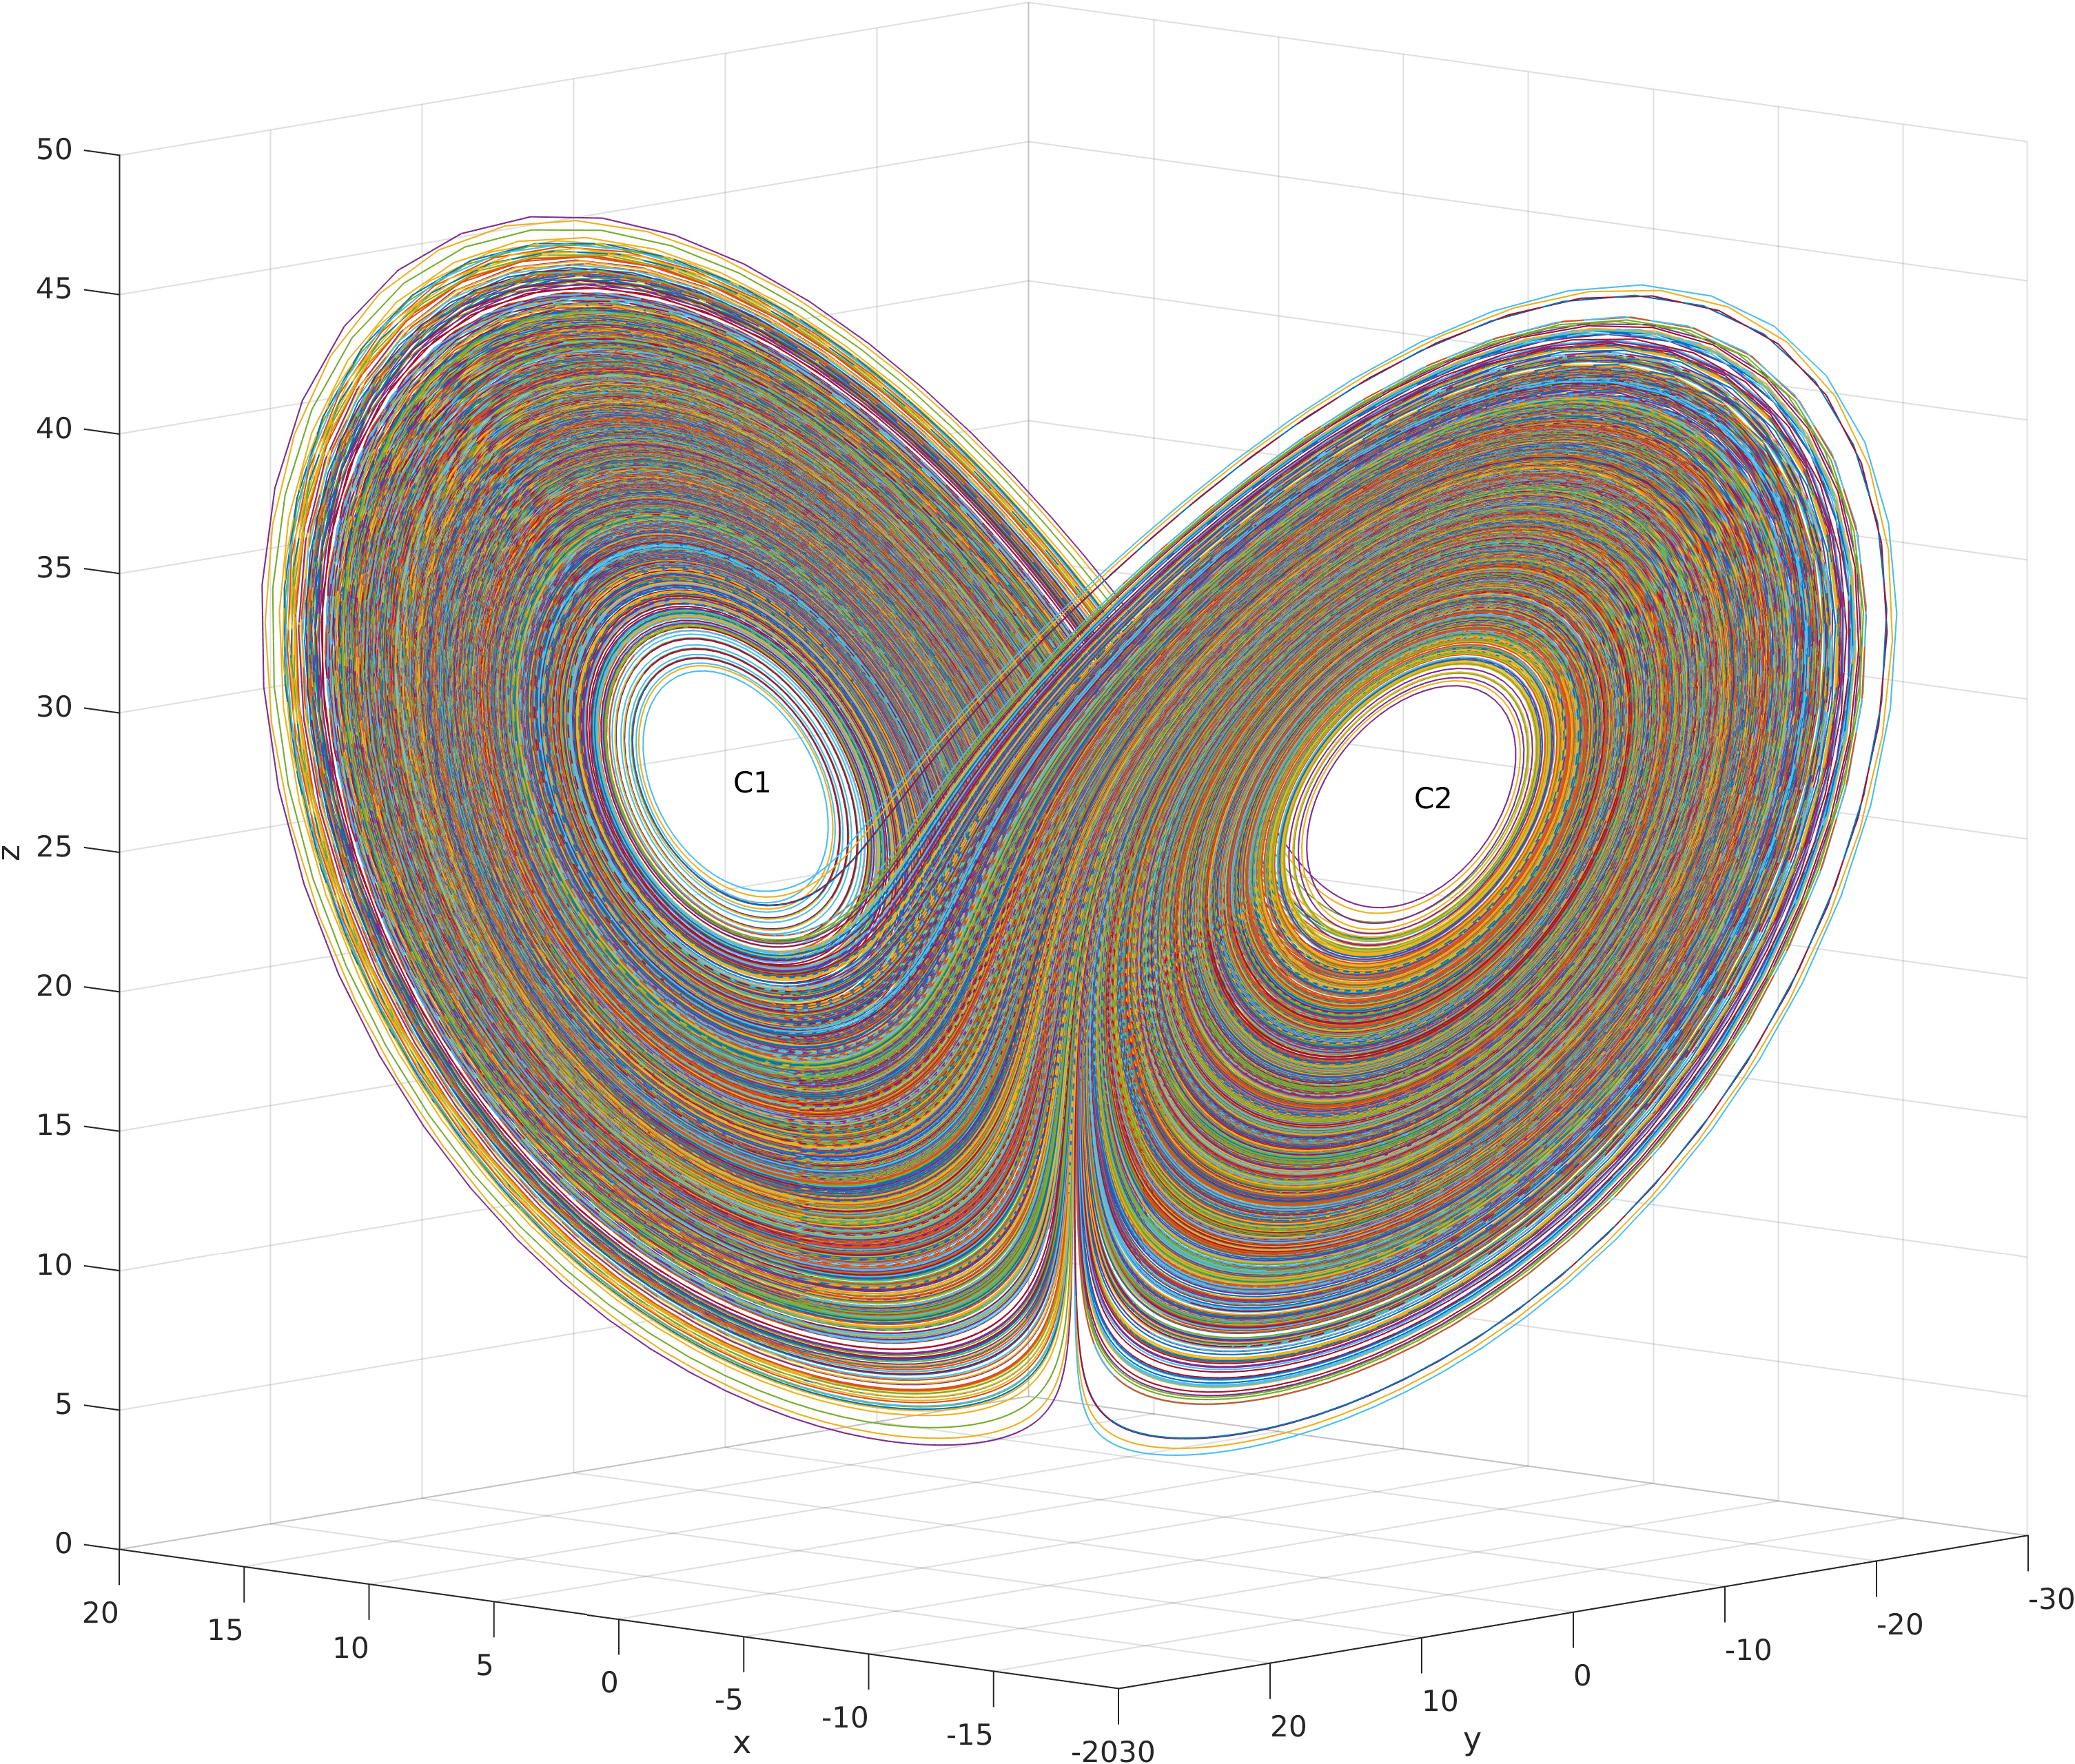
\includegraphics[width=0.9\textwidth]{attrattore-di-lorenz.png}
\vspace{1em}
\caption{Visualizzazione dell'attrattore di Lorenz.}
\label{fig:attrattore-di-lorenz}
\end{figure}

Per dare un'idea di tale sensibilità, abbiamo scelto due valori iniziali
\begin{equation} \label{eq:lorenz-valori-iniziali}
P_1 = (1,1,1)^T, \quad P_2 = (1+10^{-10},1,1)^T
\end{equation}
molto vicini tra loro, e abbiamo riportato nella Figura \ref{fig:lorenz-errore}
la distanza tra le traiettorie ad essi associate in funzione del tempo.
Si può osservare che, dopo un tratto iniziale in cui le soluzioni rimangono
a una distanza dell'ordine di $10^{-10}$, a partire da $t \approx 15$
la distanza comincia a crescere con velocità esponenziale, e questo comporta
una rapida separazione delle traiettorie che per $t = 40$ non hanno ormai più nulla
in comune (la distanza raggiunge infatti lo stesso ordine di grandezza del diametro
dell'attrattore di Lorenz).
Naturalmente, il fatto che un sistema dinamico sia così sensibile
alla scelta dei valori iniziali non è in sé niente di speciale: basti pensare
all'equazione test $y'(t) = \lambda y(t)$ con $\lambda > 0$, la cui simulazione
con dati iniziali \ref{eq:lorenz-valori-iniziali} dà lo stesso risultato
qualitativo della Figura \ref{fig:lorenz-errore} (a parte le regioni piatte
iniziali e finali). La cosa veramente sorprendente del sistema di Lorenz con $\rho = 28$
è che questo fenomeno si manifesta nel contesto di una dinamica \emph{dissipativa}
e \emph{contrattiva}, in cui le traiettorie non divergono all'infinito,
bensì convergono a una struttura di equilibrio comune.
Le implicazioni al di fuori della matematica sono enormi: se esistono
modelli matematici deterministici ma caotici, allora i fenomeni da essi
descritti non potranno essere oggetto di previsioni a lungo termine
(perché l'errore sui dati iniziali cresce esponenzialmente in funzione del tempo).
Per esempio, questo è il motivo per cui non si potranno mai avere delle previsioni
meteorologiche accurate a distanza di un mese, anche se avessimo a disposizione
modelli fluidodinamici perfetti e una potenza di calcolo illimitata.

Infine, osserviamo come gli errori di discretizzazione dovuti all'uso
di metodi numerici per la soluzione di equazioni differenziali siano
soggetti alla stessa amplificazione incontrollata degli errori sui dati
iniziali, quindi possiamo concludere che non esistono algoritmi stabili
per la soluzione di un problema ai valori iniziali in regime caotico
(anche perché, per quanto detto, è un problema il cui numero di condizionamento
è una funzione esponenziale dell'ampiezza dell'intervallo di simulazione).

\begin{figure}[tbp]
\centering
\begin{tikzpicture}[trim axis left, trim axis right]
\begin{semilogyaxis}[
	scale only axis,
	xlabel={$t$},
	xmin=-4,
	xmax=64,
	ylabel={Distanza tra le traiettorie},
	width=0.8\textwidth,
	height=0.5\textwidth,
]
\addplot[black] table[x=t, y=err] {lorenz.dat};
\end{semilogyaxis}
\end{tikzpicture}
\caption{Distanza tra le traiettorie con punti iniziali P1 e P2 in funzione del tempo.}
\label{fig:lorenz-errore}
\end{figure}

\section{Equazione logistica}

Nel corso di questo elaborato non abbiamo perso occasione per sottolineare
somiglianze e analogie tra sistemi dinamici continui e discreti.
Vediamo ora un'eccezione, cioè un sistema le cui dinamiche presentano
caratteristiche completamente diverse a seconda che sia formulato a tempo
continuo o a tempo discreto.

\subsection*{Il caso continuo}

Uno dei concetti di base della modellistica matematica è quello di
\emph{crescita esponenziale}, o \emph{crescita malthusiana}, in cui si
suppone che il tasso di crescita di una quantità $y(t)$ (ad esempio,
una popolazione) sia proporzionale alla quantità stessa:
\[
\left\{
\begin{aligned}
y'(t)  &= a y(t) \quad \text{per ogni $t \geq t_0$}, \\
y(t_0) &= y_0 > 0.
\end{aligned}
\right.
\qquad \qquad a > 0,
\]
Questo tipo di crescita, anche se molto comune, non può essere sostenuta
all'infinito: prima o poi nella dinamica di qualsiasi grandezza reale entrano
in gioco dei fattori interni o esterni che ne limitano la crescita.
Per esempio, nel caso di una popolazione umana, questi fattori possono essere
carestie, epidemie, guerre, cambiamenti socioculturali, ecc.
Un modello più realistico di crescita è dato quindi dall'\emph{equazione logistica}
\begin{equation} \label{eq:equazione-logistica-continua}
\left\{
\begin{aligned}
y'(t)  &= a y(t) - b y(t)^2 \quad \text{per ogni $t \geq t_0$}, \\
y(t_0) &= y_0 > 0,
\end{aligned}
\right.
\qquad \qquad a,b > 0,
\end{equation}
in cui $a$ continua a svolgere il ruolo di tasso di crescita, mentre il termine
$by(t)^2$ fa da freno alla crescita e porta $y'(t)$ ad assumere valori negativi
per $y(t)$ sufficientemente grande. Il problema \eqref{eq:equazione-logistica-continua}
si può scrivere nella forma equivalente
\[
\left\{
\begin{aligned}
y'(t)  &= a y(t) \left( 1 - \frac{y(t)}{y^*} \right) \quad \text{per ogni $t \geq t_0$}, \\
y(t_0) &= y_0 > 0,
\end{aligned}
\right.
\qquad \qquad y^* = \frac{a}{b},
\]
in cui il termine $1-y(t)/y^*$ è detto \emph{resistenza ambientale alla crescita}
e il termine $y^*$ è detto \emph{capacità portante}. Il motivo di quest'ultimo
nome è che $y^*$ è un punto di equilibrio globalmente asintoticamente stabile
per l'equazione logistica, e il modo più semplice di dimostrarlo è risolvere
direttamente il problema \eqref{eq:equazione-logistica-continua}
(è un caso particolare di equazione di Bernoulli):
\[
y(t) = \frac{y^* y_0 e^{a(t-t_0)}}{y^* + y_0 \left( e^{a(t-t_0)}-1 \right)}
\]
Dunque, per $t \to +\infty$ si ha che $y(t) \to y^*$ a prescindere dal valore
della condizione iniziale $y_0$ (a meno che $y_0 = 0$, ma si può dimostrare
che l'origine è un punto di equilibrio instabile).
Osserviamo infine che una crescita logistica con $y_0 \ll y^*$ presenta
due fasi distinte: finché $y < y^*/2$, il grafico di $y$ è convesso e la
crescita è molto vicina a quella esponenziale, mentre per valori di $y$
superiori a $y^*/2$ il grafico è concavo e la crescita si smorza convergendo
con velocità esponenziale all'asintoto orizzontale $y = y^* = a/b$.

\subsection*{Il caso discreto}

Lo stesso modello di crescita logistica può essere facilmente adattato al caso
discreto, in cui si suppone che le variazioni di una quantità $y$ non
avvengano in modo continuo, bensì a intervalli di tempo regolari:
\[
\left\{
\begin{aligned}
y_{n+1} &= a y_n - b y_n^2 \quad \text{per ogni $n \geq n_0$}, \\
y_{n_0} &= y_0 > 0,
\end{aligned}
\right.
\qquad \qquad a,b > 0.
\]
Tramite il cambio di variabile $z = (b/a)y$, possiamo scrivere questo problema
in una forma più semplice (con un piccolo abuso di notazione, manteniamo la
vecchia variabile $y$ al posto di $z$):
\begin{equation} \label{eq:equazione-logistica-discreta}
\left\{
\begin{aligned}
y_{n+1} &= a y_n (1-y_n) \quad \text{per ogni $n \geq n_0$}, \\
y_{n_0} &= y_0 > 0,
\end{aligned}
\right.
\qquad \qquad a > 0.
\end{equation}
Osserviamo che questo modello discreto, a differenza del caso continuo,
non è in grado di gestire valori di $y$ superiori a 1 (cioè, superiori a $a/b$ nella
variabile originale), altrimenti la successione $y_n$ inizierebbe ad assumere
valori negativi e il modello perderebbe di significato (ancora una volta,
si pensi al caso in cui $y_n$ rappresenta il numero di individui in una
popolazione al tempo $n$). Fortunatamente, questo problema può essere risolto
scegliendo $y_0 	\leq 1$ e ponendo una limitazione al tasso di crescita $a$:

\begin{teor}
Se $a \in [0,4]$, allora $y_0 \in [0,1]$ implica $y_n \in [0,1]$ per ogni $n \geq n_0$.
\end{teor}

\begin{proof}
Basta osservare che i valori della funzione $y \mapsto y(1-y)$ sull'intervallo $[0,1]$
sono compresi tra $0$ e $1/4$.
\end{proof}

\noindent In questo paragrafo andremo quindi a studiare le strutture di equilibrio
del problema \eqref{eq:equazione-logistica-discreta} al variare di $a$ in $[0,4]$.
Per quanto riguarda i punti di equilibrio, si ha che l'equazione
$\bar{y} = a \bar{y}(1-\bar{y})$ ha due sole soluzioni:
\[
\bar{y} = 0 \quad \text{e} \quad \bar{y} = \frac{a-1}{a}.
\]
Se $a \in [0,1]$, l'unico punto di equilibrio non negativo è l'origine,
e si dimostra facilmente che $\bar{y} = 0$ è globalmente asintoticamente stabile
perché $ay(1-y) < y$ per ogni $y > 0$.
Se $a > 1$, invece, l'origine diventa necessariamente instabile, perché
il sistema linearizzato in un intorno di zero è $y_{n+1} = a y_n$.
Se $a \in [1,3]$, la dinamica è globalmente attratta dall'altro punto di equilibrio,
mentre per $a > 3$ le cose si fanno più complesse: il punto $(a-1)/a$ diventa
instabile e gli insiemi di equilibrio non sono più singoli punti, bensì orbite
periodiche. Per valori di $a$ di poco superiori a~3 le traiettorie sono attratte
da un'orbita di periodo~2, ma al crescere di $a$ queste orbite di periodo~2
diventano instabili in favore di altre orbite di periodo~4, poi per
$a$ ancora maggiore quelle di periodo~4 diventano instabili in favore di altre
di periodo~8, e così via all'infinito. Questo fenomeno è detto \emph{cascata
di raddoppi del periodo}. Se indichiamo con $a_n$ il valore di $a$ in corrispondenza
del quale si verifica l'$n$-esimo raddoppio del periodo, cioè si passa da
orbite stabili di periodo $2^n$ a orbite stabili di periodo $2^{n+1}$, si
può dimostrare che la successione $a_n$ è convergente a un valore
$a_{\infty} \approx 3.57$ e che
\[
\lim_{n \to +\infty} \frac{a_n - a_{n-1}}{a_{n+1}-a_n} = \delta \approx 4.67.
\]
Questa costante $\delta$, detta \emph{numero di Feigenbaum}, non è specifica
dell'equazione logistica, ma si può ritrovare anche in altri sistemi dinamici
che presentano cascate di raddoppi del periodo come preludio a dinamiche
caotiche (per esempio, l'equazione di Lorenz con $\rho > 99$).

Se $a > a_\infty$ compaiono orbite stabili di periodo dispari, e a ognuna
di queste è associata una propria cascata di raddoppi del periodo.
Esistono dei valori di $a$ (ad esempio, $a = 3.83$) per cui si hanno
orbite periodiche stabili di periodo 3, e questo è stato dimostrato essere sufficiente
affinché la dinamica del sistema sia caotica. Infine, se $a = 4$, le traiettorie
sono completamente \emph{ergodiche}, cioè è stato dimostrato che per ogni insieme
di misura positiva $M \subseteq [0,1]$ si ha che per quasi ogni valore iniziale
$y_0$ il limite
\begin{equation} \label{eq:ergodicità-somma}
\lim_{n \to +\infty} \frac{1}{n} \sum_{i=1}^n \mathcal{X}_M(y_i)
\end{equation}
esiste finito ed è uguale all'integrale
\begin{equation} \label{eq:ergodicità-integrale}
\int_M \frac{1}{\pi \sqrt{y(1-y)}} \dy.
\end{equation}
Con $\mathcal{X}_M$ abbiamo indicato la funzione caratteristica dell'insieme $M$.
Si può dimostrare che la funzione integranda $h(y)$ sul dominio $[0,1]$
è una densità di probabilità invariante rispetto alla mappa logistica $y \mapsto 4y(1-y)$.
La proprietà di ergodicità della dinamica per $a=4$ è stata verificata
numericamente per mezzo del Programma \ref{prog:logistic-ergodicity},
la cui esecuzione ha prodotto il grafico nella Figura \ref{fig:logistic-ergodicity}.
Possiamo osservare un'ottima corrispondenza tra le
\emph{medie temporali}~\eqref{eq:ergodicità-somma} (raccolte in un istogramma)
e la densità $h(y)$ delle \emph{medie spaziali} \eqref{eq:ergodicità-integrale}
(disegnata senza gli asintoti verticali agli estremi del dominio).
Ricapitolando, la dinamica dell'equazione logistica discreta cambia moltissimo
al variare di $a$, al contrario dell'equazione logistica continua che per ogni
$a > 0$ presenta lo stesso identico andamento qualitativo.

\lstinputlisting[float=tbp, label=prog:logistic-ergodicity,
caption={Calcolo della distribuzione dei valori di $y_n$ per $a=4$.},
linerange={1-20}]{logistic_ergodicity.m}

\begin{figure}[tbp]
\centering
\includegraphics[height=0.4\textheight]{logistic-ergodicity.pdf}
\caption{Confronto tra medie temporali empiriche \eqref{eq:ergodicità-somma}
e media spaziale esatta \eqref{eq:ergodicità-integrale}.}
\label{fig:logistic-ergodicity}
\end{figure}

Per riassumere visivamente le strutture di equilibrio al variare di $a$ in $[0,4]$,
abbiamo scritto il Programma \ref{prog:logistic-bifurcation-diagram} che genera
il \emph{diagramma di biforcazione} dell'equazione logistica,
riportato in Figura \ref{fig:diagramma-di-biforcazione}.
In questo tipo di diagramma, a ogni pixel dell'immagine è associato un
valore di~$a$ (sulle ascisse, da 0 a 4) e un piccolo intervallo attorno
a un valore~$y$ (sulle ordinate, da 0 a 1).
Per generare una colonna dell'immagine (quindi, fissato $\bar{a}$) si sceglie
un valore iniziale $y_0$ e poi si effettuano due simulazioni consecutive
della dinamica: la prima per $N \gg 0$ passi in modo che $y_n$ sia attratto
dalla struttura di equilibrio attiva per $a = \bar{a}$, e la seconda per
altri $M \gg 0$ passi andando a marcare tutti i pixel dell'immagine a cui sono associati
degli intervalli che contengono almeno uno dei punti $y_{N+1},\dots,y_{N+M}$.
In questo modo, la colonna corrispondente a ogni valore di $a$ in un diagramma
di biforcazione fornisce una rappresentazione approssimativa della
struttura di equilibrio dell'equazione logistica $y_{n+1} = a y_n (1-y_n)$.

\lstinputlisting[float=tbp, label=prog:logistic-bifurcation-diagram,
caption={Calcolo del diagramma di biforcazione.}]{logistic_bifurcation_diagram.m}

\begin{figure}[tbp]
\centering
\begin{tikzpicture}[trim axis left, trim axis right]
\begin{axis}[
	enlargelimits=false,
	axis on top,
	xlabel={$a$},
	ylabel={$y$},
	width=0.9\textwidth,
	height=0.6\textwidth,
]
\addplot graphics [
	xmin=0,xmax=4,
	ymin=0,ymax=1,
] {bifurcation-diagram-edited.png};
\end{axis}
\end{tikzpicture}
\caption{Diagramma di biforcazione dell'equazione logistica discreta.}
\label{fig:diagramma-di-biforcazione}
\end{figure}

\begin{figure}[tbp]
\centering
\begin{tikzpicture}[trim axis left, trim axis right]
\begin{axis}[
	enlargelimits=false,
	axis on top,
	xlabel={$a$},
	ylabel={$y$},
	width=0.9\textwidth,
	height=0.9\textwidth,
]
\addplot graphics [
	xmin=3.5,xmax=4,
	ymin=0,ymax=1,
] {bifurcation-diagram-zoomed-edited.png};
\end{axis}
\end{tikzpicture}
\caption{Diagramma di biforcazione dell'equazione logistica discreta (dettaglio).}
\label{fig:diagramma-di-biforcazione-dettaglio}
\end{figure}

Nonostante la risoluzione limitata dell'immagine in Figura
\ref{fig:diagramma-di-biforcazione}, possiamo in effetti riconoscere il fenomeno
di raddoppio del periodo per valori di $a$ compresi tra 3 e 3.57.
Inoltre, l'aspetto della regione a destra di $a = 3.57$ lascia intuire la
complessità del regime caotico. La scelta del valore iniziale $y_0$ non è
particolarmente importante, perché quasi ogni valore viene attratto dalle
stesse strutture di equilibrio;
nella pratica la scelta $y_0 = 1/2$ funziona bene e converge rapidamente,
a parte il caso $a = 4$ in cui è uno dei punti dell'insieme di misura nulla
la cui dinamica non è ergodica (finisce in 0). Nel caso $a = 4$ abbiamo quindi
scelto $y_0 = 1/3$.




















\graphicspath{{./figures/capitolo8/}}
\lstset{inputpath = ./programs/capitolo8}
\pgfplotstableset{search path = ./tables/capitolo8}

\chapter{Metodi Runge-Kutta}

In quest'ultimo capitolo torneremo ad occuparci di metodi numerici
per la discretizzazione del problema di Cauchy
\begin{equation} \label{eq:problema-di-cauchy-cap8}
\left\{
\begin{aligned}
y'(t)  &= f(t,y(t)) \quad \text{per ogni $t \in [t_0,T]$}, \\
y(t_0) &= y_0 \in \R^m,
\end{aligned}
\right.
\end{equation}
e vedremo come, attraverso l'introduzione di metodi numerici più flessibili,
sarà possibile superare la seconda barriera di Dahlquist e allo stesso
tempo trattare in modo qualitativamente corretto non solo problemi dissipativi,
ma anche problemi conservativi di tipo hamiltoniano (si parla in questo caso
di integratori geometrici). Nel Capitolo 3, l'idea alla base dei metodi numerici
multistep era quella di discretizzare direttamente l'equazione differenziale
\eqref{eq:problema-di-cauchy-cap8} tramite un'opportuna equazione alle differenze;
in questo capitolo vedremo invece un approccio basato sulla forma integrale
dell'equazione \eqref{eq:problema-di-cauchy-cap8}. Sia
$t_0 < t_1 < \dots t_N = T$ una partizione dell'intervallo $[t_0,T]$,
non per forza uniforme. Allora, a ogni passo temporale discreto
possiamo scrivere che
\[
y(t_{n+1}) = y(t_n) + \int_{t_n}^{t_{n+1}} f(t,y(t)) \dt.
\]
Come nel Capitolo 3, indichiamo con $y_n$ l'approssimazione di $y(t_n)$
fornita dal metodo numerico e con $h$ l'incremento temporale $t_{n+1}-t_n$.
Per discretizzare l'integrale dell'equazione precedente possiamo ricorrere
a una formula di quadratura con $s$ nodi
\[
t_n + c_1 h,\, \dots,\, t_n + c_s h \qquad 0 \leq c_1 \leq \dots \leq c_s \leq 1
\]
e con pesi $b_1, \dots, b_s$:
\vspace{-1em}
\begin{equation} \label{eq:sistema-yn+1-runge-kutta}
y_{n+1} = y_n + h \sum_{i=1}^s b_i f(t_n+c_i h, y(t_n + c_i h)).
\end{equation}
Il valore $s$ è detto \emph{numero di stadi} del metodo.
A questo punto, rimane solo da decidere come approssimare i valori
$y(t_n+c_i h)$ (tali approssimazioni verranno indicate con $Y_i$).
L'idea alla base dei \emph{metodi Runge-Kutta} è quella di ricorrere
nuovamente al teorema fondamentale del calcolo
\[
y(t_n + c_i h) = y(t_n) + \int_{t_n}^{t_n+c_i h} f(t,y(t)) \dt,
\]
e di approssimare anche questi nuovi integrali con delle formule
di quadratura basate sugli stessi nodi $c_1, \dots, c_s$ e con pesi $a_{ij}$:
\begin{equation} \label{eq:sistema-Yi-runge-kutta}
Y_i = y_n + h \sum_{j=1}^s a_{ij} f(t_n + c_j h, Y_j).
\end{equation}
In questo modo, la \eqref{eq:sistema-yn+1-runge-kutta} e la
\eqref{eq:sistema-Yi-runge-kutta} formano un sistema chiuso di $s+1$ equazioni
vettoriali nelle incognite $Y_1,\dots,Y_s,y_{n+1}$, la cui soluzione
ci permette di avanzare nel tempo di una quantità $h = t_{n+1}-t_n$.
I coefficienti $a_{ij}$ formano una matrice $A$ detta \emph{matrice di Butcher},
mentre i coefficienti $b_i$ e $c_i$ formano dei vettori $b$ e $c$ detti
rispettivamente \emph{vettore dei pesi} e \emph{vettore dei nodi}.
La terna $(A,b,c)$ caratterizza in modo univoco il particolare metodo Runge-Kutta
e solitamente viene riportata sotto forma di \emph{tableau di Butcher}
\[
\renewcommand\arraystretch{1.4}
\begin{array}
{c|c}
c & A \\
\hline
 & b^{\mathrlap{\scriptscriptstyle T}} \\
\end{array}
\]
Osserviamo che, a differenza dei metodi lineari multistep, i metodi Runge-Kutta
sono metodi a un solo passo, perché $y_{n+1}$ dipende unicamente da $y_n$
e non dai valori $y_i$ precedenti.

Anche in questo contesto, ha senso distinguere tra metodi espliciti e metodi
impliciti. Se la matrice $A$ è strettamente triangolare inferiore, le
equazioni \eqref{eq:sistema-Yi-runge-kutta} possono essere risolte
al variare di $i = 1,\dots,s$ tramite delle semplici sostituzioni in avanti,
quindi la complessità computazionale di ogni passo è bassa (pari a $O(m)$)
e per questo si parla di \emph{metodo Runge-Kutta esplicito}.
Se invece $A$, pur essendo triangolare inferiore, ha elementi non nulli
sulla diagonale, allora l'equazione \eqref{eq:sistema-Yi-runge-kutta} diventa
\[
Y_i - ha_{ii}f(t_n+c_i h,Y_i)
= y_n + h \sum_{j=1}^{i-1} a_{ij} f(t_n + c_j h, Y_j)
\eqd g_n,
\]
e in questo caso si parla di \emph{metodo Runge-Kutta semi-implicito}.
Osserviamo che ogni equazione nonlineare \eqref{eq:sistema-Yi-runge-kutta}
può essere risolta separatamente, purché lo si faccia nell'ordine giusto,
e che sotto l'ipotesi $h \abs{a_{ii}} L < 1$ la soluzione $Y_i$
di ciascuna equazione esiste ed è unica per il teorema di punto fisso di Banach.
Infine, se $A$ ha elementi non nulli al di sopra della diagonale, le $s$
equazioni \eqref{eq:sistema-Yi-runge-kutta} formano necessariamente un
unico sistema nonlineare di $sm$ equazioni scalari che non può essere
a priori semplificato. Almeno la notazione, però, può essere resa più compatta:
siano $\otimes$ il prodotto di Kronecker tra matrici e $Y,f(Y),e$
i vettori colonna
\[
Y = \begin{pmatrix}
Y_1 \\ 
\vdots \\ 
Y_s \\
\end{pmatrix} \in \R^{sm}, \quad
f(Y) = \begin{pmatrix}
f(t_n+c_1 h, Y_1) \\ 
\vdots \\ 
f(t_n+c_s h, Y_s) \\
\end{pmatrix} \in \R^{sm}, \quad
e = \begin{pmatrix}
1 \\ 
\vdots \\ 
1 \\
\end{pmatrix} \in \R^{s}.
\]
Allora il sistema delle equazioni \eqref{eq:sistema-Yi-runge-kutta} corrisponde a
\[
F(Y) \deq Y - e \otimes y_n - h (A \otimes I_m) f(Y) = 0.
\]
In questo caso si parla di \emph{metodo Runge-Kutta implicito}, e si può
dimostrare che l'ipotesi giusta per applicare il teorema di punto fisso
di Banach è $h \norm{A} L < 1$.
Nella pratica computazionale, ha senso distinguere i metodi semi-impliciti
da quelli impliciti, perché c'è un vantaggio non trascurabile nel risolvere
$s$ sistemi di dimensione $m$ rispetto a un solo sistema di dimensione $sm$.

Come nel caso dei metodi lineari multistep, ci sono buoni motivi per evitare
di risolvere i sistemi non lineari mediante iterazioni di punto fisso.
La matrice jacobiana di $F(Y)$, necessaria per poter impiegare
il metodo di Newton o una delle sue varianti, è la seguente:
\[
F'(Y) = I_{sm} - h (A \otimes I_m) \begin{pmatrix}
\partial_y f(t_n+c_1 h,Y_1) & & \\
& \ddots & \\
& & \partial_y f(t_n+c_s h,Y_s) \\
\end{pmatrix}.
\]
Nel caso del metodo di Newton stazionario, l'unica jacobiana di $f$ da calcolare
a ogni passo sarà $J_0 = \partial_y f(t_n,y_n) \approx \partial_y f(t_n+c_i h, Y_i)$,
quindi l'espressione precedente può essere semplificata:
\[
F'(Y) \approx I_{sm} - h (A \otimes I_m)(I_s \otimes J_0) = I_{sm} - h (A \otimes J_0).
\]
A conclusione di questo paragrafo, riportiamo il Programma \ref{prog:runge-kutta},
che illustra una possibile implementazione di un generico metodo Runge-Kutta
in funzione dei coefficienti $(A,b,c)$. Possiamo osservare le numerose
somiglianze a livello di scelte implementative con l'analogo
Programma \ref{prog:lmf} del Capitolo 3, che illustrava un generico metodo
lineare multistep. I sistemi non lineari nel caso semi-implicito e implicito
sono risolti dai Programmi \ref{prog:RK-semiimplicit-solver} e
\ref{prog:RK-implicit-solver} utilizzando il metodo di Newton stazionario.
La funzione \code{numerical\_jacobian} è la stessa del Capitolo 3
(Programma \ref{prog:lmf-numerical-jacobian}).

\clearpage

\lstinputlisting[label=prog:runge-kutta, caption={Implementazione
di un generico metodo Runge-Kutta.}]{runge_kutta.m}

\lstinputlisting[float=p, label=prog:RK-semiimplicit-solver, caption={Metodo di Newton
stazionario per metodi Runge-Kutta semi-impliciti.}]{RK_semiimplicit_solver.m}

\lstinputlisting[float=p, label=prog:RK-implicit-solver, caption={Metodo di Newton
stazionario per metodi Runge-Kutta impliciti.}, linerange={1-6,10-31}]{RK_implicit_solver.m}

\clearpage

\section{Proprietà dei metodi Runge-Kutta}

Per quanto riguarda le proprietà dei metodi Runge-Kutta, valgono definizioni
del tutto analoghe a quelle date per i metodi lineari multistep, anche se
qui preferiamo non riportare i dettagli: si può dunque parlare di ordine
di convergenza, di errore di troncamento locale, di consistenza, di zero-stabilità
e di assoluta stabilità. %anche in questo contesto

Consideriamo il problema $y'(t) = 0$, $y(t_0) = y_0$ associato all'analisi
di zero-stabilità di un metodo numerico per equazioni differenziali ordinarie.
Dato che $f(t,y) \equiv 0$, è immediato verificare che l'equazione
\[
y_{n+1} = y_n + h \sum_{i=1}^s b_i f(t_n+c_i h, Y_i)
\]
con cui un generico metodo Runge-Kutta avanza nel tempo si semplifica in
$y_{n+1} = y_n$, quindi possiamo concludere che i metodi Runge-Kutta
sono incondizionatamente zero-stabili.
Allora, dato che anche per i metodi Runge-Kutta si può dimostrare un risultato
analogo al Teorema \ref{teor:ordine-convergenza-lmf}, cioè che consistenza
e zero-stabilità sono condizioni sufficienti per la convergenza, si ha che
la classe dei metodi Runge-Kutta convergenti coincide con quella
dei metodi Runge-Kutta consistenti.
La condizione sui coefficienti $(A,b,c)$ di un metodo Runge-Kutta che caratterizza
la consistenza è
\[
\sum_{i=1}^s b_i = 1,
\]
ma a differenza dei metodi lineari multistep non esiste una caratterizzazione
dei metodi di ordine superiore semplice come quella del Teorema \ref{teor:ordine-lmf}:
i vincoli che si ottengono dalla formula di Taylor non sono lineari, non sono
tutti indipendenti e crescono in numero molto velocemente in funzione
dell'ordine $p$.
Per questo motivo teoremi come l'\ref{teorema-ordine-convergenza-HBVM},
che vedremo a breve, svolgono un ruolo importante all'interno della teoria
di questi metodi.

Per quanto riguarda l'assoluta stabilità, l'equazione
\eqref{eq:sistema-yn+1-runge-kutta} applicata all'equazione test scalare
$y'(t) = \lambda y(t)$ fornisce l'equazione lineare
\[
y_{n+1} = y_n + h \sum_{i=1}^s b_i \lambda Y_i = y_n + h \lambda b^T Y,
\]
mentre l'equazione \eqref{eq:sistema-Yi-runge-kutta} fornisce
\[
Y = e \otimes y_n + h (A \otimes I_1) \lambda Y
= e y_n + h \lambda A Y
\eqd e y_n + q A Y.
\]
Mettendo insieme queste due equazioni, otteniamo il sistema lineare
\[
\begin{pmatrix}
I-qA   & 0 \\ 
-q b^T & 1 \\
\end{pmatrix}
\begin{pmatrix}
Y       \\
y_{n+1} \\
\end{pmatrix}
= \begin{pmatrix}
e y_n \\
y_n   \\
\end{pmatrix},
\]
la cui soluzione si può esprimere per mezzo della regola di Cramer:
\begin{equation} \label{eq:funzione-di-stabilità}
y_{n+1} = \frac{\det(I-qA+qeb^T)}{\det(I-qA)} y_n \eqd R(q) y_n.
\end{equation}
La funzione $R(q)$ è detta \emph{funzione di stabilità} del metodo Runge-Kutta
e si può dimostrare che $R(q)$ è una funzione razionale della variabile $q = h\lambda$.
Dato che $y_n = R(q)^n y_0$, la regione di assoluta stabilità $\mathcal{D}$ è definita
come l'insieme dei valori $q \in \C$ tali che $\abs{R(q)} < 1$. Anche in questo
caso, si può dimostrare che tutti i metodi espliciti hanno necessariamente una regione
di assoluta stabilità limitata, quindi dovremo ricorrere a metodi (semi)impliciti
ogniqualvolta sia richiesta l'assoluta stabilità.
A differenza dei metodi lineari multistep, invece, esistono metodi A-stabili
(addirittura, perfettamente A-stabili) di ordine arbitrariamente elevato,
come vedremo in seguito. Prima, però, riassumiamo brevemente vantaggi e svantaggi
nell'utilizzo dei metodi Runge-Kutta rispetto ai metodi lineari multistep.
Cominciamo dai vantaggi:
\begin{itemize}
\item I metodi Runge-Kutta sono incondizionatamente zero-stabili.
\item I metodi Runge-Kutta non richiedono il calcolo di $k-1$ valori iniziali
mancanti, tant'è che alcune implementazioni di metodi lineari multistep vengono
avviate mediante metodi a un passo come i Runge-Kutta.
\item I metodi Runge-Kutta non sono soggetti alla seconda barriera di Dahlquist,
che limita l'ordine di convergenza dei metodi A-stabili. In generale, possiamo
dire che i metodi Runge-Kutta sono più ricchi e flessibili dei metodi lineari multistep.
\item I metodi Runge-Kutta permettono di gestire facilmente il caso in cui
i passi temporali $h$ non sono uniformi, quindi sono più indicati per sviluppare
metodi adattativi (come \code{ode45} di MATLAB).
\end{itemize}
Per quanto riguarda gli svantaggi,
\begin{itemize}
\item I metodi lineari a $k$ passi, a parità di ordine, richiedono meno
valutazioni di $f$, perché i valori $f_n$ possono essere utilizzati per $k$
passi consecutivi. I metodi Runge-Kutta, invece, calcolano i valori
$Y_i \approx y(t_n+c_i h)$ a ogni passo, e poi scartano queste informazioni
all'inizio del passo successivo.
\item L'analisi delle proprietà dei metodi lineari multistep è più semplice
(in particolare, lo studio dell'ordine di un dato metodo).
\item I metodi lineari a $k$ passi impliciti richiedono a ogni passo
la soluzione di un solo sistema non lineare di dimensione $m$ a prescindere
da $k$, mentre i metodi Runge-Kutta impliciti richiedono la soluzione di $s$
sistemi non lineari di dimensione $m$, o di un sistema di dimensione $sm$.
Dunque, solo per i metodi Runge-Kutta il costo computazionale aumenta in maniera
significativa al crescere dell'ordine del metodo stesso.
\end{itemize}

\section{Regione di assoluta stabilità del metodo RK classico}

Uno dei metodi Runge-Kutta più utilizzati nelle applicazioni è quello
definito dal tableau di Butcher
\[
\renewcommand\arraystretch{1.4}
\begin{array}
{c|cccc}
0   & 0   &     &   &   \\
1/2 & 1/2 & 0   &   &   \\
1/2 & 0   & 1/2 & 0 &   \\
1   & 0   & 0   & 1 & 0 \\
\hline
    & 1/3 & 1/6 & 1/6 & 1/3 \\
\end{array}
\]
\\
detto \emph{metodo Runge-Kutta classico}. La sparsità della matrice $A$
rende infatti piuttosto semplice implementare questo metodo, e la bassa
complessità computazionale che ne deriva ne ha reso possibile l'utilizzo
fin da prima dell'avvento del calcolatore elettronico (il metodo risale infatti
al 1901, e si deve al matematico tedesco Martin Kutta).
Si può dimostrare che il metodo è del quarto ordine, quindi ha buone proprietà
di convergenza, anche se le proprietà di stabilità lasciano inevitabilmente
a desiderare: essendo un metodo esplicito, la sua regione di assoluta stabilità
è limitata. In teoria, la formula \eqref{eq:funzione-di-stabilità} permette
di descrivere tale regione in forma chiusa sotto forma di disuguaglianza,
ma non è facile poi trasformare questa rappresentazione in una forma più
comprensibile (né esiste un equivalente del boundary locus nell'ambito dei
metodi Runge-Kutta).

\lstinputlisting[float=p, label=prog:plot-stability-region,
linerange={1-10}, caption={Calcolo della regione di assoluta stabilit\`{a}
del metodo Runge-Kutta classico.}]{plot_stability_region.m}

\lstinputlisting[float=p, label=prog:is-in-stability-region, caption={Test di
appartenenza alla regione di assoluta stabilit\`{a} di un metodo Runge-Kutta.}] {is_in_stability_region.m}

\begin{figure}[p]
\centering
\includegraphics[height=0.35\textheight]{regione-RK-classico.png}
\caption{Regione di assoluta stabilità del metodo Runge-Kutta classico.}
\label{fig:regione-RK-classico}
\end{figure}

Per questo motivo, abbiamo scritto il Programma \ref{prog:plot-stability-region},
che disegna in modo approssimato la regione di assoluta stabilità del metodo
Runge-Kutta classico tramite un approccio di forza bruta basato su una griglia
regolare (la posizione e la dimensione della griglia sono state scelte a posteriori
in modo da ricoprire $\mathcal{D}$).
In ogni punto $q$ della griglia, il Programma \ref{prog:is-in-stability-region}
permette di stabilire se $q$ appartenga o meno a $\mathcal{D}$,
dopodiché la funzione \code{contourf} di MATLAB (basata sull'algoritmo
\emph{marching squares}) disegna sulla griglia un'approssimazione lineare a tratti
delle curve di livello della funzione caratteristica
dei punti $q$ interni a $\mathcal{D}$. La risoluzione dell'immagine risultante
(Figura \ref{fig:regione-RK-classico}) è pertanto la stessa della griglia,
che in questo esempio abbiamo scelto 500x500. Osserviamo che, se $\lambda \in \R^-$,
la restrizione sul passo $h$ affinché $q \in \mathcal{D}$ è circa $h \abs{\lambda} < 2.8$.

\section{Hamiltonian Boundary Value Methods}

Vediamo ora metodi numerici in grado di fornire discretizzazioni qualitativamente
corrette non solo nel caso dissipativo, ma anche nel caso conservativo.
Concentriamo l'attenzione su un particolare intervallo di tempo discreto
$[t_n,t_{n+1}]$, e cerchiamo un polinomio $u(t_n+ch)$ di grado $s$ che
approssimi la soluzione esatta $y(t_n+ch)$ per $c \in [0,1]$.
Dato che i polinomi di Legendre $P_j(c)$ shiftati e normalizzati
sull'intervallo $[0,1]$ formano un sistema ortonormale completo in $L^2([0,1])$,
sotto le dovute ipotesi di regolarità la derivata della soluzione $y'(t_n+ch)$
è uguale alla propria serie di Fourier rispetto alla base $\{P_j\}_{j \in \N}$:
\[
y'(t_n+ch) = \sum_{j=0}^{+\infty} \gamma_j P_j(c), \quad
\text{con } \gamma_j = \int_0^1 y'(t_n+ch) P_j(c) \dc
= \int_0^1 f(y(t_n+ch)) P_j(c) \dc.
\]
Da qui, l'idea degli \emph{Hamiltonian Boundary Value Methods} è quella di
cercare un polinomio $u(t_n+ch)$ che soddisfi una versione discreta e
finito-dimensionale dell'equazione precedente:
\begin{equation} \label{eq:discretizzazione-serie-di-fourier}
u'(t_n+ch) = \sum_{j=0}^{s-1} \hat{\gamma_j} P_j(c), \quad
\text{con } \hat{\gamma_j} = \sum_{\ell=1}^k b_\ell f(u(t_n + c_\ell h)) P_j(c_\ell)
\end{equation}
La serie di Fourier è stata dunque troncata dopo $s$ termini, mentre l'integrale
sull'intervallo $[0,1]$ è stato approssimato mediante formula di quadratura
su $k$ nodi $c_1,\dots,c_k$ con pesi $b_1,\dots,b_k$.
Sia $y_n$ l'approssimazione di $y(t_n)$ a ogni passo del metodo numerico.
Allora, la condizione $u(t_n) = y_n$ e le $s$ condizioni scalari sulla derivata
di $u(t_n+ch)$ determinano in modo univoco il polinomio $u \in \Pi_s$ cercato,
il cui valore in $t_{n+1}$ fornisce la nuova approssimazione $y_{n+1} \approx y(t_{n+1})$:
\begin{gather*}
\int_0^1 u'(t_n+ch) \dc
= \int_0^1 \, \sum_{j=0}^{s-1} \hat{\gamma_j} P_j(c) \dc
\qquad u(t_{n+1}) - u(t_n)
= h \int_0^1 \, \sum_{j=0}^{s-1} \hat{\gamma_j} P_j(c) \dc \\
y_{n+1}
= y_n + h \sum_{j=0}^{s-1} \hat{\gamma_j} \int_0^1 \! P_j(c) \dc
= y_n + h \hat{\gamma_0}
= y_n + h \sum_{\ell=1}^k b_\ell f(u(t_n+c_\ell h)).
\end{gather*}
Vista la somiglianza di questa equazione con la \eqref{eq:sistema-yn+1-runge-kutta}
(anche se qui, per semplicità, siamo nel caso omogeneo), chiamiamo $Y_i$
i valori $u(t_n + c_i h)$ al variare di $i = 1,\dots,k$ e integriamo nuovamente
la \eqref{eq:discretizzazione-serie-di-fourier}, stavolta da $0$ a $c_i$:
\begin{gather*}
\int_0^{c_i} u'(t_n+ch) \dc
= \int_0^{c_i} \, \sum_{j=0}^{s-1} \hat{\gamma_j} P_j(c) \dc
\qquad u(t_n + c_i h) - u(t_n)
= h \int_0^1 \, \sum_{j=0}^{s-1} \hat{\gamma_j} P_j(c) \dc \\
Y_i
= y_n + h \sum_{j=0}^{s-1} \hat{\gamma_j} \int_0^{c_i} \! P_j(c) \dc
= y_n + h \sum_{j=0}^{s-1}
	\left( \sum_{\ell=1}^k b_\ell f(Y_\ell) P_j(c_\ell) \right)
	\! \int_0^{c_i} \! P_j(c) \dc \\
= y_n + h \sum_{\ell=1}^k
	\left( \sum_{j=0}^{s-1} \int_0^{c_i} \! P_j(c) \dc \, P_j(c_\ell) b_\ell \right)
	f(Y_\ell)
\eqd y_n + h \sum_{\ell=1}^k a_{i\ell} f(Y_\ell)
\end{gather*}
Abbiamo pertanto ottenuto un metodo Runge-Kutta a $k$ stadi, detto
\emph{Hamiltonian Boundary Value Method $(k,s)$} e solitamente abbreviato in HBVM($k,s$).
Si può dimostrare che la matrice di Butcher $A$ è uguale a
$\mathcal{I}_s \mathcal{P}_s \Omega$, con
\begin{gather*}
\mathcal{I}_s = \begin{pmatrix}
\int_0^{c_1} \! P_{0}(c) \dc & \hdots & \int_0^{c_1} \! P_{s-1}(c) \dc \\ 
\vdots & & \vdots \\ 
\int_0^{c_k} \! P_{0}(c) \dc & \hdots & \int_0^{c_k} \! P_{s-1}(c) \dc
\end{pmatrix},
\quad \mathcal{P}_s = \begin{pmatrix}
P_0(c_1) & \hdots & P_{s-1}(c_1) \\
\vdots & & \vdots \\
P_0(c_k) & \hdots & P_{s-1}(c_k)
\end{pmatrix},
\quad \Omega = \begin{pmatrix}
b_1 & & \\
& \ddots & \\
& & b_k
\end{pmatrix}.
\end{gather*}
Oltre ai parametri $k$ e $s$, a definire un metodo HBVM è anche la scelta della
particolare formula di quadratura con cui vengono approssimati i coefficienti
di Fourier
\[
\gamma_j = \int_0^1 f(u(t_n+ch)) P_j(c) \dc.
\]
Una scelta molto buona, per certi versi ottima, è quella della formula di
quadratura di Gauss-Legendre, perché ha ordine massimo $2k$ tra
tutte le formule di quadratura di tipo interpolatorio su $k$ nodi.
Per questo, adotteremo tale scelta per tutto il resto del capitolo.
Dunque, $c_i$ sarà l'$i$-esima radice del polinomio di Legendre $P_k$,
e $b_i$ sarà l'integrale da 0 a 1 dell'$i$-esimo polinomio della base
di Lagrange definita sulle ascisse $c_1,\dots,c_k$. Sotto queste ipotesi,
si può dimostrare che i metodi HBVM($k,s$) hanno ordine $2s$ e sono
perfettamente A-stabili:

\begin{teor} \label{teorema-ordine-convergenza-HBVM}
Se $y_n = y(t_n)$ e $k \geq s$, allora l'approssimazione $y_{n+1}$ fornita
dal metodo HBVM($k,s$) soddisfa $y_{n+1}-y(t_{n+1}) = O(h^{2s+1})$.
In altre parole, il metodo HBVM($k,s$) ha errore di troncamento locale
dell'ordine di $h^{2s+1}$.
\end{teor}

\begin{teor}
Se $k \geq s$, la regione di assoluta stabilità del metodo HBVM($k,s$) è $\C^-$.
\end{teor}

\noindent Come anticipato, possiamo concludere che per i metodi Runge-Kutta
non vale un risultato analogo alla seconda barriera di Dahlquist
\ref{teor:seconda-barriera-dahlquist}.

\section{Problemi hamiltoniani}

Osserviamo che, da un punto di vista formale, i metodi HBVM($k,s$) sono metodi
Runge-Kutta a $k$ stadi, tuttavia il loro ordine di convergenza è funzione di $s$,
e questo non è sorprendente perché stiamo pur sempre approssimando $y(t)$
con un polinomio $u(t)$ di grado $s$, non $k$.
Ma, allora, perché non scegliere sempre $s=k$?
I motivi sono sostanzialmente due, e hanno a che fare con la soluzione
di problemi conservativi, di tipo hamiltoniano:

\begin{defi}
Si dice \emph{problema hamiltoniano} un problema della forma
\begin{equation} \label{eq:problema-hamiltoniano-qp}
\left\{
\begin{aligned}
q'(t)  &= \partial_p H (q(t),p(t)) \quad \text{per ogni $t \in [t_0,T]$}, \\
p'(t)  &= - \partial_q H (q(t),p(t)) \quad \text{per ogni $t \in [t_0,T]$}, \\
q(t_0) &= q_0 \in \R^m, \quad p(t_0) = p_0 \in \R^m,
\end{aligned}
\right.
\end{equation}
con $H(q,p) \colon \R^m \times \R^m \to \R^m$ funzione differenziabile
detta \emph{hamiltoniana}.
\end{defi}

\noindent Il caso del moto di una particella di massa $M$ in un campo
di forze conservative in $\R^m$ con potenziale $U$
\[
q''(t) = -\grad U(q) \in \R^m
\]
è un esempio di problema hamiltoniano con
\[
H(q,p) = \frac{1}{2M} \norm{p}^2 + U(q),
\]
infatti $q'(t) = p(t)/M$, $p'(t) = -\grad U(q(t))$.
Il problema \eqref{eq:problema-hamiltoniano-qp} può essere scritto in forma
più compatta nell'incognita $y(t) = (q(t),p(t))^T$ nel modo seguente:
\begin{equation*} \label{eq:problema-hamiltoniano-y}
\left\{
\begin{aligned}
y'(t)  &= J \grad H (y(t)) \quad \text{per ogni $t \in [t_0,T]$}, \\
y(t_0) &= y_0 = (q_0,p_0) \in \R^{2m},
\end{aligned}
\right.
\quad J = \begin{pmatrix}
0 & I_m \\ 
-I_m & 0
\end{pmatrix},
\quad \grad H(y) = \begin{pmatrix}
\partial_q H(y) \\ 
\partial_p H(y)
\end{pmatrix} 
\end{equation*}
Il valore dell'hamiltoniana $H(y)$ è un invariante lungo il moto di ogni sistema
hamiltoniano, infatti
\[
\frac{d}{dt} H(y(t)) = \grad H (y(t))^T J \grad H(y(t)) = 0,
\]
perché $J$ è una matrice antisimmetrica. Abbiamo dunque un'importante proprietà
qualitativa del moto che vorremmo preservare nel processo di discretizzazione
dell'equazione differenziale. In effetti, questa è la ragion d'essere
dei metodi HBVM e il primo dei due motivi per cui ha senso scegliere $k > s$:

\begin{teor}
Discretizzando un sistema hamiltoniano con un metodo HBVM($k,s$) con $k \geq s$
si ha che $H(y_{n+1}) - H(y_n) = O(h^{2k+1})$.
\end{teor}

\noindent Come corollario, si dimostra facilmente per mezzo della disuguaglianza
triangolare che
\[
\max_{0 \leq n \leq N} \Bigl\lbrace \abs{H(y_n)-H(y_0)} \Bigr\rbrace
= O(h^{2k}), \quad \text{con $N = (T-t_0)h^{-1}$.}
\]
Allora, è sufficiente scegliere $k$ tale che
$h^{2k} \approx \varepsilon = 1.1 \cdot 10^{-16}$ per avere
una conservazione \emph{pratica} dell'hamiltoniana,
cioè una conservazione non \emph{esatta}, ma entro i limiti della
precisione di macchina (meglio di così non si può fare, né c'è veramente
bisogno di farlo). Osserviamo che questa proprietà di conservazione dell'hamiltoniana
è indipendente dall'ordine $2s$ del metodo, anche se, a parità di
ordine di convergenza, i metodi conservativi hanno senz'altro un errore
più piccolo.

Il secondo motivo per cui ha senso scegliere $k > s$ è che, nonostante
il metodo HBVM($k,s$) sia da un punto di vista formale un metodo Runge-Kutta
a $k$ stadi, non è strettamente necessario risolvere il sistema non lineare
\[
F(Y) = Y - e \otimes y_n - h(A \otimes I_{2m}) f(Y)
\]
di dimensione $2mk$: il polinomio $u$ ha grado $s$ e quindi è inutile andare
a calcolare i suoi valori $Y_i = u(t_n + c_i h)$ in $k > s$ punti distinti.
Cambiamo allora punto di vista, e cerchiamo di ottenere un sistema chiuso
di equazioni per gli $s$ coefficienti di Fourier $\hat{\gamma_j} \in \R^{2m}$:
\begin{gather}
\hat{\gamma_j}
= \sum_{\ell=1}^k b_\ell f(u(t_n + c_\ell h)) P_j(c_\ell)
\qquad u(t_n + c_\ell h)
= y_n + h \sum_{j=0}^{s-1} \hat{\gamma_j} \int_0^{c_\ell} \! P_j(c) \dc \\
\label{eq:sistema-gamma-runge-kutta}
\hat{\gamma_j}
= \sum_{\ell=1}^k b_\ell \, f \left(
	y_n + h \sum_{i=0}^{s-1} \hat{\gamma_i} \int_0^{c_\ell} \! P_i(c) \dc
	\right) P_j(c_\ell)
\end{gather}
Le equazioni non lineari \eqref{eq:sistema-gamma-runge-kutta} al variare
di $j = 0,\dots,s-1$ formano un sistema di dimensione $2ms$,
la cui soluzione permette di avanzare nel tempo mediante la formula
$y_{n+1} = y_n + h \hat{\gamma_0}$. Ancora una volta, possiamo scegliere
se risolvere il sistema non lineare tramite il metodo di punto fisso,
il metodo di Newton, una variante di quest'ultimo o altro ancora.
In ogni caso, la complessità computazionale avrà una dipendenza molto
debole da $k$, il che significa che nella pratica possiamo sempre scegliere
$k$ in modo che il metodo preservi l'hamiltoniana.
Osserviamo che nel caso dei metodi HBVM le tolleranze per il criterio
di arresto misto sulle iterate vanno scelte dell'ordine di $h^{2k+1}$
anziché $h^{2s+1}$, altrimenti l'errore di troncamento sulla funzione
hamiltoniana dovuto all'algoritmo iterativo per la soluzione del
sistema non lineare prende il sopravvento sull'errore di troncamento
dovuto alla discretizzazione HBVM, e questo ci potrebbe impedire di avere
una conservazione pratica della funzione hamiltoniana.

\subsection*{Il problema di Keplero}

Vediamo ora un esempio di problema hamiltoniano: il
\emph{problema di Keplero}
\[
q'(t) = p(t)/m_2,
\quad p'(t) = -G \frac{m_1 m_2}{\norm{q(t)}^3} q(t),
\quad q(t), p(t) \in \R^2
\]
che descrive il moto in $\R^2$ di un corpo di massa $m_2$ attorno
a un corpo inamovibile posizionato nell'origine di massa $m_1 \gg m_2$
per effetto della forza di gravità ($G$ è la costante di gravitazione universale).
Questo sistema dinamico permette di modellare ad esempio il moto della Terra
intorno al Sole. La funzione hamiltoniana del problema di Keplero è
\[
H(q,p) = \frac{1}{2m_2} \norm{p}^2 - G \frac{m_1 m_2}{\norm{q}},
\]
con derivate parziali
\[
\partial_q H(q,p) = G \frac{m_1 m_2}{\norm{q}^3} q
\quad \text{e} \quad
\partial_p H(q,p) = p/m_2,
\]
e il suo valore $H(q,p)$ va interpretato come l'energia del sistema meccanico nel punto
$(q,p)$ del piano delle fasi; il fatto che $H$ sia una costante del moto
esprime quindi il principio di conservazione dell'energia per questo sistema
e il fatto che il moto sia vincolato alla varietà definita implicitamente
dalla curva di livello $H(q,p) = H(q_0,p_0)$.
Scegliendo valori matematicamente semplici per le varie costanti
($m_1 = 1$, $m_2=1$, $G = 1$), si può dimostrare che le condizioni iniziali
\[
y_0 = \begin{pmatrix}
q_0 \\ 
p_0
\end{pmatrix}, \quad
q_0 = \begin{pmatrix}
1-\varepsilon \\ 
0
\end{pmatrix}, \quad
p_0 = \begin{pmatrix}
0 \\ 
\sqrt{(1+\varepsilon)/(1-\varepsilon)}
\end{pmatrix}
\]
al variare di $\varepsilon$ in $[0,1)$ danno luogo a soluzioni $y(t)$ periodiche
di periodo $2\pi$ e che il grafico della curva $t \to q(t)$ è un'ellisse
di eccentricità $\varepsilon$. Oltre alla conservazione dell'energia,
abbiamo pertanto un'altra proprietà qualitativa importante delle soluzioni
che vorremmo preservare durante il processo di discretizzazione: il fatto che
il moto sia periodico e si svolga lungo una curva chiusa.

Come si comportano a riguardo i metodi numerici visti finora?
Nella Figura \ref{fig:confronto-traiettorie-keplero} abbiamo messo a confronto
le traiettorie fornite da quattro metodi di ordine 2 nel caso
\[
t_0 = 0, \quad
T = 20\pi, \quad
\varepsilon = 0.6, \quad
h = 3 \cdot 10^{-2}, \quad
G = 1, \quad
m_1 = 1, \quad
m_2 = 1.
\]
Il punto iniziale $y_0$ è stato marcato con una croce blu, mentre il punto
finale $y_N$ è stato marcato con un cerchio rosso. Dato che la soluzione esatta
ha periodo $2\pi$, in teoria $y_N$ dovrebbe coincidere con $y_0$,
o quanto meno trovarsi a una distanza dell'ordine di $h^2$.
Osserviamo invece che tutti i metodi hanno un punto finale piuttosto lontano
da $y_0$, con la sola eccezione del metodo HBVM conservativo in cui
effettivamente $\abs{y_N-y_0} \approx h^2$.
La BDF tende infatti a dissipare artificialmente l'energia del sistema,
provocando così una dilatazione del periodo del moto e un fenomeno di ritardo
del passaggio da $y_0$, mentre il metodo di Adams-Bashforth tende ad accrescere
artificialmente l'energia del sistema, provocando così una riduzione del periodo
del moto e un'anticipazione del passaggio da $y_0$ (fenomeno di \emph{overshooting}).
Il metodo dei trapezi si comporta un po' meglio degli altri due, perché
presenta una minore dispersione delle traiettorie (al pari di HBVM)
e perché evita una deriva dell'energia del sistema (ma a differenza di HBVM
la quantità $H(y_n)$ non è costante, perché oscilla tra -0.49 e -0.5).
Tuttavia, anche nel caso del metodo dei trapezi il risultato finale non
può essere considerato soddisfacente, perché il punto finale $y_N$
viene anticipato di molto rispetto a $y(t_N)$, e quindi già dopo 10 periodi si è persa
la qualità periodica del moto (o meglio, il fatto che il moto abbia periodo costante).

\begin{figure}[p]
\centering
\subcaptionbox{Metodo di Adams-Bashforth a due passi.} {
	\begin{tikzpicture}[trim axis left, trim axis right]
	\begin{axis}[
		width=0.55\textwidth,
		height=0.55\textwidth,
	]
	\addplot[black] table[x=y1, y=y2] {keplero-adams-bashforth.dat};
	\addplot[blue, only marks, mark=x, mark size=0.5em, line width=0.3em]
		coordinates{(0.4,0)};
	\addplot[red, only marks, mark=o, mark size=0.5em, line width=0.3em]
		coordinates{(-0.6009,1.2637)};
	\end{axis}
	\end{tikzpicture}
} \hfill
\subcaptionbox{Metodo dei trapezi (Adams-Moulton a un passo).} {
	\begin{tikzpicture}[trim axis left, trim axis right]
	\begin{axis}[
		width=0.55\textwidth,
		height=0.55\textwidth,
	]
	\addplot[black] table[x=y1, y=y2] {keplero-adams-moulton.dat};
	\addplot[blue, only marks, mark=x, mark size=0.5em, line width=0.3em]
		coordinates{(0.4,0)};
	\addplot[red, only marks, mark=o, mark size=0.5em, line width=0.3em]
		coordinates{(-0.9397,-0.84783)};
	\end{axis}
	\end{tikzpicture}
} \\[0.75em]
\subcaptionbox{BDF a due passi.} {
	\begin{tikzpicture}[trim axis left, trim axis right]
	\begin{axis}[
		width=0.55\textwidth,
		height=0.55\textwidth,
	]
	\addplot[black] table[x=y1, y=y2] {keplero-BDF.dat};
	\addplot[blue, only marks, mark=x, mark size=0.5em, line width=0.3em]
		coordinates{(0.4,0)};
	\addplot[red, only marks, mark=o, mark size=0.5em, line width=0.3em]
		coordinates{(-0.23124,-0.97329)};
	\end{axis}
	\end{tikzpicture}
} \hfill
\subcaptionbox{HBVM(5,1).} {
	\begin{tikzpicture}[trim axis left, trim axis right]
	\begin{axis}[
		width=0.55\textwidth,
		height=0.55\textwidth,
	]
	\addplot[black] table[x=y1, y=y2] {keplero-HBVM51.dat};
	\addplot[blue, only marks, mark=x, mark size=0.5em, line width=0.3em]
		coordinates{(0.4,0)};
	\addplot[red, only marks, mark=o, mark size=0.5em, line width=0.3em]
		coordinates{(0.4008,0.004986)};
	\end{axis}
	\end{tikzpicture}
}
\caption{Confronto tra metodi per il problema di Keplero con $\varepsilon = 0.6$.
La croce blu indica il punto iniziale di ogni traiettoria, il cerchio rosso il punto finale.}
\label{fig:confronto-traiettorie-keplero}
\end{figure}

A conclusione di questo paragrafo, e dell'intero elaborato, verifichiamo
numericamente le due proprietà per cui ha senso scegliere $k > s$ in un metodo
HBVM, e cioè che il massimo errore su $H$ nella soluzione di un problema
hamiltoniano tende a zero come $h^{2k}$ e che il metodo HBVM($k,s$)
possa essere implementato in modo tale da avere un costo computazionale
con dipendenza molto debole da $k$.

Nella Figura \ref{fig:errore-hamiltoniana-HBVM} abbiamo messo a confronto
il massimo errore sull'hamiltoniana prodotto da alcuni metodi HBVM($k,s$)
al variare di $k$ e $s$ nel caso del problema di Keplero con $t_0 = 0$,
$T = 20\pi$, $\varepsilon = 0.6$: possiamo osservare un ottimo accordo
con la teoria, entro i limiti della precisione di macchina.
Come avevamo già notato nell'analisi degli errori delle BDF
(Figura \ref{fig:lmf-BDF-convergenza}), l'epsilon di macchina non viene però raggiunto,
perché gli errori dovuti all'aritmetica finita sono una funzione crescente di $h^{-1}$:
in questo caso l'errore sull'hamiltoniana non scende sotto $10^{-14}$
(per fare meglio di così, bisognerebbe applicare a ogni passo uno
step correttivo all'hamiltoniana).

\begin{figure}[p]
\centering
\begin{tikzpicture}[trim axis left, trim axis right]
\begin{loglogaxis}[
	xlabel={$h$},
	ylabel={$\max \abs{H(y_n)-H(y_0)}$},
	width=0.9\textwidth,
	height=0.8\textheight,
	ymin=1e-20,
	legend style={anchor=south east,at={(0.975,0.025)}}
]
\addplot table {errH-HBVM11.dat};
\addplot table {errH-HBVM21.dat};
\addplot table {errH-HBVM31.dat};
\addplot table {errH-HBVM41.dat};
\addplot table {errH-HBVM22.dat};
\addplot table {errH-HBVM32.dat};
\addplot table {errH-HBVM42.dat};
\addplot[dashed, domain=1e-3:1e-1] expression {x^2};
\addplot[dashed, domain=1e-3:1e-1] expression {2*x^4};
\addplot[dashed, domain=1e-3:1e-1] expression {max(2.2e-16,4*x^6)};
\addplot[dashed, domain=1e-3:1e-1] expression {max(2.2e-16,4*x^8)};
\legend{$k=1,s=1,O(h^2)$\\$k=2,s=1,O(h^4)$\\$k=3,s=1,O(h^6)$\\$k=4,s=1,O(h^8)$\\
                          $k=2,s=2,O(h^4)$\\$k=3,s=2,O(h^6)$\\$k=4,s=2,O(h^8)$\\}
\end{loglogaxis}
\end{tikzpicture}
\caption{Verifica dell'ordine dell'errore globale sull'hamiltoniana per metodi HBVM($k,s$).}
\label{fig:errore-hamiltoniana-HBVM}
\end{figure}

Per quanto riguarda la seconda verifica sperimentale, abbiamo messo a
confronto due implementazioni del metodo HBVM($k,s$): la prima tratta
il metodo come un qualunque metodo Runge-Kutta a $k$ stadi implicito
e consiste nell'esecuzione del Programma \ref{prog:runge-kutta} con $(b,c)$ dati dalla
formula di quadratura di Gauss-Legendre e $A = \mathcal{I}_s \mathcal{P}_s \Omega$,
mentre la seconda è basata sulla risoluzione del sistema
\eqref{eq:sistema-gamma-runge-kutta} (ulteriormente semplificato)
e consiste nell'esecuzione della function \code{hbvm} che abbiamo scaricato dalla pagina
\[
\text{\url{http://web.math.unifi.it/users/brugnano/LIMbook/software.html}}
\]
Dei programmi pubblicati su tale pagina, abbiamo anche fatto uso
della function \code{RKform} per generare la terna $(A,b,c)$
e della function \code{kepler} per fornire $H(y)$ e $\grad H(y)$ del problema
di Keplero a \code{hbvm}. Lo step correttivo dell'hamiltoniana (sottofunzione
\code{correggiH}) è stato disattivato per generare i risultati nella
Figura \ref{fig:errore-hamiltoniana-HBVM}.

Nella Figura \ref{fig:confronto-tempi-esecuzione-HBVM} abbiamo riportato il tempo
di esecuzione richiesto dalle due implementazioni del metodo HBVM($k,s$)
per la simulazione del problema di Keplero con parametri
\[
t_0 = 0, \quad
T = 20\pi, \quad
\varepsilon = 0.6, \quad
h = 10^{-2}, \quad
G = 1, \quad
m_1 = 1, \quad
m_2 = 1.
\]
al variare di $k$ e $s$. Come preannunciato, possiamo osservare che
il costo computazionale dell'implementazione ingenua è direttamente proporzionale
a $k$, mentre il tempo di esecuzione richiesto dalla function
\code{hbvm} è sensibile unicamente al parametro $s$, peraltro in modo
molto debole: a parità di ordine di convergenza,
i metodi conservativi con $k > s$ non hanno quindi un costo
computazionale maggiore, a patto che siano implementati in modo opportuno.

\begin{figure}[tbp]
\centering
\begin{tikzpicture}[trim axis left, trim axis right]
\begin{axis}[
	xlabel={$k$},
	ylabel={Tempo di esecuzione (secondi)},
	width=0.9\textwidth,
	height=0.5\textheight,
	legend style={anchor=north west,at={(0.025,0.975)}}
]
\addplot[red,mark=*]          table {benchmark-naive-HBVMk1.dat};
\addplot[red,mark=square*]    table {benchmark-naive-HBVMk2.dat};
\addplot[red,mark=triangle*]  table {benchmark-naive-HBVMk3.dat};
\addplot[red,mark=diamond*]   table {benchmark-naive-HBVMk4.dat};
\addplot[blue,mark=*]         table {benchmark-optimized-HBVMk1.dat};
\addplot[blue,mark=square*]   table {benchmark-optimized-HBVMk2.dat};
\addplot[blue,mark=triangle*] table {benchmark-optimized-HBVMk3.dat};
\addplot[blue,mark=diamond*]  table {benchmark-optimized-HBVMk4.dat};
\legend{$s=1$,$s=2$,$s=3$,$s=4$,$s=1$,$s=2$,$s=3$,$s=4$}
\end{axis}
\end{tikzpicture}
\caption{Confronto tra i tempi di esecuzione di due implementazioni del
metodo HBVM($k,s$).\\ Le curve in rosso si riferiscono al Programma
\ref{prog:runge-kutta}, mentre le curve in blu si riferiscono alla
function \code{hbvm}.}
\label{fig:confronto-tempi-esecuzione-HBVM}
\end{figure}




















\end{document}











